%% Latex template for PhD dissertation or MS thesis
%% Electrical and Computer Engineering Department
%% Brigham Young University
%% Last Modified:  March 2012

\documentclass[12pt]{report}

%%%%%%%%%%%%%%%%%%%%%%%%%%%%%%%%%%%%%%%%%%%%%%%%%%%%%%%%
%  Setup BYU thesis format
%%%%%%%%%%%%%%%%%%%%%%%%%%%%%%%%%%%%%%%%%%%%%%%%%%%%%%%%
\usepackage{amsmath}
\usepackage{mathrsfs,amsmath}
\interdisplaylinepenalty=2500
\usepackage{cite}
\usepackage{dcolumn}
\usepackage{times}
\usepackage{fancyhdr}
\usepackage{setspace}

\usepackage{latexsym} % Need this for \Box
\usepackage{graphicx}
\usepackage{rotating}
%\usepackage[pdftex]{graphicx}
\usepackage{epstopdf}

\usepackage{byustyle}
\usepackage{epstopdf}
\usepackage{booktabs}
\usepackage{nicefrac}
\usepackage{mathtools}
\usepackage{listings}
\usepackage{xcolor}
% source code listing
\newcommand{\axpy}{{\ttfamily axpy}\xspace}
\newcommand{\extra}{{\bfseries extra}:\xspace}
%\newcommand{\lst}[1]{\colorbox{white!90!blue}{\lstinline!#1!}}
\newcommand{\lst}[1]{\colorbox{white!20!black}{\lstinline!#1!}}
\newcommand{\lstfont}[1]{\color{#1}\scriptsize\ttfamily}
\newcommand{\lsttinyfont}[1]{\color{#1}\fontsize{7}{7}\ttfamily}
\newcommand{\lstinlinefont}[1]{\color{#1}\scriptsize\ttfamily}
\definecolor{mygray}{rgb}{0.97,0.97,0.97}

% set indent to a more reasonable level (so that itemize can be used in columns)
\setlength{\leftmargini}{20pt}


\lstdefinestyle{myCUDAstyle} {
	language=[ANSI]C++,
    showstringspaces=false,
    backgroundcolor=\color{mygray},
    basicstyle=\lstfont{black},
    identifierstyle=\lstfont{black},
    keywordstyle=\lstfont{magenta},
    numberstyle=\lstfont{black},
    stringstyle=\lstfont{cyan},
    commentstyle=\lstfont{yellow!30!black},
    moredelim=[is][\lstfont{green!50!black}]{@}{@},
    emph={
        cudaMalloc, cudaFree,
        cudaMallocHost, cudaFreeHost,
        cudaMemcpyAsync, cudaMemcpy, cudaMemcpyHostToDevice, cudaMemcpyDeviceToHost,
        cudaSuccess, cudaGetLastError, cudaGetErrorString,
        cudaErrorMemoryAllocation, cudaError_t,
        cudaOccupancyMaxPotentialBlockSize,
        __global__, __shared__, __device__, __host__,
        __syncthreads,
        cudaEvent_t, cudaStream_t,
        cudaEventCreate, cudaEventSynchronize, cudaEventDestroy,
        cudaEventElapsedTime, cudaEventQuery, cudaEventRecord,
        cudaStreamWaitEvent,
        threadIdx, blockIdx, blockDim, gridDim,
        cudaStream_t, cudaStreamCreate, cudaStreamDestroy,
        cudaMemcpyDeviceToDevice, cudaMemcpyHostToHost,
    },
    emphstyle={\lstfont{green!50!black}},
    breaklines=true,
    numbers=left
    }
    
    \lstdefinestyle{myCUDAstyle_inline} {
	language=[ANSI]C++,
    showstringspaces=false,
    backgroundcolor=\color{white},
    basicstyle=\lstfont{black},
    identifierstyle=\lstfont{black},
    keywordstyle=\lstfont{magenta},
    stringstyle=\lstfont{cyan},
    commentstyle=\lstfont{yellow!30!black},
    moredelim=[is][\lstfont{green!50!black}]{@}{@},
    emph={
        cudaMalloc, cudaFree,
        cudaMallocHost, cudaFreeHost,
        cudaMemcpyAsync, cudaMemcpy, cudaMemcpyHostToDevice, cudaMemcpyDeviceToHost,
        cudaSuccess, cudaGetLastError, cudaGetErrorString,
        cudaErrorMemoryAllocation, cudaError_t,
        cudaOccupancyMaxPotentialBlockSize,
        __global__, __shared__, __device__, __host__,
        __syncthreads,
        cudaEvent_t, cudaStream_t,
        cudaEventCreate, cudaEventSynchronize, cudaEventDestroy,
        cudaEventElapsedTime, cudaEventQuery, cudaEventRecord,
        cudaStreamWaitEvent,
        threadIdx, blockIdx, blockDim, gridDim,
        cudaStream_t, cudaStreamCreate, cudaStreamDestroy,
        cudaMemcpyDeviceToDevice, cudaMemcpyHostToHost,
    },
    emphstyle={\lstfont{green!50!black}},
    breaklines=true,
    }

\definecolor{codenumber}{rgb}{0.5,0.5,0.5}
\definecolor{codekeyword}{rgb}{0.9,0.4,0.7}
\definecolor{codeCUDA}{rgb}{1.0,0.6,0.6}
\DeclareTextFontCommand{\emph}{\bfseries\color{blue!70!black}}

\usepackage[numbered,framed]{matlab-prettifier}
\usepackage{filecontents}

% Setup the byu style sheet
\byustylesetup{%
    %
    %isdissertation = true,            % Uncomment this if you're doing a PhD dissertation
    %etdsubmission = true,            % Uncomment this if you're compiling it for ETD submission
    singlepageabstract = true, % Comment this out if your abstract is multiple pages
    singlepageacknowledgements = true, % Uncomment this if your Acknowledgements is multiple pages
    %
    % Definitions of names needed in thesis/dissertation
    deptname          = Department of Electrical and Computer Engineering,    %
    collegename       = Ira A. Fulton College of\\Engineering and Technology, %
    committeechairman = Michael D. Rice,                      %
    committeemembera  = Brian D. Jeffs,                         %
    committeememberb  = Brian A. Mazzeo,                          %
    %committeememberc  = Firstname Mi. Lastname,                    % PhD Only
    %committeememberd  = Firstname Mi. Lastname,                     % PhD Only
    graddate = April 2017,  % Leave commented for current month and year
    %copyrightyear = 2012,      % Leave commented for current year
    % uncomment the keywords for a dissertation
    %keywords         = {elecromagnetic waves, crazy circuits}
    %
    % Uncomment to shorten for proofreading purposes
    %noabstract = true,         % Don't show the abstract page
    %nouniversitypages = true,  % Don't show any of the "university pages"
    %noacknowledgements = true, % Don't show the Acknowledgements page
    %notableofcontents = true,  % Don't show the Table of Contents
    %nolistoffigures = true,    % Don't show the List of Figures
    %nolistoftables = true,     % Don't show the List of Tables
    %notocandlists = true,      % Don't show the Table of Contents, List of Figures, or the List of Tables
    %noheaderatall = true,      % Don't show any of the BYU Thesis header pages
}
%%%%%%%%%%%%%%%%%%%%%%%%%%%%%%%%%%%%%%%%%%%%%%%%%%%%%%%%
%  END:  Setup BYU thesis format
%%%%%%%%%%%%%%%%%%%%%%%%%%%%%%%%%%%%%%%%%%%%%%%%%%%%%%%%%

%%%%%%%%%%%%%%%%%%%%%%%%%%%%%%%%%%%%%%%%%%%%%%%%%%%%%%%%
%  Include other \usepackage{} statements here.
%    Add one package at a time.
%    Warning:  Some packages are not compatible with byuthesis.sty
%%%%%%%%%%%%%%%%%%%%%%%%%%%%%%%%%%%%%%%%%%%%%%%%%%%%%%%%%
%\usepackage[normalmargins]{savetrees} % prints smaller to save trees (draft only)
\usepackage{amsmath,amssymb} % math definitions
\usepackage{graphicx}        % for figures
\usepackage{subfigure}       % for figures with multiple subfigures
\usepackage{setspace}        % so all the captions will be single spaced
%%%%%%%%%%%%%%%%%%%%%%%%%%%%%%%%%%%%%%%%%%%%%%%%%%%%%%%%
%  END: Include other \usepackage{} statements here.
%%%%%%%%%%%%%%%%%%%%%%%%%%%%%%%%%%%%%%%%%%%%%%%%%%%%%%%%%

%%%%%%%%%%%%%%%%%%%%%%%%%%%%%%%%%%%%%%%%%%%%%%%%%%%%%%%%
% For doing bookmarks in the PDF file
%%%%%%%%%%%%%%%%%%%%%%%%%%%%%%%%%%%%%%%%%%%%%%%%%%%%%%%%%
% For more info, see:
% http://www.geocities.com/kijoo2000/latex2pdf.pdf
% http://www.tug.org/applications/hyperref/manual.html
\usepackage[driverfallback=dvipdfm,backref,pagebackref,plainpages=false]{hyperref}
\hypersetup{
    %bookmarks    = true, % Make bookmarks (default=true). This option
                          %cannot be used after package has been loaded,
                          %thus use like this: \usepackage[bookmarks=false]{hyperref}.
    %
    breaklinks   = false, % Allow link text to break across lines (default=false).
    linktocpage  = false, % make page number, not text, be link on TOC, LOF and LOT
    colorlinks   = false, % Color the text of links (true) or put color frames over
                          % the links (false).
% NOTE: if you need to use a dvi->ps->pdf path for things like PSTricks, you
% may find that commenting out the next line is necessary.
    %pdfborder    = 001,   % sets the default for pdf links                      
    pdfstartview = {FitH}, % Set the startup page view. Possible options are:
                           % FitH: Fit whole width of page
                           % FitV: Fit whole height of page
                           % FitB: Fit whole “Bounding Box” page
                           % FitBH: Fit whole width of “Bounding Box” of page
                           % FitBV: Fit whole height of “Bounding Box” of page
    bookmarksnumbered  = true, % Put section numbers in bookmarks (default=false)
    bookmarksopen      = true, % Open up the bookmark trees (default=false).
    bookmarksopenlevel = 1, % Level to which bookmarks are open (default=\maxdimen).
    bookmarkstype      = toc, % Specify which toc file to mimic (default=toc).
    pdfpagemode        = {UseOutlines}, %  Specify how document starts when opened ({None}).
                                        % Possible options are:,
                                        % None: Neither bookmarks nor thumbnails are visible.
                                        % UseOutlines: Bookmarks are visible.
                                        % UseThumbs: Thumbnails are visible.
                                        % FullScreen: Full-screen mode
    pdftitle    = {JeffRavertMastersThesis},
    pdfauthor   = {Jeff Ravert},
    pdfcreator  = {Jeff Ravert},
    pdfsubject  = {Jeff Ravert's Master's Thesis},
    pdfkeywords = {GPU, Equalizer, Estimator, FPGA, BYU},
}
%%%%%%%%%%%%%%%%%%%%%%%%%%%%%%%%%%%%%%%%%%%%%%%%%%%%%%%%
%  END: For doing bookmarks in the PDF file
%%%%%%%%%%%%%%%%%%%%%%%%%%%%%%%%%%%%%%%%%%%%%%%%%%%%%%%%%

%%%%%%%%%%%%%%%%%%%%%%%%%%%%%%%%%%%%%%%%%%%%%%%%%%%%%%%%
%                Macros
%  Define macros here
%%%%%%%%%%%%%%%%%%%%%%%%%%%%%%%%%%%%%%%%%%%%%%%%%%%%%%%%%
\def\proof{\noindent{\it Proof: }}
\def\QED{\mbox{\rule[0pt]{1.5ex}{1.5ex}}}
\def\endproof{\hspace*{\fill}~\QED\par\endtrivlist\unskip}
%
\newcommand{\norm}[1]{\left\|#1\right\|}
\newcommand{\abs}[1]{\left|#1\right|}
\newcommand{\defeq}{\stackrel{\triangle}{=}}
\newcommand{\re}{\mathbb{R}} % real numbers
\newcommand{\OMIT}[1]{{}} % omit sections of text
\newcommand{\pd}[2]{\ensuremath{\frac{\partial #1}{\partial #2}}} % partial derivative
\newcommand{\rpkt}{\mathbf{r}_\text{pkt}}
\newcommand{\Lpkt}{L_\text{pkt}}
\newcommand{\Lp}{L_\text{p}}
\newcommand{\Lasm}{L_\text{ASM}}
\newcommand{\Ldata}{L_\text{d}}

%%%%%%%%%%%%%%%%%%%%%%%%%%%%%%%%%%%%%%%%%%%%%%%%%%%%%%%%%
%                End Macros
%%%%%%%%%%%%%%%%%%%%%%%%%%%%%%%%%%%%%%%%%%%%%%%%%%%%%%%%%

% To only print a few chapters without changing the reference numbers,
% uncomment the chapters you want
%\includeonly{intro}
%\includeonly{chapter2}
%\includeonly{appendixa}

%%%%%%%%%%%%%%%%%%%%%%%%%%%%%%%%%%%%%%%%%%%%%%%%%%%%%%%%%
% Start Document
%%%%%%%%%%%%%%%%%%%%%%%%%%%%%%%%%%%%%%%%%%%%%%%%%%%%%%%%%

\begin{document}

% Define Title & Author
\title{GPU Implementation of Data-Aided Equalizers}
\author{Jeffrey T. Ravert}

% For displaying the BYU Thesis header
% This command assumes that there are documents called abstract.tex and
% acknowledgements.tex that will be included in the header
\showBYUHeader


% Include chapters of the thesis here:
% each chapter should be in a file with a .tex extension and the text
% of the file should begin with \chapter{Chapter Title}, followed
% by the text of the chapter.
%  Note: the introduction is considered Chapter 1.
\chapter{Introduction}
This is the introduction
\chapter{Problem Statement}
This is the Problem Statement

Some algorithms map very well to CPUs because they are computationally light,
but what happens why your CPU cannot acheive the desired throughput or data rate?

In the past, the answer was FPGAs. But now, with Graphics Processing Units getting bigger faster stronger, there has been a recent pull towards GPUs because of

the ease of implementation vs HDL programming

the ease of setup


A Graphics Processing Unit (GPU) is a computational unit with a specialized, highly-parallel architecture well-suited to processing large blocks of data.
The performance advantage derives from the GPUs ability to perform a large number of parallel computations on the large data block.
Historically, the large block of data was graphics data and the computations were limited to those required for graphics operations.
Since about 2006, there has been increasing interest in using genral purpose GPUs for more general processing tasks such as machine learning, oil exploration, scientific image processing, linear algebra, statistics, and 3D reconstruction \cite{wikipedia-gpu:2015}.
This project leverages this trend and applies GPU processing to the estimation, computation, and filtering operations required for data-aided equalization.

Typically, the GPU architecture comprises a large memory block accessible by several (up to a few thousand) processing units simultaneously.
For example, memory and processing units (called ``CUDA cores'') for the two Nvidia GPUs used in this project are summarized in Table~\ref{tab:gpu-resources}.
Consequently, algorithms that are highly parallel are best suited for the GPU.
In constrast, sequential algorithms (e.g., a phase lock loop!) are not well suited for the GPU.

Programming the Nvidia GPUs is written in the C++ computer language with API extensions known as CUDA (Compute Unified Device Architecture).
The CUDA API is ``a software layer that gives direct access to the GPU's virtual instruction set and parallel computational elements'' \cite{wikipedia-cuda:2015}.
CUDA allows the C++ program, running on the host CPU, to launch special functions---known as kernels--- on the GPU while allowing some of the functionality to remain on the host CPU.

The choice to use GPUs, rather than FPGAs, for this project include the following:
\begin{enumerate}
	\item The desire to test the performance of four equalizers operating in parallel on the
		received data is a good match to GPU structure.
	\item Programming in C++ has advantages over VHDL designs in an FPGA.
		Development time is much shorter and debugging is quite a bit easier.
		Small modifications are much easier with C++ and GPUs than with VHDL in and FPGA.
	\item  Because the GPU supports floating point operations, the complications of tracking
		``digit growth'' in fixed-point operations (on an FPGA) are eliminated.
\end{enumerate}
GPUs are unlikely to be used for telemetry demodulators in the foreseeable future.
However, because the point of the project is to assess the performance of competing algorithms,
this fact is less important.
Once identified, the ``best'' equalizer algorithm can be designed in VHDL and incorporated
into the FPGA-based demodulators commonly found on the telemetry market.

The unique features of the GPU architecture require the designer to rethink how the
signal processing is organized.
DRAM memory limitations on the FPGA limit the number of samples per transfer $39{,}321{,}600$
complex-valued samples ($314{,}572{,}800$ Bytes).
This data, corresponding to $3{,}103$ packets,
is loaded into the GPU memory (cf. Table~\ref{tab:gpu-resources}).
Here starting indexes of the $3{,}103$ occurrences of the preamble are found.
Subsequent signal processing for each packet is performed \textit{in parallel}.
In the end, $3{,}103 \times 6{,}144 = 19{,}064{,}832$ data bits \textit{per equalizer}
are produced at the end of the processing applied to each block.
A conceptual block diagram of this organization is illustrated in Figure~\ref{fig:signal-flow-gpu}.
The preamble detector (or frame synchronizer), frequency offset estimator, channel estimator, and
noise variance estimator are described in Section~\ref{sec:estimators}.
The equalizers are described in Section~\ref{sec:eq}.


\begin{table}
\caption{The computational resources available with three Nvidia GPUs used in this project (1x Tesla k40 2x Tesla K20).}
\label{tab:gpu-resources}
\begin{center}
\begin{tabular}{lll}
	\toprule
	Feature & Tesla k40 & Tesla K20 \\ \midrule
	Memory size (GDDR5) & 12 GB & 5 GB \\
	CUDA cores & 2880 & 2496 \\ \bottomrule
\end{tabular}
\end{center}
\end{table}

%%%%%%%%%%%%%%%%%%%%%%%%%%%%%%%%%%%%%%%%%%%%%%%%%%%%%%%%%%%%%%%%%%%%%%%%%%%%%%%%%%%%%%%%%%%%%%
%%%%%%%%%%%%%%%%%%%%%%%%%%%%%%%%%%%%%%%%%%%%%%%%%%%%%%%%%%%%%%%%%%%%%%%%%%%%%%%%%%%%%%%%%%%%%%
%%%%%%%%%%% systemOverview
%%%%%%%%%%%%%%%%%%%%%%%%%%%%%%%%%%%%%%%%%%%%%%%%%%%%%%%%%%%%%%%%%%%%%%%%%%%%%%%%%%%%%%%%%%%%%%
%%%%%%%%%%%%%%%%%%%%%%%%%%%%%%%%%%%%%%%%%%%%%%%%%%%%%%%%%%%%%%%%%%%%%%%%%%%%%%%%%%%%%%%%%%%%%%


% \cleardoublepage
\chapter{Preamble Assisted Equalization Project}
Data-aided equalization in aeronautical telemetry has been studied and tested by the Preamble Assisted Equalization (PAQ) project \cite{paq-phase1-report:2014}.
The PAQ project built a TRL 6 system that compares five data-aided equalizers to blind equalization and no equalization \cite{frerkingjpl}.
Bit error statistics were be used as the figure or merit for the equalization algorithms.
Live flight tests were conducted at Edwards AFB in March and June 2016.
The five data-aided equalizers the PAQ project studied are
\begin{itemize}
\item zero-forcing (ZF) equalizer
\item minimum mean square Error (MMSE) equalizer
\item MMSE initialized constant modulus algorithm (CMA) equalizer
\item frequency domain equalizer one (FDE1)
\item frequency domain equalizer Two (FDE2).
\end{itemize}
\section{Hardware}
\label{sec:hardware}
A block diagram of the PAQ project physical system is shown in Figure \ref{fig:hardwareblock}.
\begin{figure}
	\centering\includegraphics[width=11.58in/100*55]{figures/systemOverview/hardwareblock.pdf}
	\caption{A block diagram of the physical PAQ project hardware. The components inside the rack mounted server are in the dashed box. All the components in the dashed and dotted box are housed in a rack mounted case.}
	\label{fig:hardwareblock}
\end{figure}
A picture of the physical components is shown in Figure \ref{fig:HostSystem}.
\begin{figure}
	\centering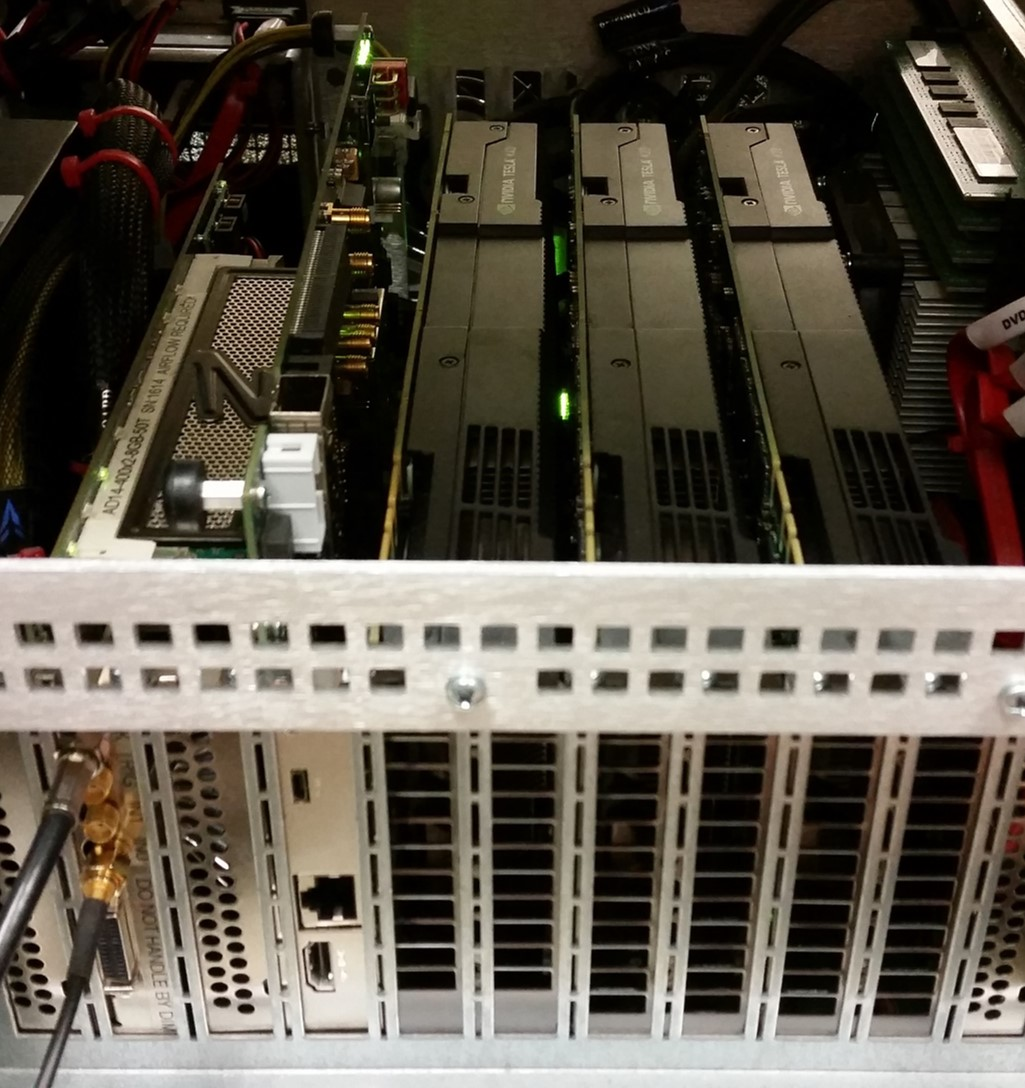
\includegraphics[scale=0.55]{figures/systemOverview/HostSystem.jpg}
	\caption{A picture of the physical PAQ project hardware refrencing blocks from Figure \ref{fig:hardwareblock}. Right: Components in the dashed and dotted box. Left: Components in the dashed box. Note that the T/M Receiver is not pictured.}
	\label{fig:HostSystem}
\end{figure}
The major components, and their functions are summarized in the following.
\begin{itemize}
	\item The \textbf{T/M mixer} down-converts from L or C band RF to IF (70 MHz) then applies an anti-aliasing filter.
	%
	\item The \textbf{rack mounted server} is a high powered computer that houses an ADC, a FPGA and three GPUs 		slotted into a 32 pin PCIe bus.
	\item The \textbf{ADC} produces 14-bit samples of the real-valued bandpass signal
	centered at IF sampled at $93\nicefrac{1}{3}$ Msamples/s.
	The samples are transferred to the host CPU via the PCIe bus.
	%
	\item The \textbf{host CPU} initiates memory transfers between itself and the ADC, GPUs and FPGA via the PCIe 	bus. 
	The host CPU also launches the digital signal processing algorithms on the GPUs.
	%
	\item The three \textbf{GPUs} are where all the detection, estimation, equalization and demodulation resides.
While the CPU has one to eight powerful processors, GPUs have thousands of small less powerful processors that work in parallel. The signal processing is done in GPUs rather than FPGAs or a CPU because programming GPUs is faster and easier than programming FPGAs and CPUs do not prosess the required processing power.
	%
	\item The \textbf{FPGA} receives all the bit streams from the host CPU via the PCIe bus then clocks each 			stream out in parallel to the BERT for BER testing.
	%
	\item The bit error rate tester (\textbf{BERT}) counts the errors in each input bit stream by comparing the 		streams to a PN sequence.
	%
	\item The \textbf{T/M Receiver} outputs bit streams for blind equalization and no equalization for 					BER comparison.
\end{itemize}
%A picture of the rack mounted physical system is shown in Figure \ref{fig:rack}.
%\begin{figure}
%	\centering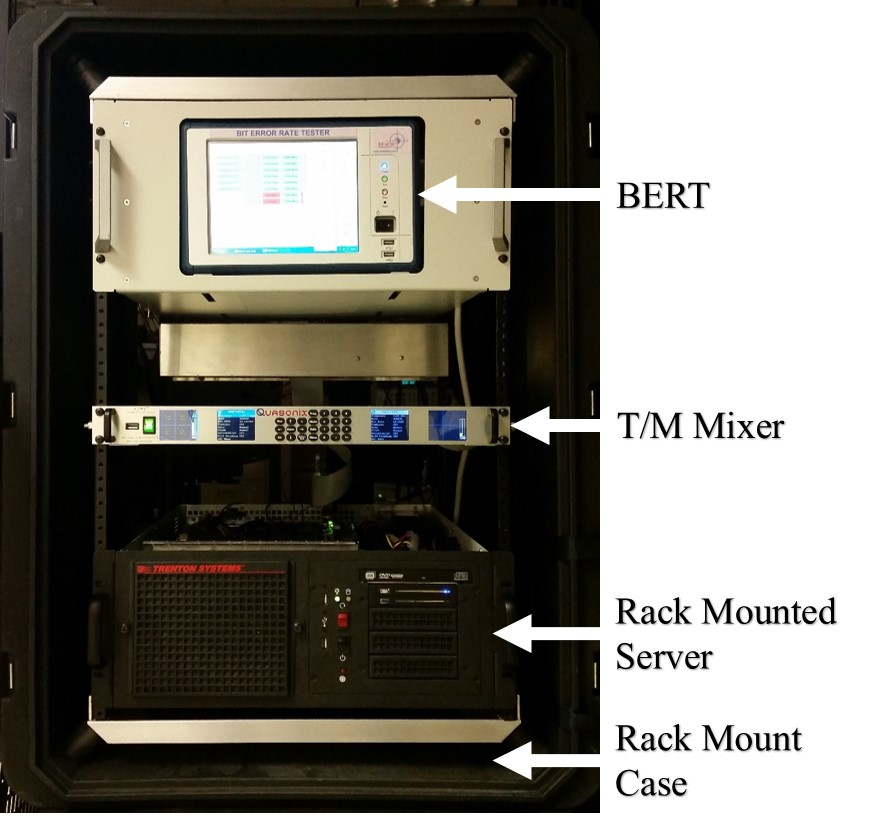
\includegraphics[scale=0.55]{figures/systemOverview/rack.jpg}
%	\caption{A picture of the physical PAQ project hardware. Note that the T/M Receiver is not pictured.}
%	\label{fig:rack}
%\end{figure}
%A picture of the components inside the rack mounted server is shown in Figure \ref{fig:rack}.
%\begin{figure}
%	\centering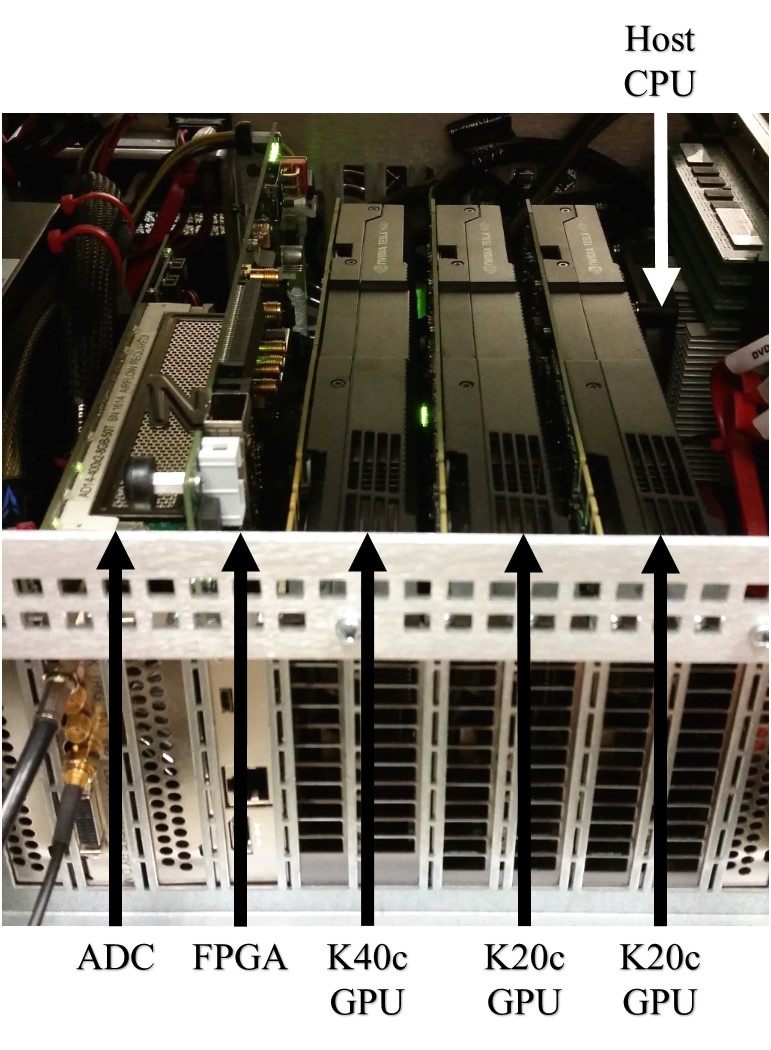
\includegraphics[scale=0.55]{figures/systemOverview/server.jpg}
%	\caption{A pictureof the components inside the rack mounted server.}
%	\label{fig:server}
%\end{figure}

To enable data-aided equalization, the PAQ project bit stream has a packetized structure shown in Figure \ref{fig:packetStructure_intro}.
The bit stream has a pilot bit sequence, in the form of the iNET preamble and ASM, periodically inserted into the data bits.
\begin{figure}
	\centering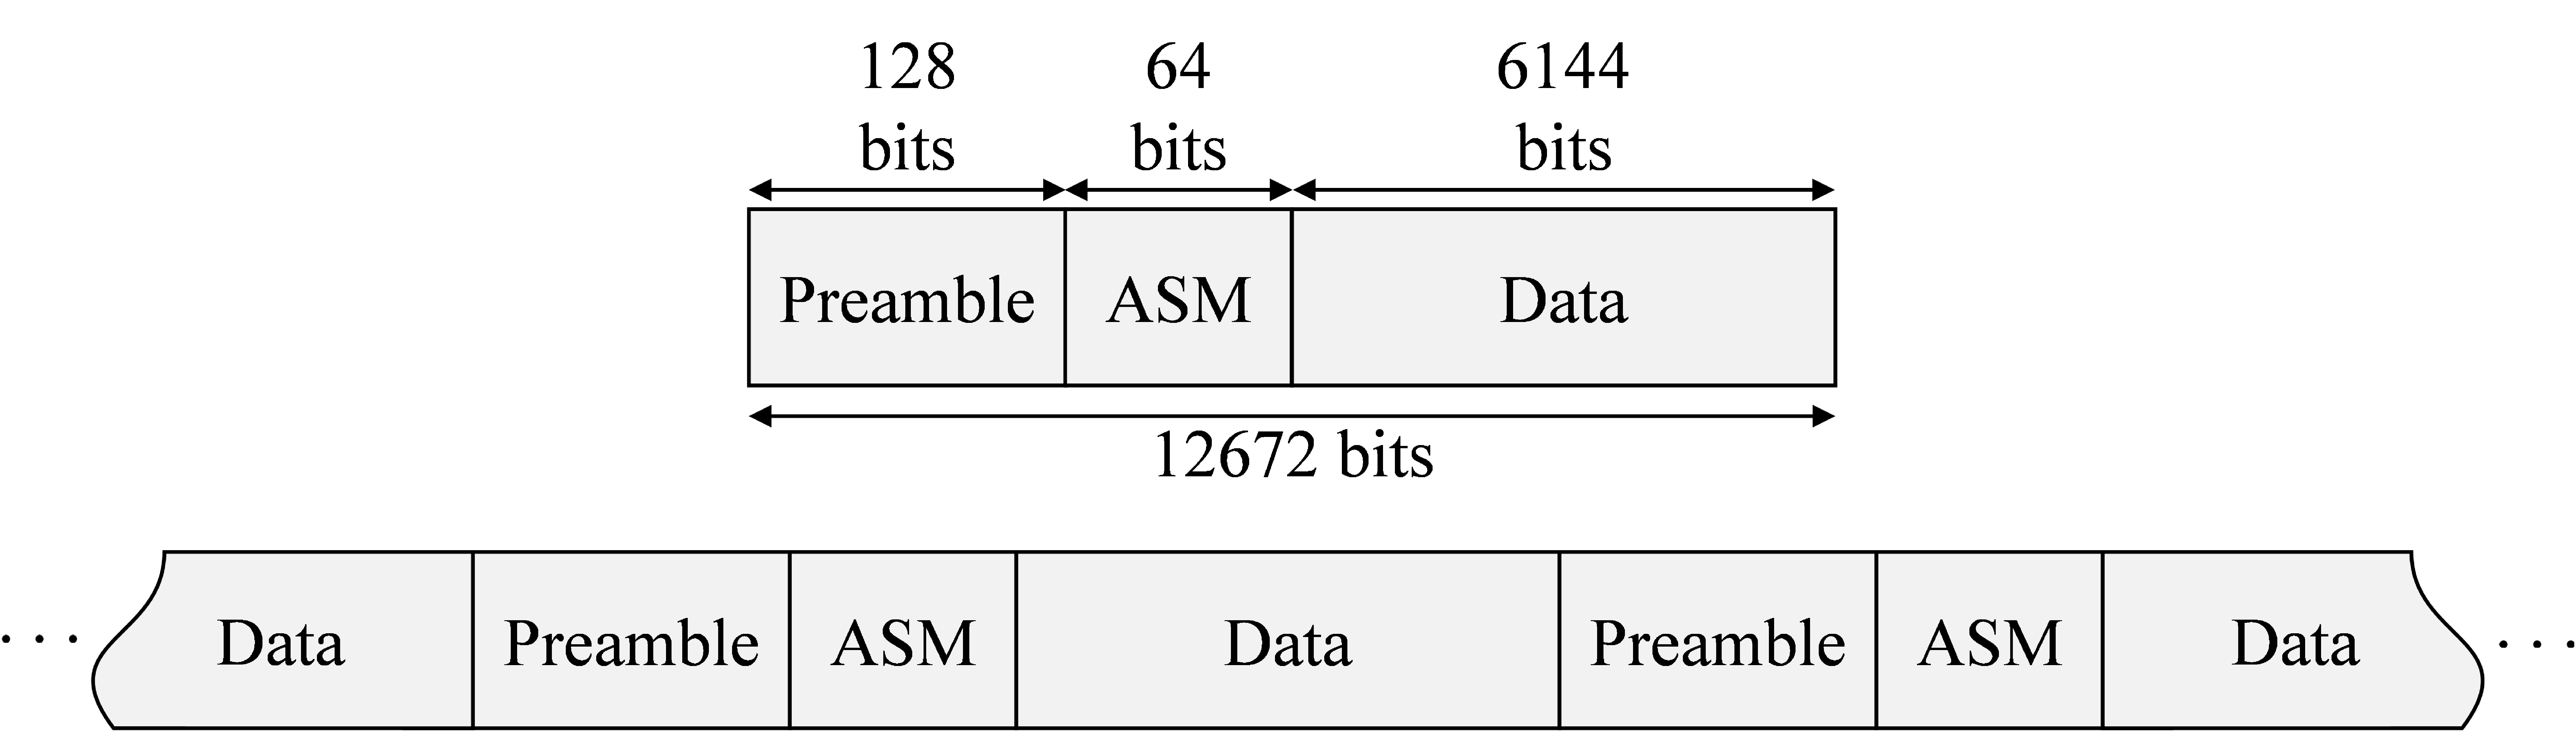
\includegraphics[width=9.47in/100*55]{figures/intro/packetSturcture.pdf}
	\caption{A diagram showing the PAQ packetized sample structure.}
	\label{fig:packetStructure_intro}
\end{figure}
The iNET preamble comprises eight repetitions of the 16-bit sequence $\text{CD98}_\text{hex}$ and the ASM field is
\begin{equation}
\text{034776C7272895B0}_\text{hex}.
\end{equation}
The data payload is a known length-$(2^{11} - 1)$ PN sequence.
Each packet contains $128$ preamble bits, $64$ ASM bits and $6{,}144$ data bits making each iNET packet $6{,}336$ bits.
The data bits modulate a SOQPSK-TG carrier at $10$ Mbits/second.
With the preamble and ASM periodically inserted, the over the air bit rate is $10.3125$ Mbits/second.

After modulation, the transmitted signal experiences multipath interference modeled as the channel $h(t)$.
The transmitted signal also experiences a frequency offset $\omega_0$, a phase offset $\phi$ and additive white Gaussian noise $w(t)$.
The received signal is down-converted, filtered in the T/M mixer, sampled at $93\nicefrac{1}{3}$ Msamples/second by the ADC then down-converted again to baseband and resampled by $\nicefrac{99}{448}$ in the GPUs resulting in the sampled sequence $r(n)$ at rate $20.625$ Msamples/second or $2$ samples/bit.

The model of the received signal is shown in Figure \ref{fig:received1}.
At baseband and $2$ samples/bit, the FIR channel impulse response is assumed to have a non-causal component comprising $N_1$ samples and a causal component comprising $N_2$ samples.
Figure \ref{fig:channelExample} shows the full discrete-time $L_h = N_1+N_2+1$ sample channel.
The received signal is sampled at $20.625$ Msamples/second.
The iNET packet is $\Lpkt=12672$ samples long with the preamble $L_\text{p}=256$ samples and the ASM $L_\text{ASM}=128$ samples.
\begin{figure}
	\centering
\includegraphics[width=12.33in/100*50]{figures/intro/received1.pdf}
	\caption{Received signal has multipath interference, frequency offset, phase offset and additive white Gaussian noise. The received signal is down-converted filtered and sampled to produce the sample sequence $r(n)$.}
	\label{fig:received1}
\end{figure}
\begin{figure}
	\centering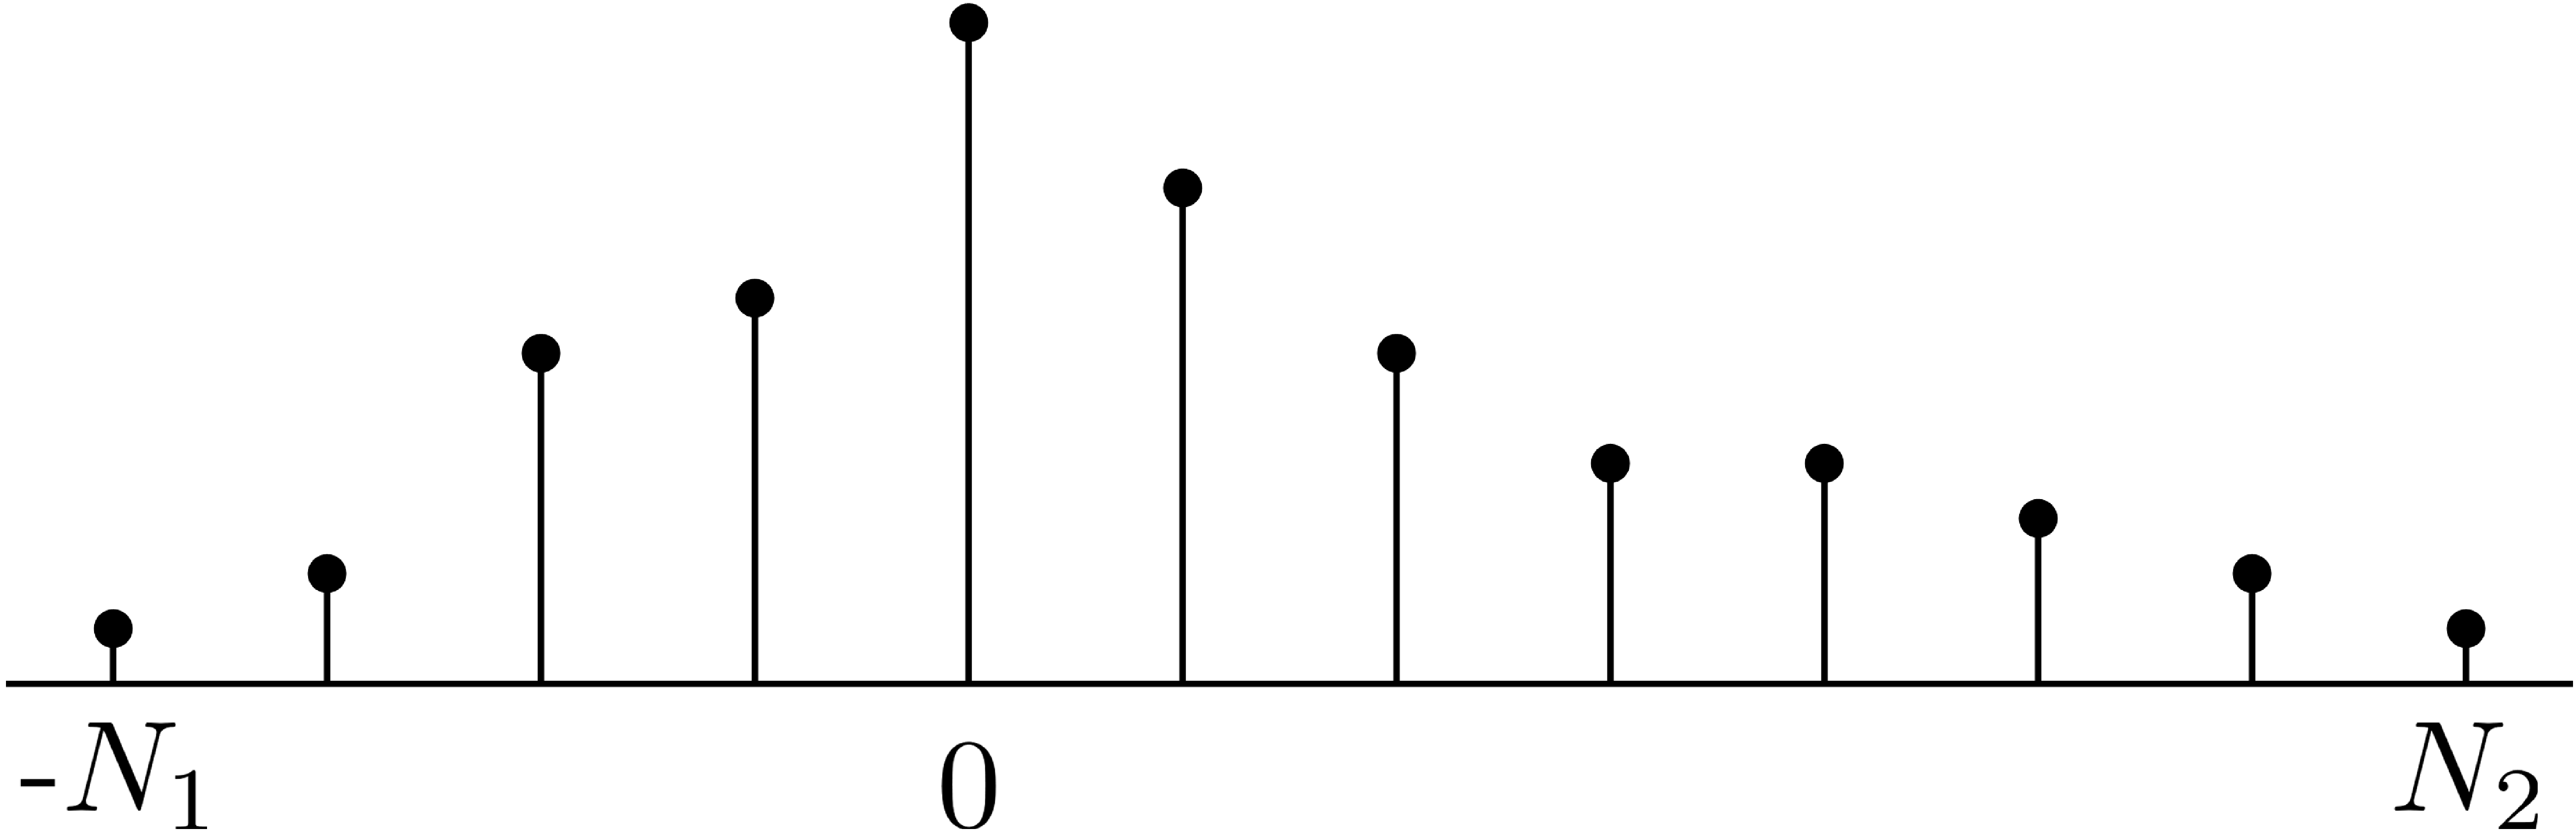
\includegraphics[width=5.5in/100*55]{figures/intro/channelExample.pdf}
	\caption{An illustration of the discrete-time channel of length $N_1+N_2+1$ with a non-causal component comprising $N_1$ samples and a causal component comprising $N_2$ samples.}
	\label{fig:channelExample}
\end{figure}

\section{Digital Signal Processing}
\label{sec:signalProcessing}
A high-level digital signal processing flow is shown in Figure \ref{fig:estimators} and \ref{fig:thisThesisBlock}.
Because the frequency offset, channel, and noise variance are estimated using the preamble and ASM, the first step is to find the samples correlating to the preamble in the received sample sequence $r(n)$.
The preamble detector block correlates received samples with $L_\text{P}$ samples of a locally stored copy of the pilot in \eqref{eq:preamble_ASM}.
The preamble detector block outputs the vector of samples $\mathbf{r}_\text{p}$ with the iNET packetized structure.
The first $L_\text{P} + L_\text{ASM}$ samples in $\mathbf{r}_\text{p}$ correlate with the received pilot samples.
\begin{equation}
\mathbf{p} = \big[ p(0) \quad p(1) \quad \cdots  \quad  p(L_\text{P} + L_\text{ASM}-1) \big]
\label{eq:preamble_ASM}
\end{equation}

The located preamble samples are used first to estimate the frequency offset.
The estimated frequency offset $\hat{\omega}_0$ rads/sample is then used to ``de-rotate'' the vector of samples $\mathbf{r}_\text{p}$ to produce $\mathbf{r}$.
The de-rotated samples in the vector $\mathbf{r}$ that correlate to the preamble and ASM are used to estimate the channel $\hat{\mathbf{h}}$ and noise variance $\hat{\sigma}^2_w$.
The channel and noise variance estimates are done in the estimators block.
\begin{figure}
	\centering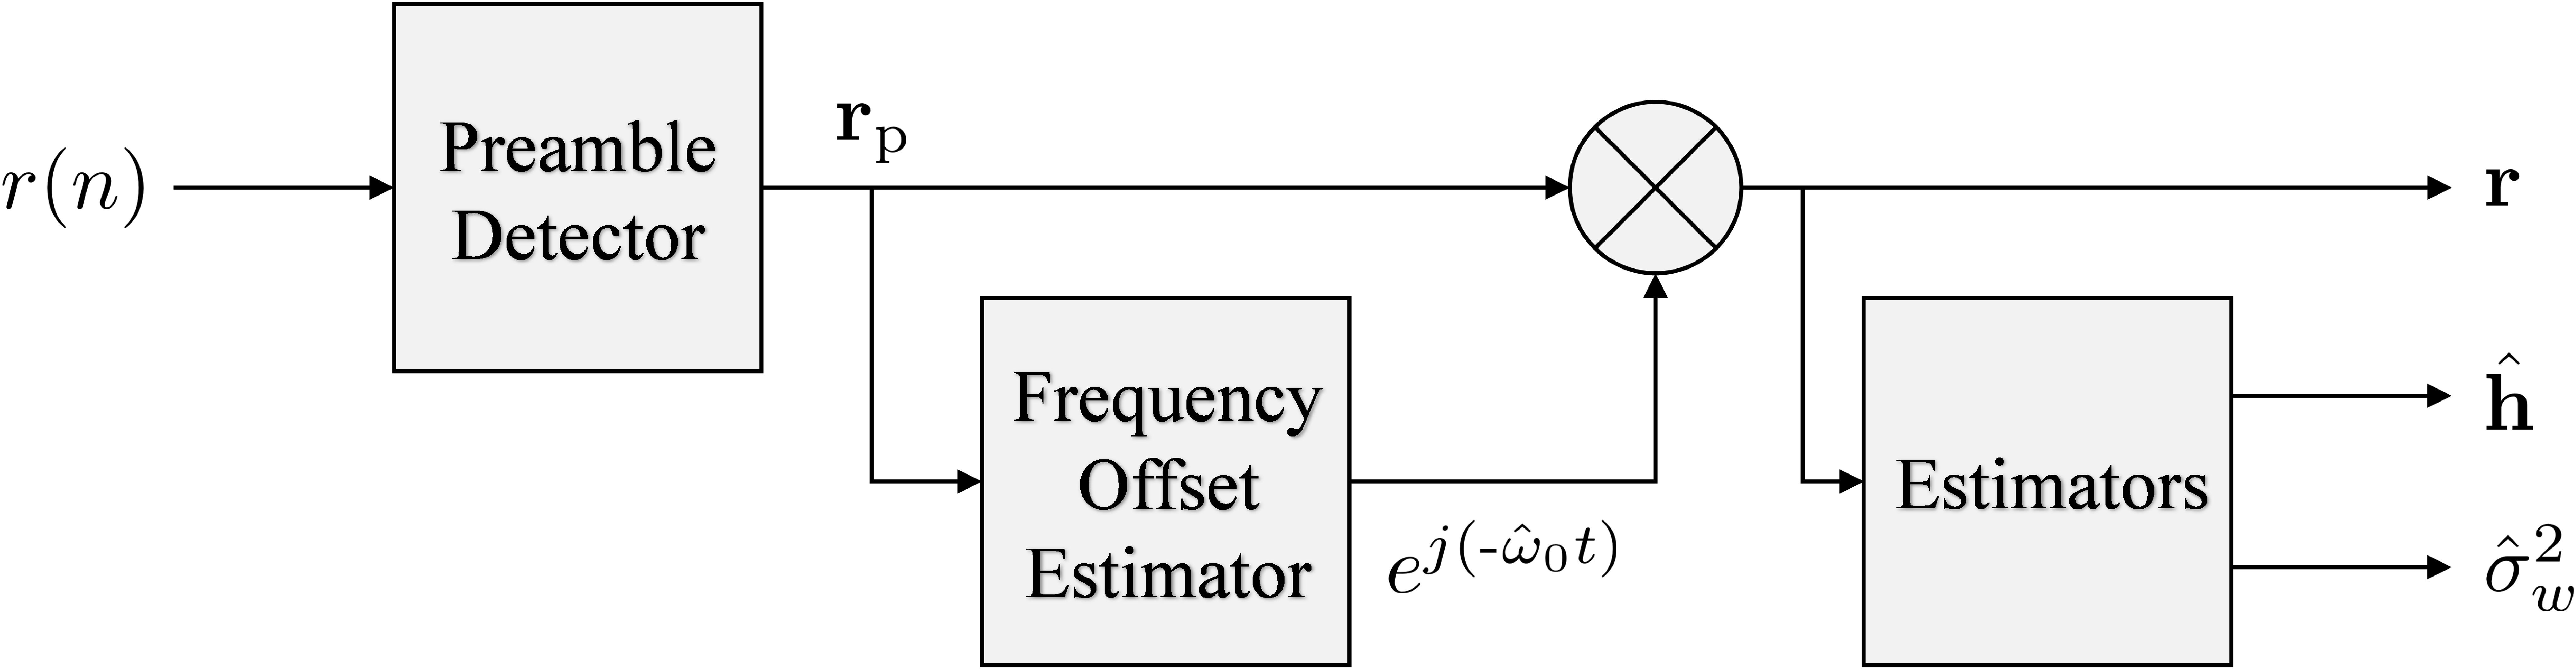
\includegraphics[width=8.75in/100*55]{figures/intro/estimators.pdf}
	\caption{A block diagram of the estimators in the PAQ project.}
	\label{fig:estimators}
\end{figure}

Equipped with knowledge of the estimated channel and noise variance, data-aided finite impulse response (FIR) equalizer filters can be computed.
The all the data-aided equalizer filters are computed using the same channel and noise variance estimates.
The blocks shown in Figure \ref{fig:thisThesisBlock} are duplicated in five independent branches producing five estimated vectors of bits $\hat{\mathbf{b}}$, one for each equalizer.

%An equalizer filter is computed using the channel estimate $\hat{\mathbf{h}}$ and noise variance $\hat{\sigma}^2_w$ then applied to the vector of samples $\mathbf{r}$.
The PAQ project designed the data-aided FIR equalizer filters to be $5$ times longer than the channel estimate. The equalizer filter has a non-causal component comprising $L_1 = 5N_1 = 60$ samples and a causal component comprising $L_2 = 5N_2 = 125$ samples.
The $L_\text{EQ} = L_1+L_2+1$ sample full discrete-time equalizer filters are computed and applied in the equalizer filter block.

The output of the equalizer filters are then filtered by a SOQPSK-TG detection filter and down-sampled by $2$ in preparation for an OQPSK detector.
The $\mathbf{r}_\text{d}$ in each equalizer branch has a sample rate of $1$ sample/bit or $2$ samples/symbol.
The OQPSK detector block outputs the vector of estimated bits $\hat{\mathbf{b}}$.
\begin{figure}
	\centering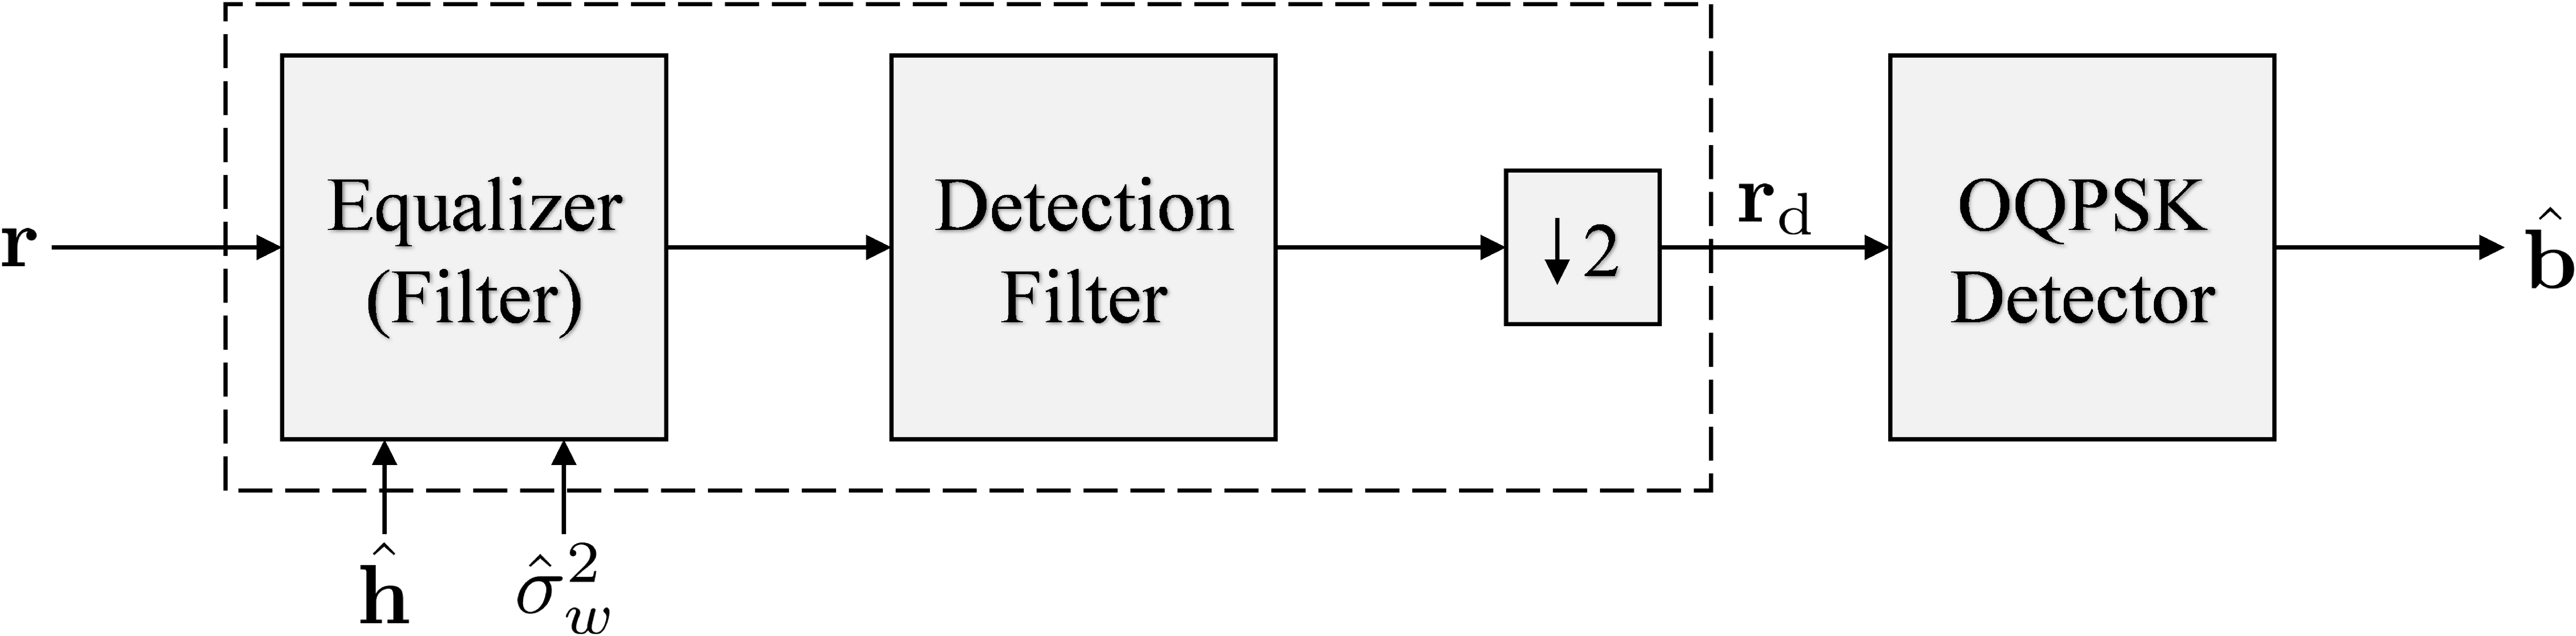
\includegraphics[width=8.37in/100*55]{figures/intro/thisThesisBlock.pdf}
	\caption{A block diagram of application of the FIR equalizer and detection filters in the Preamble Assisted Equalization (PAQ) project.}
	\label{fig:thisThesisBlock}
\end{figure}
Finally the BER for each equalizer is obtained by comparing the vectors of estimated bits $\hat{\mathbf{b}}$ to the PN sequence.

The GPUs in Figure \ref{fig:hardwareblock} and \ref{fig:HostSystem} perform all the digital signal processing in parallel.
To introduce as much parallelism as possible, the received samples are processed in $39$,$321$,$600$ sample 		sets. 
At $20.625$ Msamples/second, each set of $39$,$321$,$600$ samples is $1907$ milliseconds worth of data.
Each set has at most $3104$ independent $12672$ sample iNET packets.
The GPU processes $3104$ packets in parallel by leveraging batched processing.
Each packet is a batch and each batch performs the algorithms shown in Figures \ref{fig:estimators} and \ref{fig:thisThesisBlock}.
In order to stay real-time, \textbf{all} processing must be completed in $1907$ ms.

This thesis, will illustrate how the five PAQ data-aided equalizers were computed and applied to the received samples in GPUs.
The dashed box in Figure \ref{fig:thisThesisBlock} emphasizes which processing blocks are focused on.

Chapter \ref{chap:equations} shows the equations for these block diagrams.
Chapter \ref{chap:gpu} will shed some light on signal processing in GPUs.
Chapter \ref{chap:equalizers_in_gpus} will illustrate how the five equalizers are implemented in GPUs.
Chapter \ref{chap:final_summary} will summarize.
\include{Estimators}
%%%%%%%%%%%%%%%%%%%%%%%%%%%%%%%%%%%%%%%%%%%%%%%%%%%%%%%%%%%%%%%%%%%%%%%%%%%%%%%%%%%%%%%%%%%%%%
%%%%%%%%%%%%%%%%%%%%%%%%%%%%%%%%%%%%%%%%%%%%%%%%%%%%%%%%%%%%%%%%%%%%%%%%%%%%%%%%%%%%%%%%%%%%%%
%%%%%%%%%%% GPU
%%%%%%%%%%%%%%%%%%%%%%%%%%%%%%%%%%%%%%%%%%%%%%%%%%%%%%%%%%%%%%%%%%%%%%%%%%%%%%%%%%%%%%%%%%%%%%
%%%%%%%%%%%%%%%%%%%%%%%%%%%%%%%%%%%%%%%%%%%%%%%%%%%%%%%%%%%%%%%%%%%%%%%%%%%%%%%%%%%%%%%%%%%%%%


% \cleardoublepage
\chapter{Signal Processing with GPUs}
\label{sec:gpu}

This thesis explores the use of GPUs in data-aided estimation, equalization and filtering operations.

A Graphics Processing Unit (GPU) is a computational unit with a highly-parallel architecture well-suited for executing the same function on many data elements.
In the past, GPUs were used to process graphics data.
Recently, general purpose GPUs are being used for high performance computing in computer vision, deep learning, artificial intelligence and signal processing \cite{wikipedia-gpu:2015}.

GPUs cannot be programmed the way as a CPU. 
NVIDIA released a extension to C, C++ and Fortran called CUDA (Compute Unified Device Architecture).
CUDA allows a programmer to write C++ like functions that are massively parallel called \textit{kernels}.
To invoke parallelism, a GPU kernel is called $N$ times and mapped to $N$ \textit{threads} that run concurrently.
To achieve the full potential of high performance GPUs, kernels must be written with some basic concepts about GPU architecture and memory in mind.

The purpose of this overview is to provide context for the contributions of this thesis.
As such this overview is not a tutorial.
For a full explination of CUDA programming please see the CUDA toolkit documentation \cite{CUDA_toolkit_doc}.

\section{Simple GPU code example}
If a programmer has some C++ experience, learning how to program GPUs using CUDA comes fairly easily.
GPU code still runs top to bottom and memory still has to be allocated.
The only real difference is where the memory physically is and how functions run on GPUs.
To run functions or kernels on GPUs, the memory must be copied from the host (CPU) to the device (GPU).
Once the memory has been copied, the parallel GPU kernels can be called.
After the GPU kernels have finished, the resulting memory has to be copied back from the device (GPU) to the host (CPU).

Listing \ref{code:GPUvsCPU} shows a simple program that sums to vectors together
\begin{equation}
\begin{matrix}
\mathbf{C}_1 = \mathbf{A}_1 + \mathbf{B}_1 \\
\mathbf{C}_2 = \mathbf{A}_2 + \mathbf{B}_2
\end{matrix}
\end{equation}
where each vector is length $1024$.
Figure \ref{fig:CPUaddBlockDiagram} shows how the CPU computes $\mathbf{C}_1$ by summing elements of $\mathbf{A}_1$ and $\mathbf{B}_1$ together \textit{sequentially}.
Figure \ref{fig:GPUaddBlockDiagram} shows how the GPU computes $\mathbf{C}_2$ by summing elements of $\mathbf{A}_1$ and $\mathbf{B}_1$ together \textit{in parallel}.
The GPU kernel computes every element of $\mathbf{C}_2$ in parallel while the CPU computes one element of $\mathbf{C}_1$ at a time.
\begin{figure}
	\centering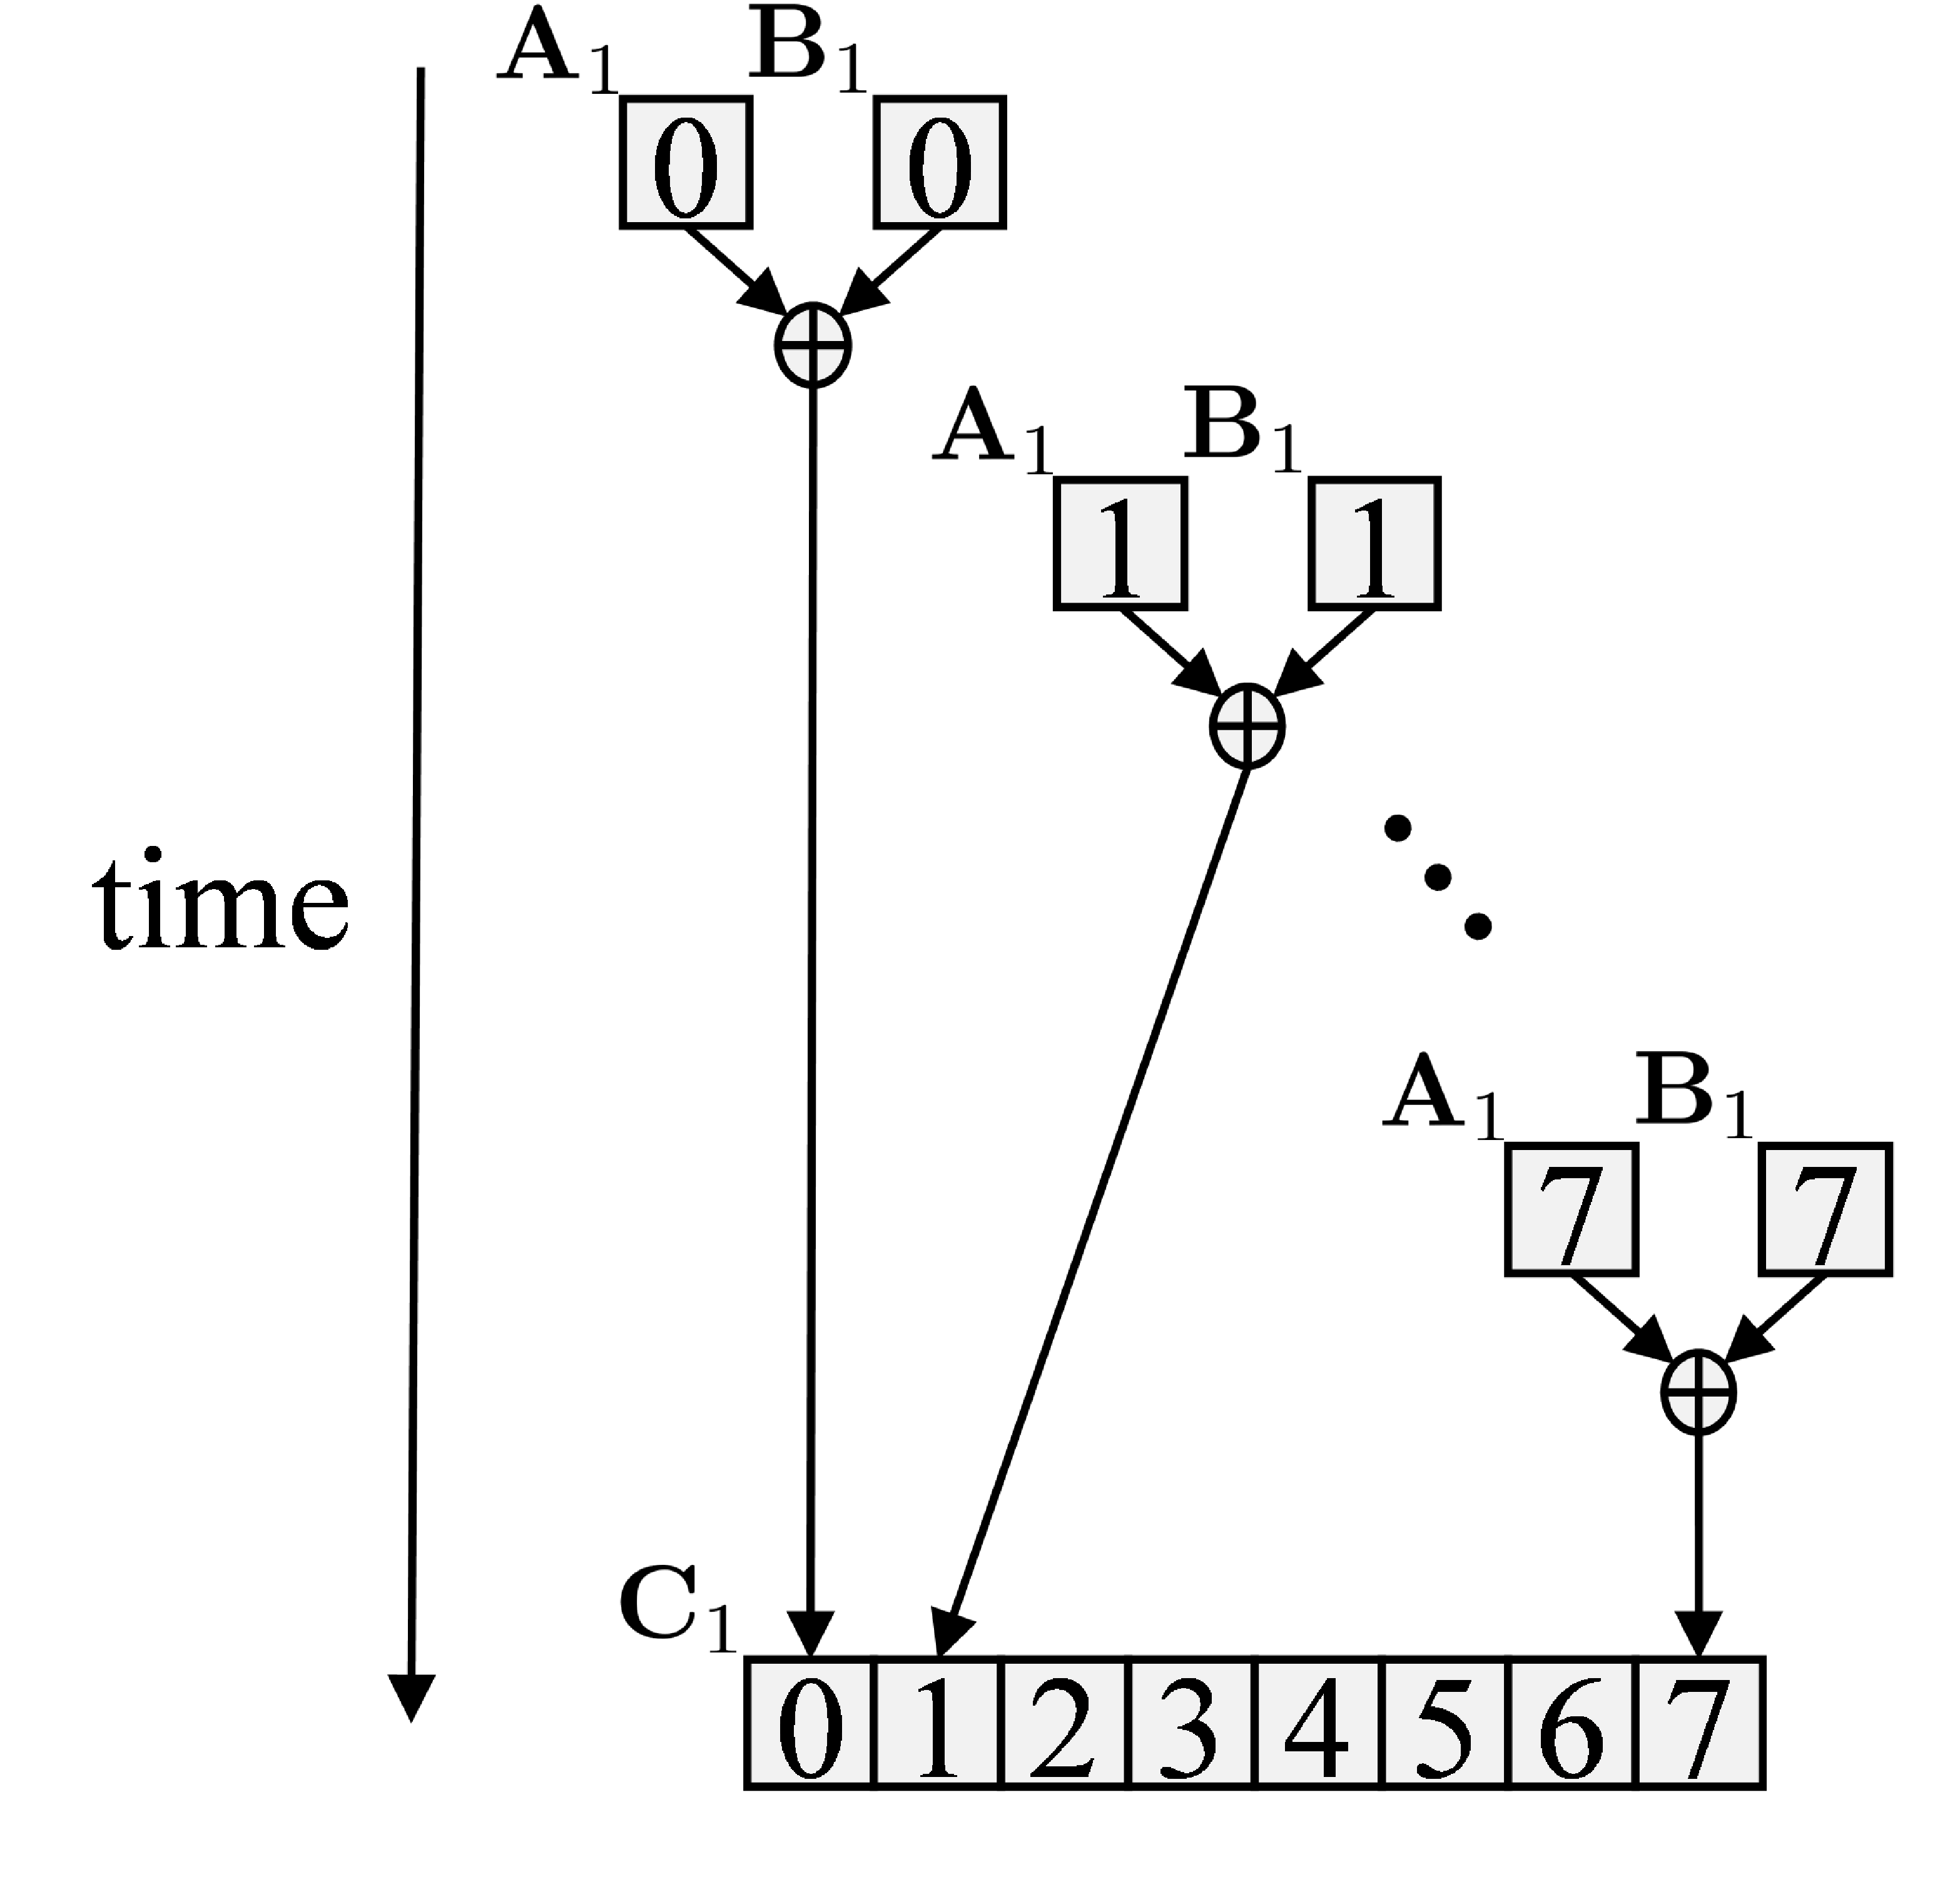
\includegraphics[width=3.17in/100*55]{figures/gpu_intro/CPUaddBlockDiagram.pdf}
	\caption{A block diagram of how a CPU sequentially performs vector addition.}
	\label{fig:CPUaddBlockDiagram}
\end{figure}
\begin{figure}
	\centering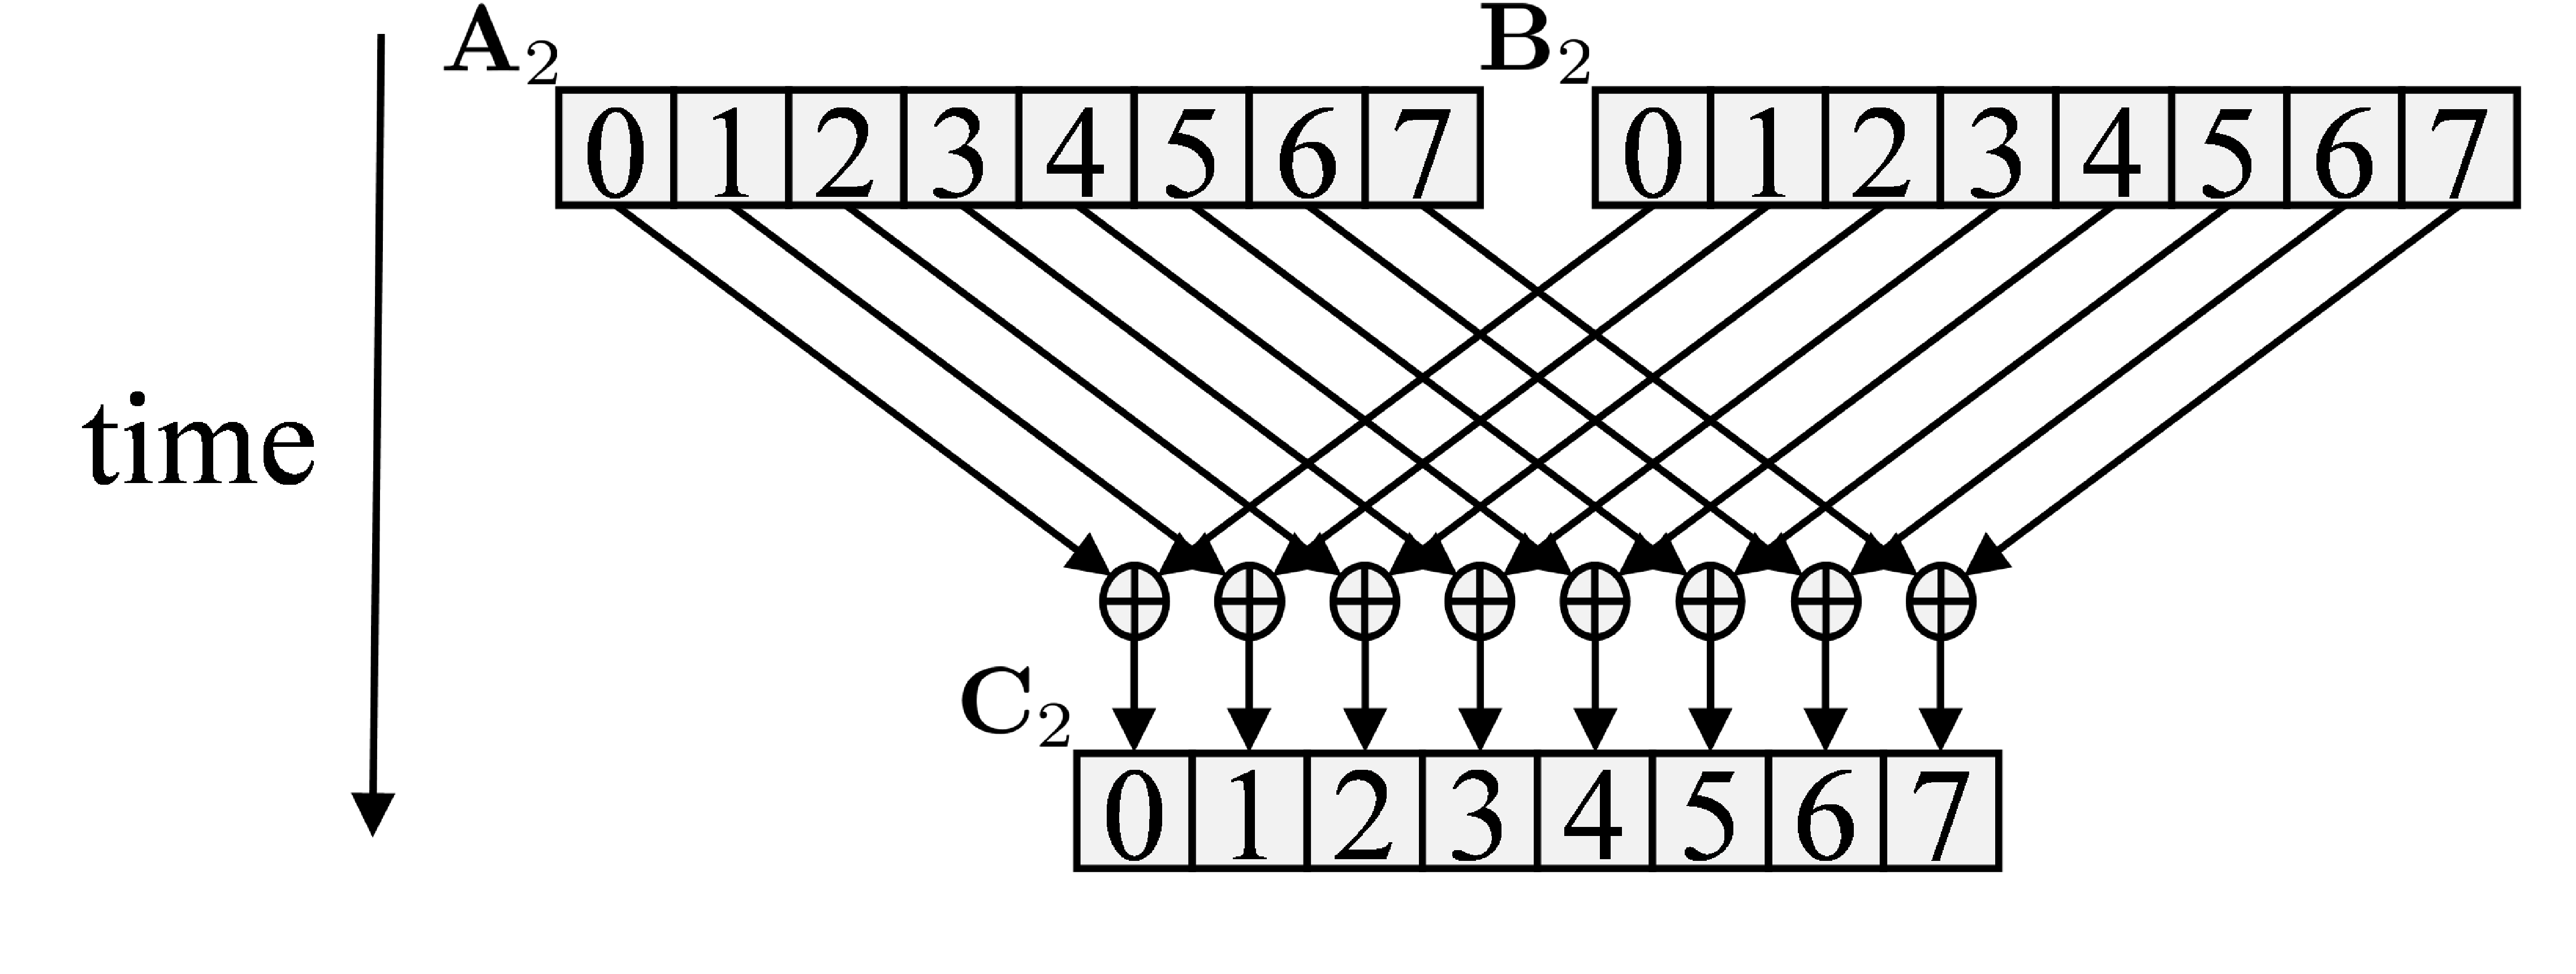
\includegraphics[width=4.69in/100*55]{figures/gpu_intro/GPUaddBlockDiagram.pdf}
	\caption{A block diagram of how a GPU performs vector addition in parallel.}
	\label{fig:GPUaddBlockDiagram}
\end{figure}
\singlespacing
\clearpage
\begin{lstlisting}[caption={Comparison of CPU verse GPU code.},label={code:GPUvsCPU}]
#include <iostream>
#include <stdlib.h>
#include <math.h>
using namespace std;

void VecAddCPU(int* destination,int* source0,int* source1,int myLength){
	for(int i = 0; i < myLength; i++)
		destination[i] = source0[i] + source1[i];
}

__global__ void VecAddGPU(int* destination, int* source0, int* source1, int lastThread){
	int i = blockIdx.x*blockDim.x + threadIdx.x;

	// don't access elements out of bounds
	if(i >= lastThread)
		return;

	destination[i] = source0[i] + source1[i];
}

int main(){
	int numPoints = pow(2,22);
	cout << numPoints << endl;
	/*--------------------------------------------------------------------
                               	   CPU Start
	--------------------------------------------------------------------*/
	// allocate memory on host
	int *A1;
	int *B1;
	int *C1;
	A1 = (int*) malloc (numPoints*sizeof(int));
	B1 = (int*) malloc (numPoints*sizeof(int));
	C1 = (int*) malloc (numPoints*sizeof(int));

	// Initialize vectors 0-99
	for(int i = 0; i < numPoints; i++){
		A1[i] = rand()%100;
		B1[i] = rand()%100;
	}

	// vector sum C1 = A1 + B1
	VecAddCPU(C1, A1, B1, numPoints);
	/*--------------------------------------------------------------------
                               	   CPU End
	--------------------------------------------------------------------*/

	/*--------------------------------------------------------------------
                               	   GPU End
	--------------------------------------------------------------------*/
	// allocate memory on host for result
	int *C2;
	C2 = (int*) malloc (numPoints*sizeof(int));

	// allocate memory on device for computation
	int *A2_gpu;
	int *B2_gpu;
	int *C2_gpu;
	cudaMalloc(&A2_gpu, sizeof(int)*numPoints);
	cudaMalloc(&B2_gpu, sizeof(int)*numPoints);
	cudaMalloc(&C2_gpu, sizeof(int)*numPoints);

	// Copy vectors A and B from host to device
	cudaMemcpy(A2_gpu, A1, sizeof(int)*numPoints, cudaMemcpyHostToDevice);
	cudaMemcpy(B2_gpu, B1, sizeof(int)*numPoints, cudaMemcpyHostToDevice);

	// Set optimal number of threads per block
	int numTreadsPerBlock = 32;

	// Compute number of blocks for set number of threads
	int numBlocks = numPoints/numTreadsPerBlock;

	// If there are left over points, run an extra block
	if(numPoints % numTreadsPerBlock > 0)
		numBlocks++;

	// Run computation on device
	//for(int i = 0; i < 100; i++)
		VecAddGPU<<<numBlocks, numTreadsPerBlock>>>(C2_gpu, A2_gpu, B2_gpu, numPoints);

	// Copy vector C2 from device to host
	cudaMemcpy(C2, C2_gpu, sizeof(int)*numPoints, cudaMemcpyDeviceToHost);
	/*--------------------------------------------------------------------
                               	   GPU End
	--------------------------------------------------------------------*/

	// Free vectors on CPU
	free(A1);
	free(B1);
	free(C1);
	free(C2);

	// Free vectors on GPU
	cudaFree(A2_gpu);
	cudaFree(B2_gpu);
	cudaFree(C2_gpu);
}
\end{lstlisting}
\doublespacing

\section{GPU kernel using threads and thread blocks}
A GPU kernel is executed on a GPU by launching numTreadsPerBlock$\times$numBlocks 
threads.
Each thread has a unique index.
CUDA calls this indes threadIdx and blockIdx.
threadIdx is the thread index inside the assigned thread block.
blockIdx is the index of the block the thread is assigned.
blockDim is the number of threads assigned per block, in fact blockDim $=$ numTreadsPerBlock.
Both threadIdx and blockIdx are three dimensional and have x, y and z components.
In this thesis only the x dimension is used because GPU kernels operate only on vectors.

To replace a CPU for loop that runs $0$ to $N-1$, a GPU kernel launches $N$ threads are with $T$ threads per thread block.
The number of blocks need is $M = \frac{N}{T}$ or $M = \frac{N}{T}+1$ if $N$ is not an integer multiple of $T$.
Figure \ref{fig:threadsBlocks32} shows $32$ threads launched in $4$ thread blocks with $8$ threads per block.
Figure \ref{fig:threadsBlocks36} shows $36$ threads launched in $5$ thread blocks with $8$ threads per block. An full extra thread block must be launched to with $8$ threads but $4$ threads are idle.
\begin{figure}
	\centering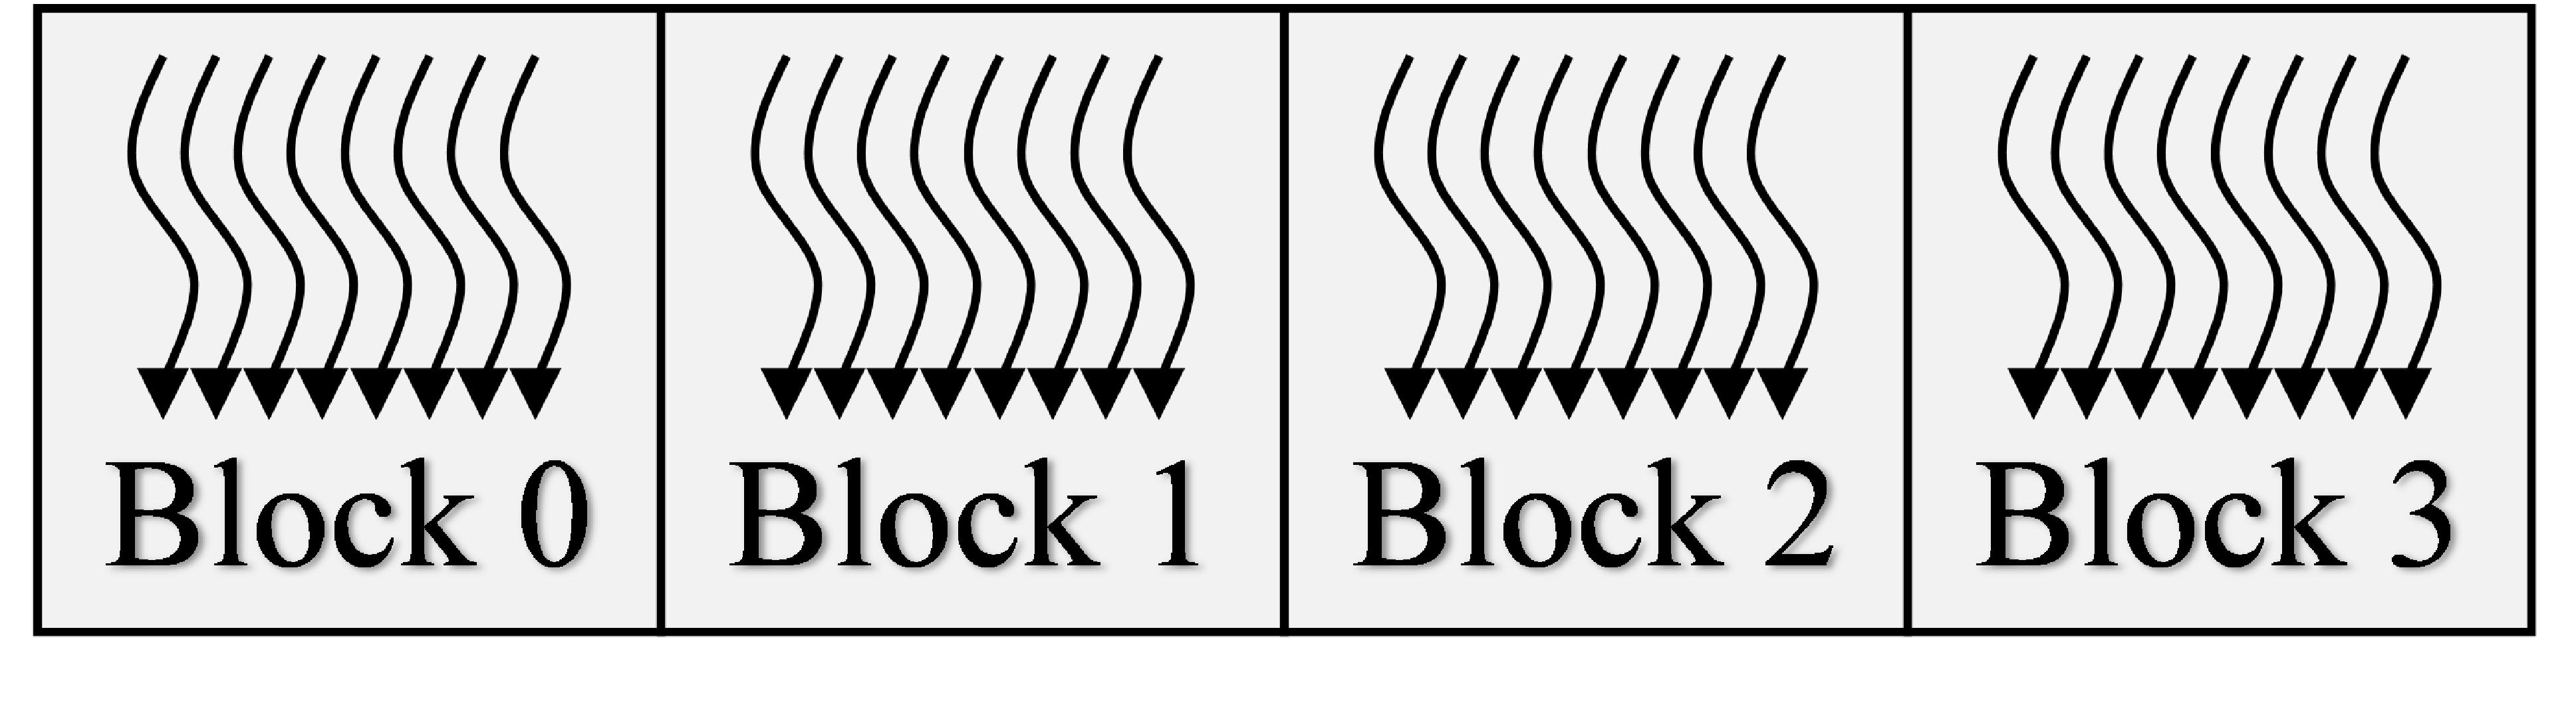
\includegraphics[width=4in/100*55]{figures/gpu_intro/threadsBlocks32.pdf}
	\caption{Block $0$ $32$ threads launched in $4$ thread blocks with $8$ threads per block.}
	\label{fig:threadsBlocks32}
\end{figure}
\begin{figure}
	\centering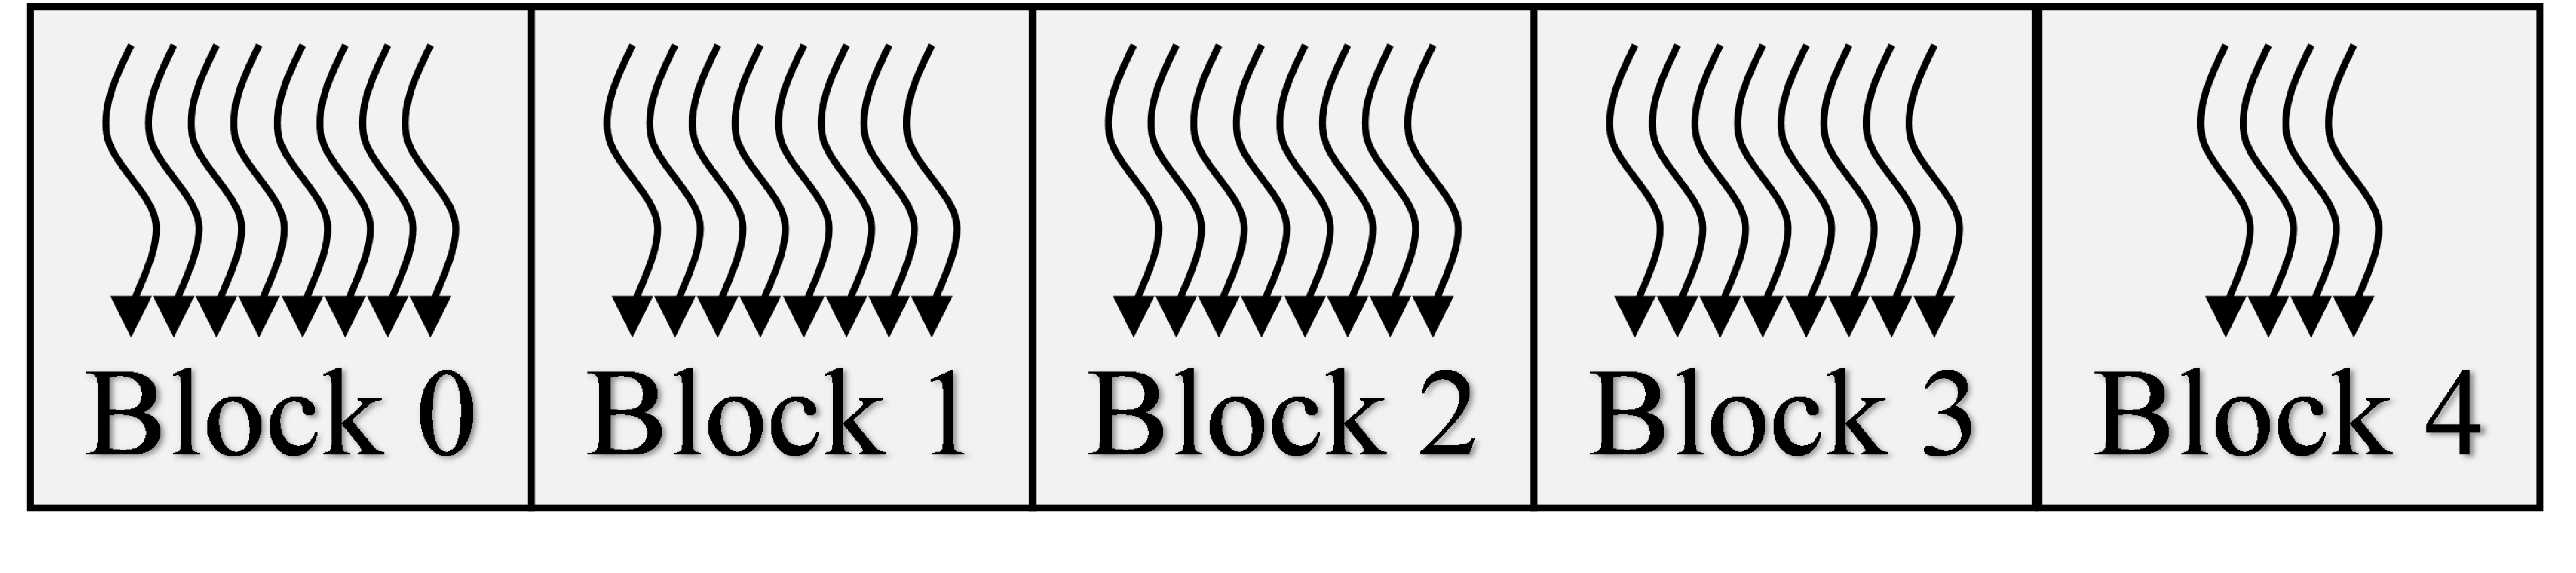
\includegraphics[width=5in/100*55]{figures/gpu_intro/threadsBlocks36.pdf}
	\caption{$36$ threads launched in $5$ thread blocks with $8$ threads per block with $4$ idle threads.}
	\label{fig:threadsBlocks36}
\end{figure}

\section{GPU memory}
Thread blocks run independent of other thread blocks.
The GPU does not guarantee Block $0$ will execute before Block $2$.
Threads in blocks can coordinate and use shared memory but blocks do not coordinate with other blocks.
Threads have access to private local memory that is fast and efficient.
Each thread in a thread block has access to private shared memory in the thread block.
All threads have access to global memory.

Local memory is the fastest and global memory is by far the slowest.
One global memory access takes 400-800 clock cycles while a local memory is a few clock cycles.
Why not just do all computations in local memory?
The memory needs come from global memory to before it can be used in local memory.
Memory should be saved in shared memory if many threads are going to use it in a thread block.
Local and shared memory should be used as much as possible but sometimes a GPU kernel cant utilized local and shared memory because elements might only be used once.
\begin{sidewaysfigure}
	\centering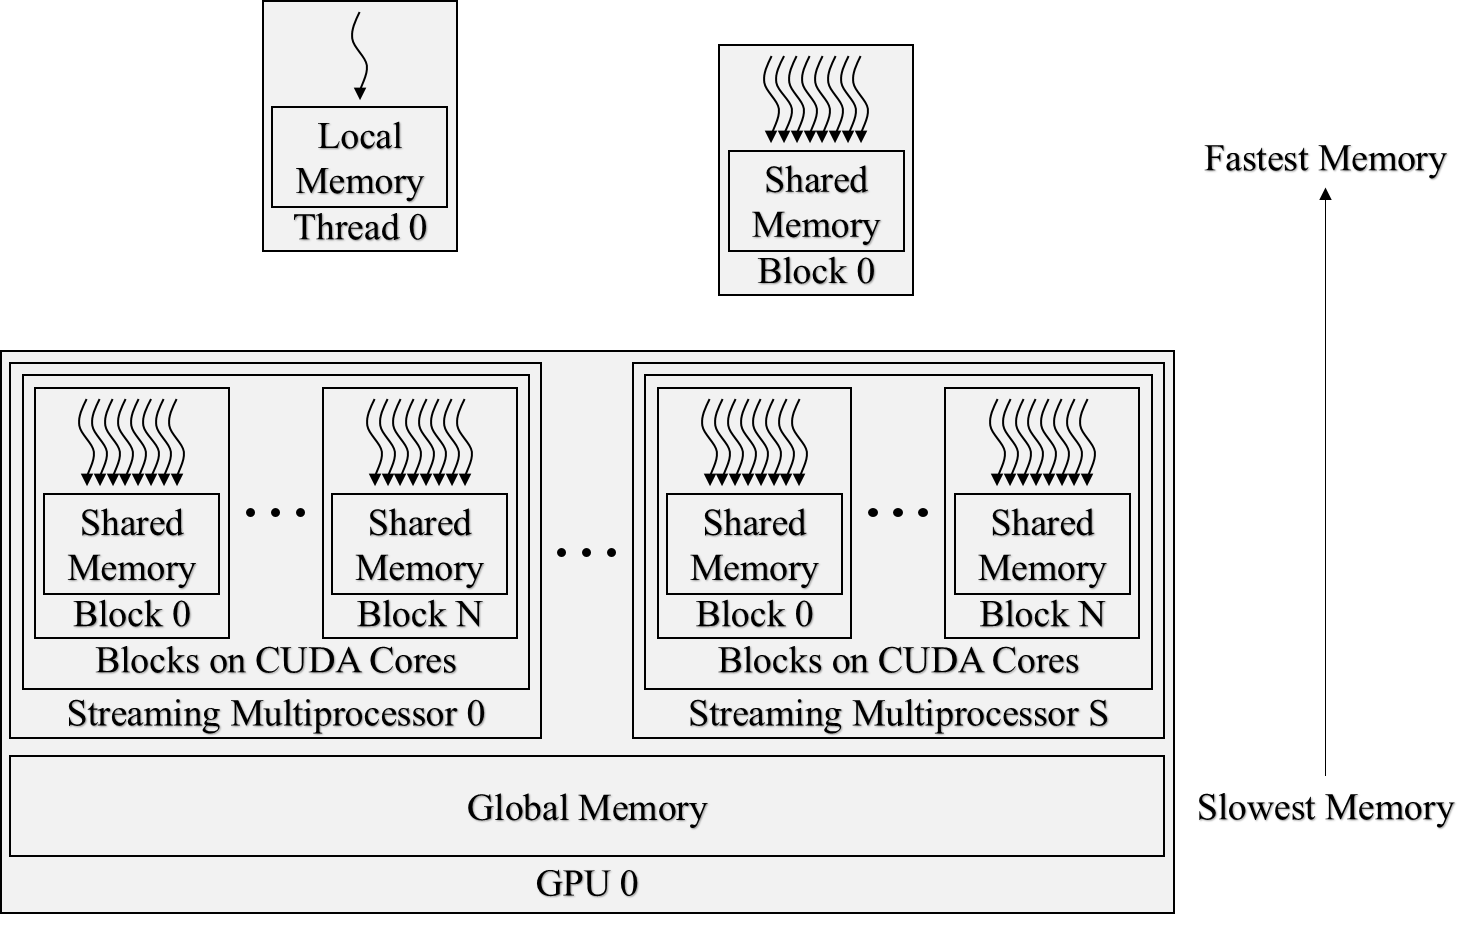
\includegraphics[width=9in/100*55]{figures/gpu_intro/fullGPUmemBlockDiagram.png}
	\caption{A block diagram where local, shared, and global memory is located. Each thread has private local memory. Each thread block has private shared memory. The GPU has global memory that all threads can access.}
	\label{fig:fullGPUmemBlockDiagram}
\end{sidewaysfigure}

Why is global memory so slow?
Looking at the physical hardware will shed some light.
This thesis uses NVIDIA Tesla K40c and K20c GPUs, Table \ref{tab:gpu-resources_jeffs} gives some specifications and Figure \ref{fig:GPUpicture} shows the form factor of the these GPUs.
The red box in Figure \ref{fig:GPUarch} show the GPU chip and the yellow boxes show the SRAM that is \textit{off} the GPU chip.
The GPU global memory is located in the SRAM.
To move memory to thread blocks \textit{on} the GPU chip from global memory requires fetching memory from \textit{off} the GPU.
Now 400-800 clock cycles doesn't sound all the bad huh?
\begin{figure}
	\centering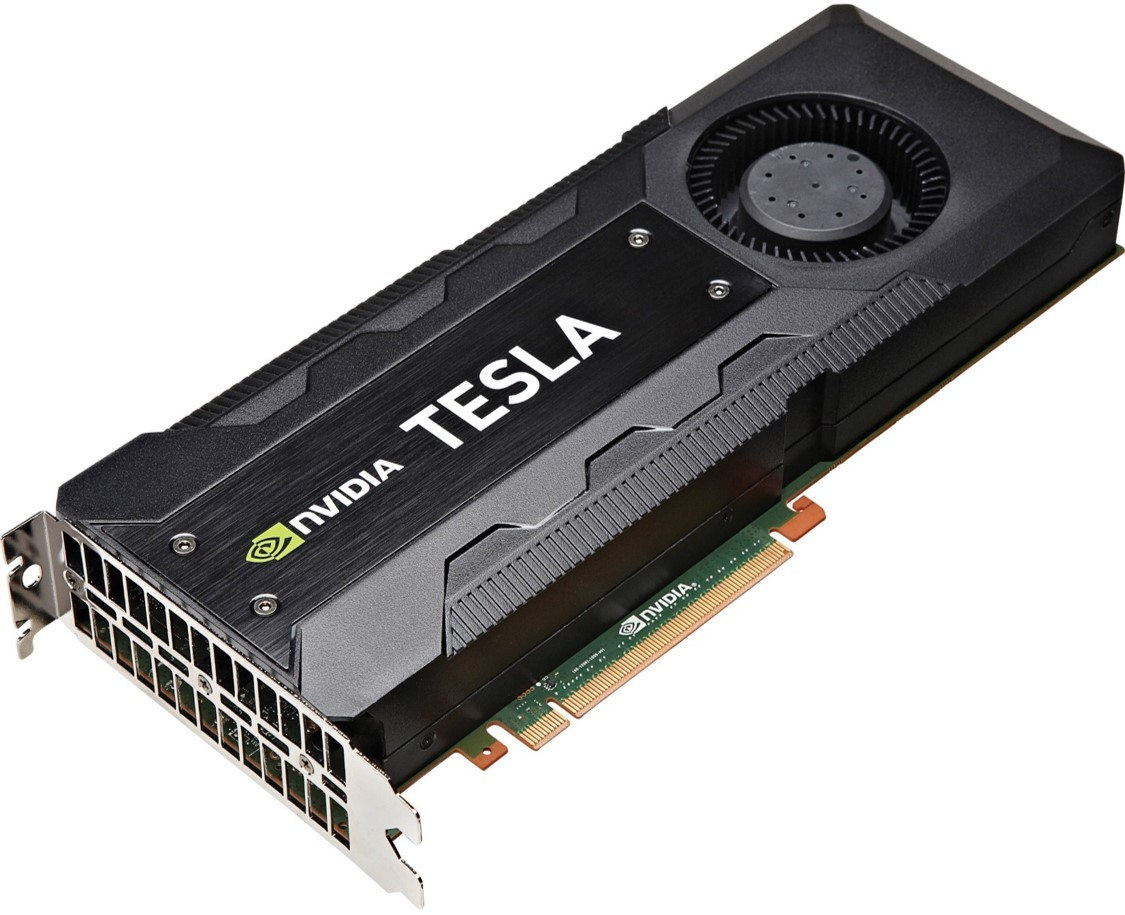
\includegraphics[width=5in]{figures/gpu_intro/k40c_k20c.jpg}
	\caption{NVIDIA Tesla K40c and K20c.}
	\label{fig:GPUpicture}
\end{figure}
\begin{figure}
	\centering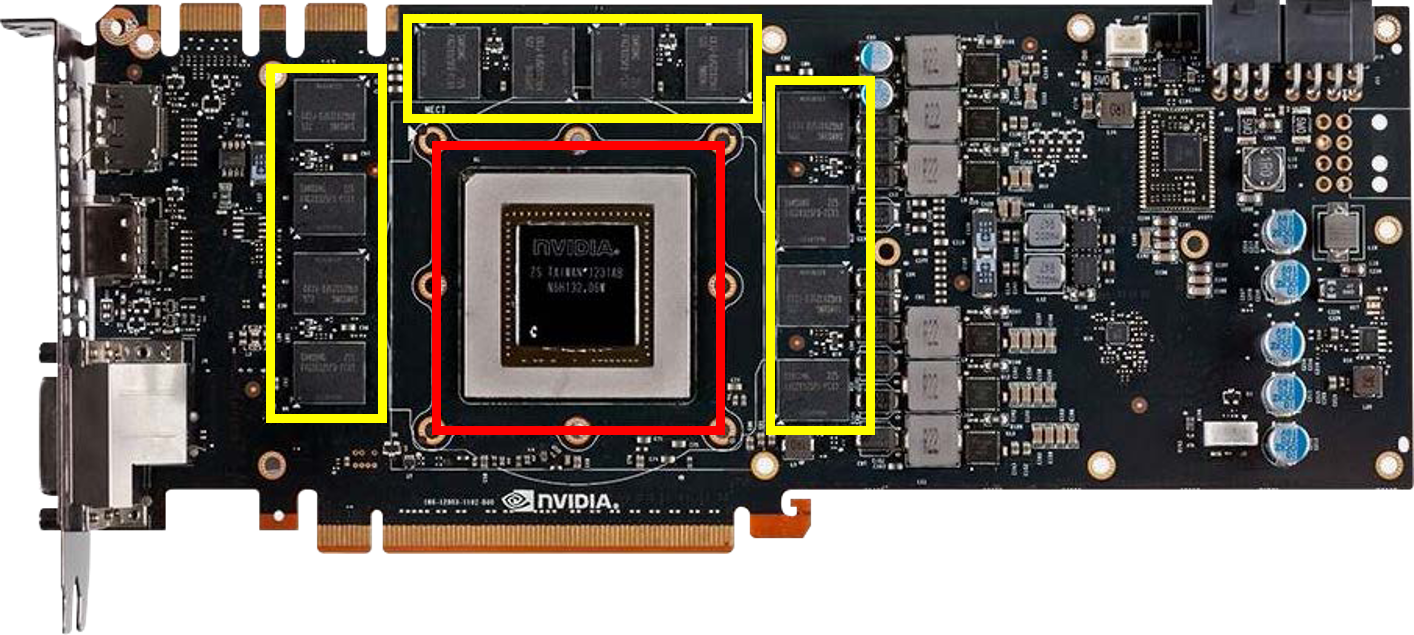
\includegraphics[width=\textwidth]{figures/gpu_intro/Kepler_box.png}
	\caption{Example of an NVIDIA GPU card. The SRAM is shown to be boxed in yellow. The GPU chip is shown to be boxed in red.}
	\label{fig:GPUarch}
\end{figure}
\begin{table}
\begin{center}
\begin{tabular}{lll}
	\toprule
	Feature 			& Tesla K40c 	& Tesla K20c 	\\ \midrule
	Memory size (GDDR5) & 12 GB 		& 5 GB 			\\
	CUDA cores 			& 2880 			& 2496 			\\
	Base clock (MHz) 	& 745 			& 732 			\\ \bottomrule
\end{tabular}
\end{center}
\caption{The computational resources available with three NVIDIA GPUs used in this thesis (1x Tesla K40c 2x Tesla K20c).}
\label{tab:gpu-resources_jeffs}
\end{table}

\section{Cuda Libraries}
CUDA isn't just a programming language, it also has many libraries that are extreemly useful that are optimized for NVIDIA GPUs.
CUDA libraries are written by NVIDIA engineers that know how to squeeze out every drop of performance out of NVIDIA GPUs.
Because ninjas are unbeatable, NVIDIA engineers are known as ninjas in the Telemetry Group at BYU.
While figuring out how to optimize a GPU kernel is extremely satisfying, GPU programmers should always search the CUDA libraries for any thing that might be useful.

Some libraries used in this Thesis are
\begin{itemize}
  \item cufft
  \item cublas
  \item cusolver
  \item cusolverSp
\end{itemize}

\section{Cuda Convolution}
An important tool to Digital Communications and Digital Signal Processing is convolution.
Time domain convolution is
\begin{align}
y(n) = \sum^{L_\text{h}-1}_{m=0} x(m) h(n-m)
	 \label{eq:simple_conv}
\end{align}
where $x(m)$, $h(n-m)$ and $y(n)$ are complex. 
While Listing \ref{code:GPUvsCPU} is a simple and good example showing how program GPUs, frankly, it is pretty boring and doesn't display the real challenges and tradeoffs of GPUs.
Listing \ref{code:convFun} shows four different ways of implementing convolution
\begin{itemize}
  \item time domain convolution in a CPU
  \item time domain convolution in a GPU using global memory
  \item time domain convolution in a GPU using shared memory
  \item frequency domain convolution in a GPU using CUDA libraries
\end{itemize}
The CPU implements Equation \eqref{eq:simple_conv} in ConvCPU directly from line $6$ to $30$.
The GPU implements time domain convolution using global memory in the GPU kernel ConvGPU.
ConvGPU on lines $32$ to $59$ is a parallel of ConvCPU.
ConvGPU implements time domain convolution by accessing global memory for any needed element of the signal and filter.

Threads accessing the same elements of the filter in global memory seems like a waste of valuable clock cycles.
The GPU kernel ConvGPUshared on lines $61$ to $96$ differs slightly from ConvGPU by making $L_\text{h}$ threads save the filter to shared memory from global memory.

Any graduate of a signal processing class knows the trade off of convolution in the time verse frequency domain.
Time domain convolution takes $\approx L_\text{s} L_\text{h}$ complex multiplies where $L_\text{s}$ is the signal length and $L_\text{h}$ is the filter length.
Frequency domain convolution takes $\approx \frac{3 N_\text{FFT}}{2} \log_2(N_\text{FFT}) + N_\text{FFT}$ complex multiplies where $N_\text{FFT}$ is the next multiple of $2$ above the convolution length $L_\text{s}+L_\text{h}-1$.

Lines $213$ to $232$ show how to do frequency domain convolution using the cuFFT library.

So the questions are:
When should I stay on the host and run my convolution on the CPU?
When should I copy my vectors to the GPU, run my convolution, then copy the vectors back to the host?
If I am going to run my convolution the GPU, when should I only use global memory?
When should I use shared memory?
When should I do convolution in the frequency domain?

The answer to all of the questions is...it depends on your signal length, filter length, CPU, GPU and memory.

The CUDA programmer can make an educated guess on which way will be fastest, but until the computations have been done in the GPU there is no definite answer.
Figure \ref{fig:CPUvsGPU} shows a comparison of computation time by varying the signal length with a set filter length.
The signal length is varied from $1$ to $~50000$ and the filter length is $186$;
The functions in \ref{code:GPUvsCPU} where ran on a NVIDIA Tesla K40c GPU.
Judging my the Figure, for signals of any significnt length, GPU convolution is much faster than CPU.
\begin{figure}
	\centering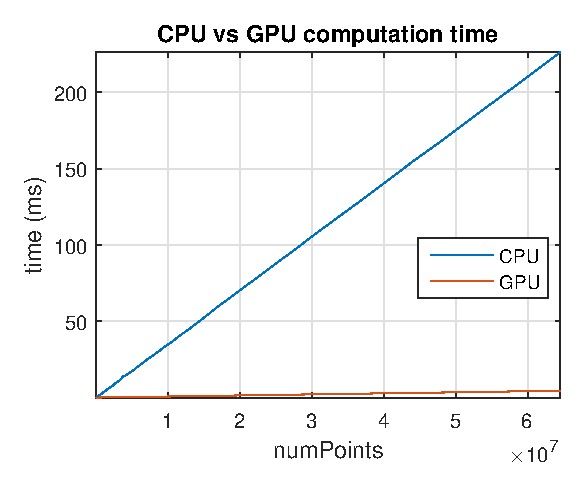
\includegraphics[width=4in]{figures/gpu_intro/CPUvsGPU.eps}
	\caption{Comparison of complex convolution in on CPU to GPU with varying signal lengths.}
	\label{fig:CPUvsGPU}
\end{figure}

Is it ever better to do convolution on the CPU rather than GPU?
Yes, but for very short signals with a $186$ tap filter.
Figure \ref{fig:CPUvsGPU_CPUtoGPU} shows when a CPU is faster than a GPU.
\begin{figure}
	\centering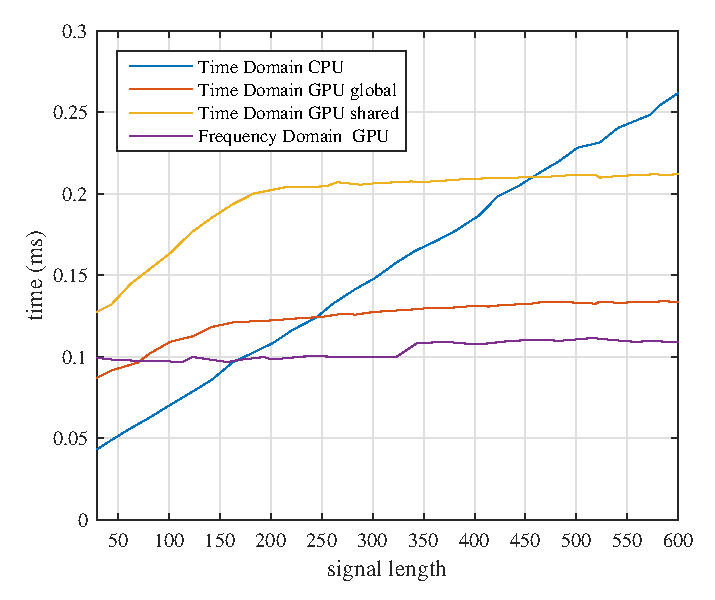
\includegraphics[width=4in]{figures/gpu_intro/CPUvsGPU_CPUtoGPU.eps}
	\caption{Plot showing when CPU convolution is faster than GPU convolution.}
	\label{fig:CPUvsGPU_CPUtoGPU}
\end{figure}

Now for the interesting question, if I am going to do convolution in the GPU, should I do time domain or frequency domain convolution?
If I do time domain convolution, should I use global or shared memory?
Figure \ref{fig:CPUvsGPU_GPUtoGPU} shows that the answer is, ``it depends''.
A good choice is to do frequency domain, but not always.
As the signal length increases, the frequency domain execution time has steps because the signal is zero padded out to the next power of 2 to leverage the Cooley-Tukey FFT algorithm \cite{Cooley-Tukey_old}.
\begin{figure}
	\centering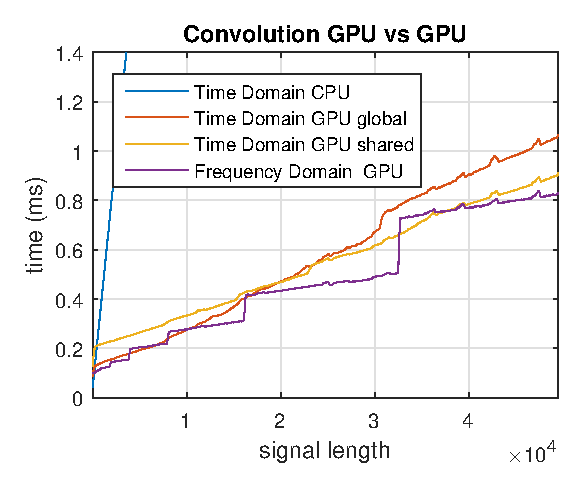
\includegraphics[width=4in]{figures/gpu_intro/CPUvsGPU_GPUtoGPU.eps}
	\caption{Plot showing trade offs with convolution in GPUs.}
	\label{fig:CPUvsGPU_GPUtoGPU}
\end{figure}

Usually, when implementing convolution, the signal and filter length is set.
If is good practice to implement convolution in the CPU and GPU in many ways to evaluate which way is best.
Choosing the signal length to be $2^{15}$ and the filter length to be $186$, Table \ref{tab:CPUvsGPUtable} shows how the different algorithms compare.
\begin{table}
\begin{center}
\begin{tabular}{lll}
	\toprule
	Algorithm 								& time (ms) \\ \midrule
	CPU time domain (ConvCPU) 				& 131.943 	\\
	GPU time domain global (ConvGPU) 		& 7.79477	\\
	GPU time domain shared (ConvGPUshared) 	& 6.77736	\\
	GPU frequency domain shared 			& 5.81085	\\ 
	\bottomrule
\end{tabular}
\end{center}
\caption{Convolution computation times with signal length $2^{15} = 32768$ and filter length $186$ on a Tesla K40c GPU.}
\label{tab:CPUvsGPUtable}
\end{table}




\section{Thread Optimization}
When first introduced to GPUs, a programmer might to tempted to launch as many threads per block possible.
But, notice in Listing \ref{code:convFun} lines $190$, $203$, $219$ and $225$ launch a minimum of $96$ threads per block and maximum of $192$ threads per block.
Running the GPU at lower occupancy leaves each thread with more resources and memory bandwidth.
If $1024$ threads per block were always launched, lighter computaion GPU kernels will be starving for memory while other thread blocks eat up the memory bandwidth.

Improving memory accesses should always be the first optimization when a GPU kernel needs to be faster.
The next step is to find the optimal number of threads per block to launch.
The number of threads per block affect the amount of resources available to each thread.
If a kernel is more computationally heavy, launching less threads per block may lead to faster execution time because threads have more resources available. 

Knowing the perfect number of threads per block to launch is challenging to calculate.
Luckily, there is a finite number of possible threads per block, $1$ to $1024$.
A simple test program could time a GPU kernel while sweeping the number of threads per block from $1$ to $1024$.
The number of threads per block with the fastest computation time is the optimal number of threads per block for that specific GPU kernel.

Most of the time the optimal number of threads per block is a multiple of $32$. 
At the lowest level of architecture, GPU do computations in \textit{warps}.
Warps are groups of $32$ threads to do every computation together in lock step.
If the number of threads per block is a non multiple of $32$, some threads in a warp will be idle and the GPU will be wasting resources.

Figure \ref{fig:threadOptimzation_ConvGPU} shows the execution time of ConvGPU while varying threads per block.
The minimum execution time is $651651$ at $128$ threads per block.










\singlespacing
\clearpage
\begin{lstlisting}[caption={CUDA code to performing complex convolution four different ways: time domain CPU, time domain GPU, time domain GPU using shared memory and frequency domain GPU.},label={code:convFun}]
#include <cufft.h>
using namespace std;
// Length of Filter (186 is a magic number)
const int LH = 186;

void ConvCPU(cufftComplex* y,cufftComplex* x,cufftComplex* h,int Lx,int Lh){
	for(int yIdx = 0; yIdx < Lx+Lh-1; yIdx++){
		cufftComplex temp;
		temp.x = 0;
		temp.y = 0;
		for(int hIdx = 0; hIdx < Lh; hIdx++){
			int xAccessIdx = yIdx-hIdx;
			if(xAccessIdx>=0 && xAccessIdx<Lx){
				// temp += x[xAccessIdx]*h[hIdx];
				// (A+jB)(C+jD) = (AC-BD) + j(AD+BC)
				float A = x[xAccessIdx].x;
				float B = x[xAccessIdx].y;
				float C = h[hIdx].x;
				float D = h[hIdx].y;
				cufftComplex complexMult;
				complexMult.x = A*C-B*D;
				complexMult.y = A*D+B*C;

				temp.x += complexMult.x;
				temp.y += complexMult.y;
			}
		}
		y[yIdx] = temp;
	}
}

__global__ void ConvGPU(cufftComplex* y,cufftComplex* x,cufftComplex* h,int Lx,int Lh){
	int yIdx = blockIdx.x*blockDim.x + threadIdx.x;
	int lastThread = Lx+Lh-1;
	// Don't access elements out of bounds
	if(yIdx >= lastThread)
		return;
	cufftComplex temp;
	temp.x = 0;
	temp.y = 0;
	for(int hIdx = 0; hIdx < Lh; hIdx++){
		int xAccessIdx = yIdx-hIdx;
		if(xAccessIdx>=0 && xAccessIdx<Lx){
			// temp += x[xAccessIdx]*h[hIdx];
			// (A+jB)(C+jD) = (AC-BD) + j(AD+BC)
			float A = x[xAccessIdx].x;
			float B = x[xAccessIdx].y;
			float C = h[hIdx].x;
			float D = h[hIdx].y;
			cufftComplex complexMult;
			complexMult.x = A*C-B*D;
			complexMult.y = A*D+B*C;

			temp.x += complexMult.x;
			temp.y += complexMult.y;
		}
		y[yIdx] = temp;
	}
}

__global__ void ConvGPUshared(cufftComplex* y,cufftComplex* x,cufftComplex* h,int Lx,int Lh){
	int yIdx = blockIdx.x*blockDim.x + threadIdx.x;
	// Be sure to read in full h_shared before checking lastThread
	// First Lh threads in thread block read h from global memory into shared memory
	__shared__ cufftComplex h_shared[LH];
	if(threadIdx.x < LH)
		h_shared[threadIdx.x] = h[threadIdx.x];
	int lastThread = Lx+Lh-1;
	// Don't access elements out of bounds
	if(yIdx >= lastThread)
		return;
	// Thread barrier, ensures threads wait until h has been read into h_shared
	__syncthreads();
	cufftComplex temp;
	temp.x = 0;
	temp.y = 0;
	for(int hIdx = 0; hIdx < Lh; hIdx++){
		int xAccessIdx = yIdx-hIdx;
		if(xAccessIdx>=0 && xAccessIdx<Lx){
			// temp += x[xAccessIdx]*h_shared[hIdx];

			// (A+jB)(C+jD) = (AC-BD) + j(AD+BC)
			float A = x[xAccessIdx].x;
			float B = x[xAccessIdx].y;
			float C = h_shared[hIdx].x;
			float D = h_shared[hIdx].y;
			cufftComplex complexMult;
			complexMult.x = A*C-B*D;
			complexMult.y = A*D+B*C;

			temp.x += complexMult.x;
			temp.y += complexMult.y;
		}
		y[yIdx] = temp;
	}
}

__global__ void PointToPointMultiply(cufftComplex* vec0, cufftComplex* vec1, int lastThread){
	int i = blockIdx.x*blockDim.x + threadIdx.x;
	// Don't access elements out of bounds
	if(i >= lastThread)
		return;
	// vec0[i] = vec0[i]*vec1[i]];
	// (A+jB)(C+jD) = (AC-BD) + j(AD+BC)
	float A = vec0[i].x;
	float B = vec0[i].y;
	float C = vec1[i].x;
	float D = vec1[i].y;
	cufftComplex complexMult;
	complexMult.x = A*C-B*D;
	complexMult.y = A*D+B*C;
	vec0[i] = complexMult;
}

__global__ void ScalarMultiply(cufftComplex* vec0, float scalar, int lastThread){
	int i = blockIdx.x*blockDim.x + threadIdx.x;
	// Don't access elements out of bounds
	if(i >= lastThread)
		return;
	cufftComplex scalarMult;
	scalarMult.x = vec0[i].x*scalar;
	scalarMult.y = vec0[i].y*scalar;
	vec0[i] = scalarMult;
}

int main(){
	int mySignalLength = pow(2,15);
	int myFilterLength = LH;
	int myConvLength   = mySignalLength + myFilterLength - 1;
	int Nfft        = pow(2, ceil(log(myConvLength)/log(2)));
	int numTreadsPerBlock;
	int numBlocks;

	cufftHandle plan;
	int n[1] = {Nfft};
	cufftPlanMany(&plan,1,n,NULL,1,1,NULL,1,1,CUFFT_C2C,1);

	// Allocate memory on host
	cufftComplex *mySignal1;
	cufftComplex *myFilter1;
	cufftComplex *myConv1;
	cufftComplex *myConv2;
	cufftComplex *myConv3;
	cufftComplex *myConv4;
	mySignal1      = (cufftComplex*) malloc(mySignalLength*sizeof(cufftComplex));
	myFilter1      = (cufftComplex*) malloc(myFilterLength*sizeof(cufftComplex));
	myConv1        = (cufftComplex*) malloc(myConvLength  *sizeof(cufftComplex));
	myConv2        = (cufftComplex*) malloc(myConvLength  *sizeof(cufftComplex));
	myConv3        = (cufftComplex*) malloc(myConvLength  *sizeof(cufftComplex));
	myConv4        = (cufftComplex*) malloc(Nfft       *sizeof(cufftComplex));
	for(int i = 0; i < mySignalLength; i++){
		mySignal1[i].x = rand()%100-50;
		mySignal1[i].y = rand()%100-50;
	}
	for(int i = 0; i < myFilterLength; i++){
		myFilter1[i].x = rand()%100-50;
		myFilter1[i].y = rand()%100-50;
	}

	// Allocate memory on device
	cufftComplex *dev_mySignal2;
	cufftComplex *dev_myFilter2;
	cufftComplex *dev_myConv2;
	cufftComplex *dev_mySignal3;
	cufftComplex *dev_myFilter3;
	cufftComplex *dev_myConv3;
	cufftComplex *dev_mySignal4;
	cufftComplex *dev_myFilter4;
	cufftComplex *dev_myConv4;
	cudaMalloc(&dev_mySignal2, mySignalLength*sizeof(cufftComplex));
	cudaMalloc(&dev_myFilter2, myFilterLength*sizeof(cufftComplex));
	cudaMalloc(&dev_myConv2,   myConvLength  *sizeof(cufftComplex));
	cudaMalloc(&dev_mySignal3, mySignalLength*sizeof(cufftComplex));
	cudaMalloc(&dev_myFilter3, myFilterLength*sizeof(cufftComplex));
	cudaMalloc(&dev_myConv3,   myConvLength  *sizeof(cufftComplex));
	cudaMalloc(&dev_mySignal4, Nfft          *sizeof(cufftComplex));
	cudaMalloc(&dev_myFilter4, Nfft          *sizeof(cufftComplex));
	cudaMalloc(&dev_myConv4,   Nfft          *sizeof(cufftComplex));

	/*---------------------------------------------------------------------------------------
                                CPU Time Domain Direct Convolution
	---------------------------------------------------------------------------------------*/
	ConvCPU(myConv1,mySignal1,myFilter1,mySignalLength,myFilterLength);

	/*---------------------------------------------------------------------------------------
                                GPU Time DomainDirect Convolution
	---------------------------------------------------------------------------------------*/
	cudaMemcpy(dev_mySignal2, mySignal1, sizeof(cufftComplex)*mySignalLength, cudaMemcpyHostToDevice);
	cudaMemcpy(dev_myFilter2, myFilter1, sizeof(cufftComplex)*myFilterLength, cudaMemcpyHostToDevice);
	numTreadsPerBlock = 128;
	numBlocks = myConvLength/numTreadsPerBlock;
	if(myConvLength % numTreadsPerBlock > 0)
		numBlocks++;
	ConvGPU<<<numBlocks, numTreadsPerBlock>>>(dev_myConv2, dev_mySignal2, dev_myFilter2, mySignalLength, myFilterLength);
	cudaMemcpy(myConv2, dev_myConv2, myConvLength*sizeof(cufftComplex), cudaMemcpyDeviceToHost);


	/*---------------------------------------------------------------------------------------
                                GPU Time Domain Convolution Using Shared Memory
	---------------------------------------------------------------------------------------*/
	cudaMemcpy(dev_mySignal3, mySignal1, sizeof(cufftComplex)*mySignalLength, cudaMemcpyHostToDevice);
	cudaMemcpy(dev_myFilter3, myFilter1, sizeof(cufftComplex)*myFilterLength, cudaMemcpyHostToDevice);
	numTreadsPerBlock = 192;
	numBlocks = myConvLength/numTreadsPerBlock;
	if(myConvLength % numTreadsPerBlock > 0)
		numBlocks++;
	ConvGPUshared<<<numBlocks, numTreadsPerBlock>>>(dev_myConv3, dev_mySignal3, dev_myFilter3, mySignalLength, myFilterLength);
	cudaMemcpy(myConv3, dev_myConv3, myConvLength*sizeof(cufftComplex), cudaMemcpyDeviceToHost);

	/*---------------------------------------------------------------------------------------
                                GPU Frequency Domain Convolution using cuFFT
	---------------------------------------------------------------------------------------*/
	cudaMemset(dev_mySignal4, 0, Nfft*sizeof(cufftComplex));
	cudaMemset(dev_myFilter4, 0, Nfft*sizeof(cufftComplex));
	cudaMemcpy(dev_mySignal4, mySignal1, sizeof(cufftComplex)*mySignalLength, cudaMemcpyHostToDevice);
	cudaMemcpy(dev_myFilter4, myFilter1, sizeof(cufftComplex)*myFilterLength, cudaMemcpyHostToDevice);
	cufftExecC2C(plan, dev_mySignal4, dev_mySignal4, CUFFT_FORWARD);
	cufftExecC2C(plan, dev_myFilter4, dev_myFilter4, CUFFT_FORWARD);
	numTreadsPerBlock = 96;
	numBlocks = Nfft/numTreadsPerBlock;
	if(Nfft % numTreadsPerBlock > 0)
		numBlocks++;
	PointToPointMultiply<<<numBlocks, numTreadsPerBlock>>>(dev_mySignal4, dev_myFilter4, Nfft);
	cufftExecC2C(plan, dev_mySignal4, dev_mySignal4, CUFFT_INVERSE);
	numTreadsPerBlock = 128;
	numBlocks = Nfft/numTreadsPerBlock;
	if(Nfft % numTreadsPerBlock > 0)
		numBlocks++;
	float scalar = 1.0/((float)Nfft);
	ScalarMultiply<<<numBlocks, numTreadsPerBlock>>>(dev_mySignal4, scalar, Nfft);
	cudaMemcpy(myConv4, dev_mySignal4, myConvLength*sizeof(cufftComplex), cudaMemcpyDeviceToHost);
	cufftDestroy(plan);

	// Free vectors on CPU
	free(mySignal1);
	free(myFilter1);
	free(myConv1);
	free(myConv2);
	free(myConv3);
	free(myConv4);

	// Free vectors on GPU
	cudaFree(dev_mySignal2);
	cudaFree(dev_myFilter2);
	cudaFree(dev_myConv2);
	cudaFree(dev_mySignal2);
	cudaFree(dev_myFilter2);
	cudaFree(dev_myConv2);
	cudaFree(dev_mySignal3);
	cudaFree(dev_myFilter3);
	cudaFree(dev_myConv3);
	cudaFree(dev_mySignal4);
	cudaFree(dev_myFilter4);
	cudaFree(dev_myConv4);

	return 0;
}
\end{lstlisting}
\doublespacing
\chapter{GPU Convolution}
\label{chap:gpu_convolution}
Convolution is one of the most important tools in any digital signal processing engineer’s toolbox. 
Convolution can be implemented in the time or frequency domain. 
%In CPUs, the number of floating point operations (flop) is the main determining factor in execution time.
%The Tesla K40c can perform 4.29 Tflops, computation is not a problem.
%The limiting factor in GPUs is the memory bandwidth.
Theory says if the given filter is ``long'', the frequency domain is the best choice.
But how long is… long? 
First we need a way to measure how computationally intensive an algorithm is. 
The number of flops is commonly used for benchmarking. 
Let the complex signal length be $N$ and the complex filter length be $L$.
Each complex multiply 
\begin{equation}
(A+jB)\times(C+jD) = (AC-BD)+j(AD+BC)
\end{equation}
is $6$ flops, $4$ multiplies and $2$ additions/subtractions.

Discrete time convolution computed in the time domain is
\begin{equation}
y(n) = \sum^{L-1}_{m=0} x(m) h(n-m).
  \label{eq:simple_conv_time}
\end{equation}
Each output element of $y(n)$ requires a $8L$ flops, $2$ flops (real and imaginary) for each term to be summed then $6$ flops for time signal and filter complex multiply.
The length of the output $\mathbf{y}$ is $N+L-1$.
The number of flops required for convolution of a given length $N$ signal and length $L$ filter is
\begin{equation}
8L(N+L-1) \text{ flops}.
\label{eq:flops_time_domain_conv}
\end{equation}

Discrete time convolution computed in the frequency domain is
\begin{equation}
\mathbf{y} = \mathscr{F}^{-1}(\mathscr{F}(\mathbf{x})\times\mathscr{F}(\mathbf{h})).
  \label{eq:simple_conv_freq}
\end{equation}
The length of the convolution, $M=N+L-1$ is the minimum point Fourier Transform possible.
It is common practice perform a next power of two above the minimum Fourier Transform to leverage the Cooley-Tukey radix 2 Fast Fourier Transform (FFT).
In the Fastest Fourier Transform in the West (FFTW) library the Cooley-Tukey radix 2 transform is used.
Each radix 2 forward or backward Fourier transform performs $5M\log_2(M)$ flops \cite{FFTW:2017,cooley1965algorithm}.
Performing convolution in the frequency domain requires
\begin{equation}
3\times5M\log_2(M)+6M \text{ flops}.
\label{eq:flops_freq_domain_conv}
\end{equation}

\section{Single Convolution}
\label{sec:cuda_convolution_single}
Figure \ref{fig:Theory186Tap_flops} compares the number of flops required for time domain verse frequency domain convolution of a $12672$ sample complex signal with a $186$ tap complex filter.
Figure \ref{fig:Theory21Tap_flops} compares the number of flops required for time domain verse frequency domain convolution of a $12672$ sample complex signal with a $21$ tap complex filter.
Appending zeros to the next power of $2$ causes the stair stepping pattern.
\begin{figure}
	\caption{Comparison of number of floating point operations (flops) required to convolve a $12672$ sample complex signal with a $186$ tap complex filter.}
	\centering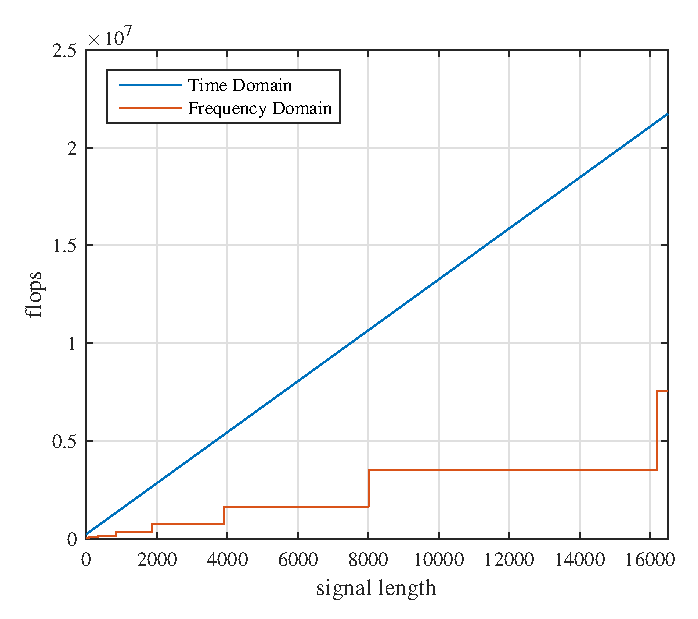
\includegraphics[width=5in]{figures/gpu_intro/Theory186Tap_flops.eps}
	\label{fig:Theory186Tap_flops}
\end{figure}
\begin{figure}
	\caption{Comparison of number of floating point operations (flops) required to convolve a $12672$ sample complex signal with a $21$ tap complex filter.}
	\centering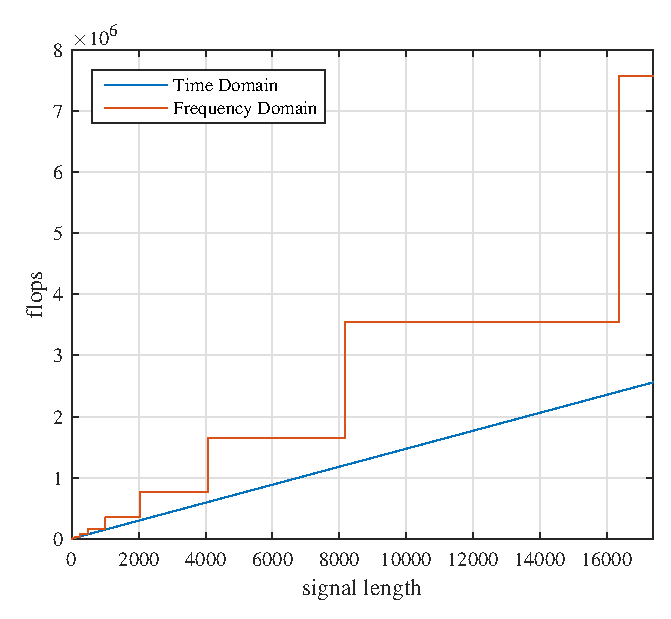
\includegraphics[width=5in]{figures/gpu_intro/Theory21Tap_flops.eps}
	\label{fig:Theory21Tap_flops}
\end{figure}


Now that we understand the number of flops required for a ``short'' filter, does the number of flops affect CPU or GPU execution time?
While Listing \ref{code:GPUvsCPU} is a simple and good example showing how program GPUs, frankly, it is pretty boring and doesn't display the real challenges and tradeoffs of GPUs.
Listing \ref{code:convFun} shows five different ways of implementing convolution:
\begin{itemize}
  \item time domain convolution in a CPU
  \item frequency domain convolution in a CPU
  \item time domain convolution in a GPU using global memory
  \item time domain convolution in a GPU using shared memory
  \item frequency domain convolution in a GPU using CUDA libraries
\end{itemize}
The CPU implements Equation \eqref{eq:simple_conv_time} in ConvCPU directly on line $209$ using a function from lines $11$ to $34$.
The CPU implements Equation \eqref{eq:simple_conv_freq} using the FFTW library on lines $214$ to $258$.
The GPU implements time domain convolution using global memory in lines $268$ to $277$.
The GPU kernel ConvGPU on lines $36$ to $64$ is a parallel version of ConvCPU.
ConvGPU implements time domain convolution by accessing global memory for every element of the signal and filter.
The GPU implements time domain convolution using shared memory in lines $283$ to $292$.
The GPU kernel ConvGPUshared on lines $67$ to $101$ is nearly identical to ConvGPU.
Threads accessing the same elements of the filter in global memory is a waste of valuable clock cycles.
ConvGPUshared pays and initial price on lines $72$ to $76$ to move $L_\text{h}$ filter coefficients from off chip global memory memory to on chip shared memory.
Finally, the GPU implements frequency domain convolution using the cuFFT library on lines $298$ to $326$.


So the questions are:
Do flops have a direct relationship to execution time on CPUs? 
Do flops have a direct relationship to execution time on GPUs? 
When is convolution in CPUs faster than GPUs?
When is it worth the initial cost to used shared memory?
When should convolution be done in the frequency domain?

The answer to all of the questions is...it depends on your signal length, filter length, CPU, GPU and memory.
A CUDA programmer can make an educated guess on which algorithm may be faster, but until all the algorithms have been implemented and timed, there is no definite answer.

To demonstrate that there is no definite answer in GPUs, 
the execution time of the code in Listing \ref{code:GPUvsCPU} was timed.
Only the CPU functions were timed for the time and frequency domain convolution on the CPU.
Each memory transfer host to device and device to host was timed for a fair comparison of GPU to CPU.
Table \ref{tab:CPUvsGPUtimingTable} shows where timing was started and stopped for each algorithm.
\begin{table}
\caption{Defining start and stop lines for timing comparison in Listing \ref{code:convFun}.}
\begin{center}
\begin{tabular}{llll}
	\toprule
	Algorithm 				& Function		& Start Line	& Stop  Line		\\ \midrule
	CPU time domain 		& ConvCPU 		& 208			& 210 				\\
	CPU frequency domain 	& FFTW 			& 213			& 259 				\\
	GPU time domain global 	& ConvGPU 		& 267			& 278				\\
	GPU time domain shared 	& ConvGPUshared & 282			& 293				\\
	GPU frequency domain 	& cuFFT			& 301			& 327				\\ 
	\bottomrule
\end{tabular}
\end{center}
\label{tab:CPUvsGPUtimingTable}
\end{table}

Figure \ref{fig:CPUvsGPU_1batch_186taps_varySignal_noMin} compares the computation time of a fixed length $186$ tap filter convolved with a varied length signal.
The execution time varies enough that the plot is messy and unreadable.
Figure \ref{fig:CPUvsGPU_1batch_186taps_varySignal} compares the same data but $15$ sample local minimums were found.
\begin{figure}
	\caption{Comparison of a complex convolution on CPU verse GPU. The signal length is varied and the filter is fixed at $186$ taps. The comparison is messy with out lower bounding.}
	\centering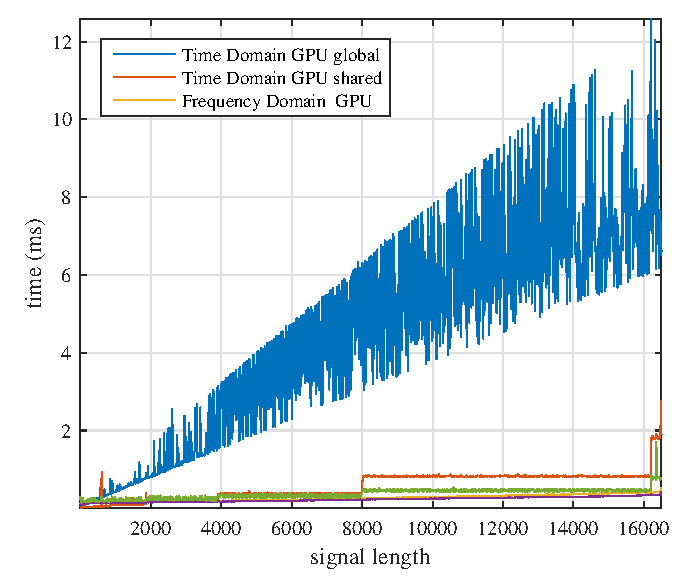
\includegraphics[width=5in]{figures/gpu_intro/CPUvsGPU_1batch_186taps_varySignal_noMin.eps}
	\label{fig:CPUvsGPU_1batch_186taps_varySignal_noMin}
\end{figure}
\begin{figure}
	\caption{Comparison of a complex convolution on CPU verse GPU. The signal length is varied and the filter is fixed at $186$ taps. A lower bound was applied by searching for a local minimums in $15$ sample width windows.}
	\centering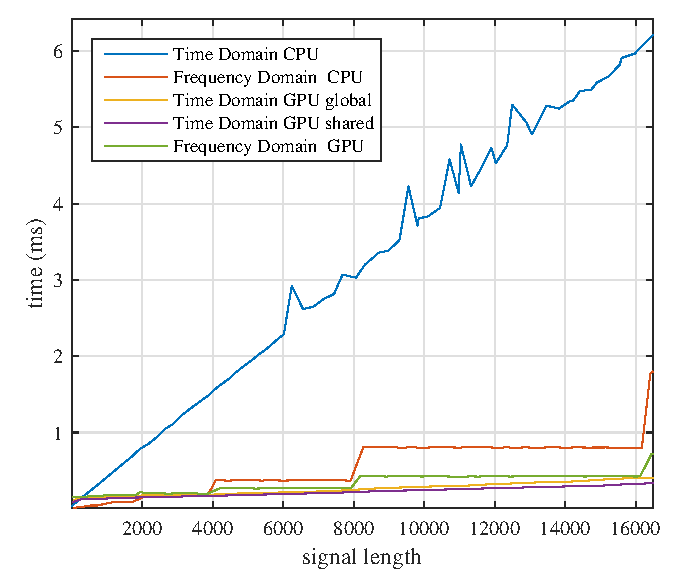
\includegraphics[width=5in]{figures/gpu_intro/CPUvsGPU_1batch_186taps_varySignal.eps}
	\label{fig:CPUvsGPU_1batch_186taps_varySignal}
\end{figure}

With the plot lower bounded, compare Figure \ref{fig:CPUvsGPU_1batch_186taps_varySignal} to Figure \ref{fig:Theory186Tap_flops}.
Does the CPU and GPU follow the same trend as the number of flops?
The CPU has the exact structure that the number of flops predicted.
The GPU does have the stair stepping from appending zeros for the frequency domain, but the time domain GPU kernels execute in less time.

The GPU execution time does not follow the same trend as the number of flops.
Why? As mentioned in Section \ref{sec:GPU_memory}, GPUs have a hanes amount of computational resources and limited memory bandwidth.
Over $90\%$ of GPU kernels are memory bandwidth limited.

To provide more proof, compare Figures \ref{fig:CPUvsGPU_1batch_21taps_varySignal} and \ref{fig:Theory21Tap_flops}.
Once again, the CPU follows the same trend as the number of flops.
The GPU also follows the number of flops trends but to a lesser extent than the CPU.
On ``short'' filters, using shared memory will perform better than using only global memory.
Using shared memory to store the short filter saves the each iteration a lot of execution time.
\begin{figure}
	\caption{Comparison of a complex convolution on CPU verse GPU. The signal length is varied and the filter is fixed at $21$ taps. A lower bound was applied by searching for a local minimums in $5$ sample width windows.}
	\centering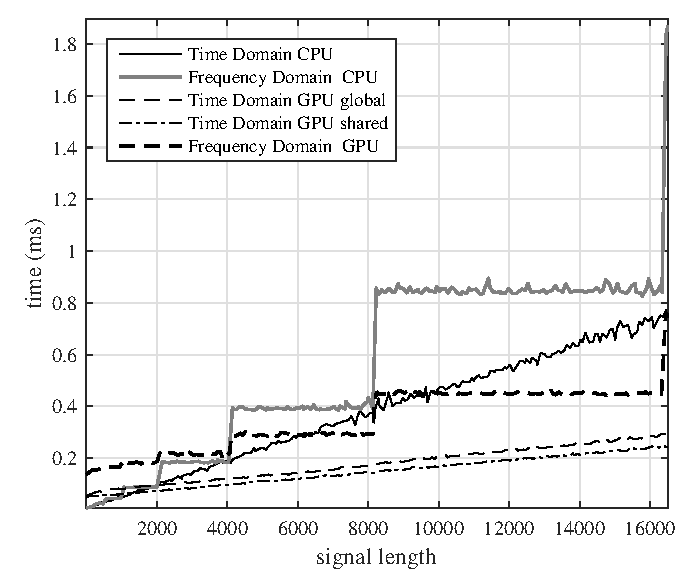
\includegraphics[width=5in]{figures/gpu_intro/CPUvsGPU_1batch_21taps_varySignal.eps}
	\label{fig:CPUvsGPU_1batch_21taps_varySignal}
\end{figure}

What if the signal length was set and the filter length was varied?
Figure \ref{fig:CPUvsGPU_1batch_12672signal_varyFilter} compares CPU to GPU execution time of a $12672$ sample signal convolved with a varying filter length.
The time domain CPU execution time is affected obviously because the number of flops increases.

Neither CPU or GPU frequency domain execution time is affected by varying filter length.
The execution time stays the same because the number of memory accesses and flops remain constant because the filter is appended with zeros to the convolution length.

The execution time of both time domain GPU convolutions are slightly affected by increasing filter length.
The number of memory accesses per output sample increase as the filter length increases.
Bottom line, the length of the signal is the largest factor as Equations \ref{eq:flops_time_domain_conv} and \ref{eq:flops_freq_domain_conv} suggest.
\begin{figure}
	\caption{Comparison of a complex convolution on CPU verse GPU. The filter length is varied and the signal is fixed at $12672$ samples. A lower bound was applied by searching for a local minimums in $3$ sample width windows.}
	\centering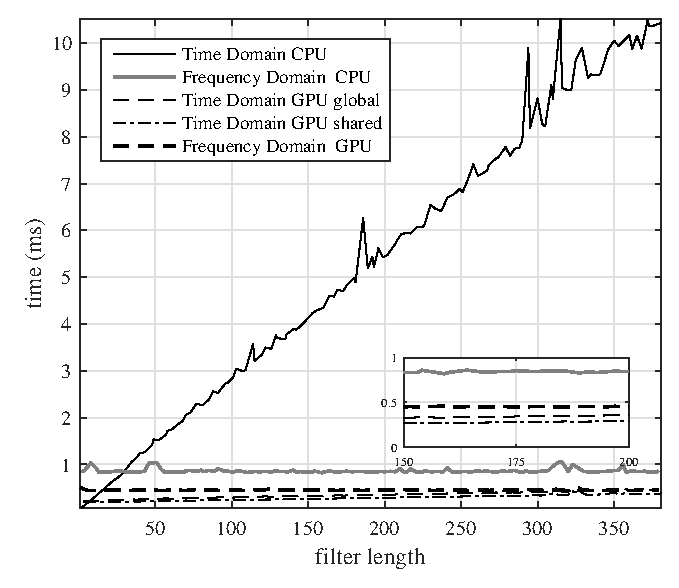
\includegraphics[width=5in]{figures/gpu_intro/CPUvsGPU_1batch_12672signal_varyFilter.eps}
	\label{fig:CPUvsGPU_1batch_12672signal_varyFilter}
\end{figure}

Conclusion, when needing implement convolution in a CPU or GPU, implement it every way possible.
Which ever way has the fastest execution time, he is your winner.
Long story short, most of the time a GPU DSP engineer is given a set length for the signal and filter.
As Figures \ref{fig:CPUvsGPU_1batch_186taps_varySignal_noMin} through \ref{fig:CPUvsGPU_1batch_12672signal_varyFilter} have shown, unless every implementation is explored, there is no way of saying which implementation will absolutely be fastest.

Table \ref{tab:CPUvsGPUtable_12672_186} shows GPU frequency domain is fastest when convolving a $12672$ sample signal with a $186$ tap filter.
Table \ref{tab:CPUvsGPUtable_12672_21} shows GPU time domain using shared is fastest when convolving a $12672$ sample signal with a $21$ tap filter.
\begin{table}
\caption{Convolution computation times with signal length $12672$ and filter length $186$ on a Tesla K40c GPU.}
\begin{center}
\begin{tabular}{lll}
	\toprule
	Algorithm 				& Function or Library		& Execution Time (ms) \\ \midrule
	CPU time domain 		& ConvCPU 					& 5.0388		\\
	CPU frequency domain 	& FFTW 						& 1.6295		\\
	GPU time domain global 	& ConvGPU 					& 0.4021		\\
	GPU time domain shared 	& ConvGPUshared 			& 0.3752		\\
	GPU frequency domain 	& cuFFT						& 0.3387		\\ 
	\bottomrule
\end{tabular}
\end{center}
\label{tab:CPUvsGPUtable_12672_186}
\end{table}
\begin{table}
\caption{Convolution computation times with signal length $12672$ and filter length $21$ on a Tesla K40c GPU.}
\begin{center}
\begin{tabular}{lll}
	\toprule
	Algorithm 				& Function or Library		& Execution Time (ms) \\ \midrule
	CPU time domain 		& ConvCPU 					& 0.6125		\\
	CPU frequency domain 	& FFTW 						& 2.5947		\\
	GPU time domain global 	& ConvGPU 					& 0.2405		\\
	GPU time domain shared 	& ConvGPUshared 			& 0.2112		\\
	GPU frequency domain 	& cuFFT						& 0.3360		\\ 
	\bottomrule
\end{tabular}
\end{center}
\label{tab:CPUvsGPUtable_12672_21}
\end{table}

\section{Batched Convolution}
In section \ref{sec:cuda_convolution_single} convolution of a single single with a single filter was studied.
Chapter blah (system overview) shows the packetized structure of the received signal.
The received signal has $3104$ packets or batches and each packet is independent of other packets.

Now that we have $3104$ signals to be convolved with $3104$ filters, how does the problem change?
Which approach to convolution will be fastest?

As the number of batches increases, does CPU and GPU execution time increase linearly?
Figure \ref{fig:CPUvsGPU_varyBatches_186taps_12672signal} shows how the execution time increases with the number of batches.
Note that no lower bounding is needed to produce clean batched processing results.
This figure shows that frequency domain convolution leverages batch processing better than time domain convolution.
No surprise CPU time and frequency domain execution time skyrockets as the number of batches increases.
The GPU handles batched processing very well because it introduces more parallelism.
\begin{figure}
	\caption{Comparison of a batched complex convolution on a CPU and GPU. The number of batches is varied while the signal and filter length is set to $12672$ and $186$.}
	\centering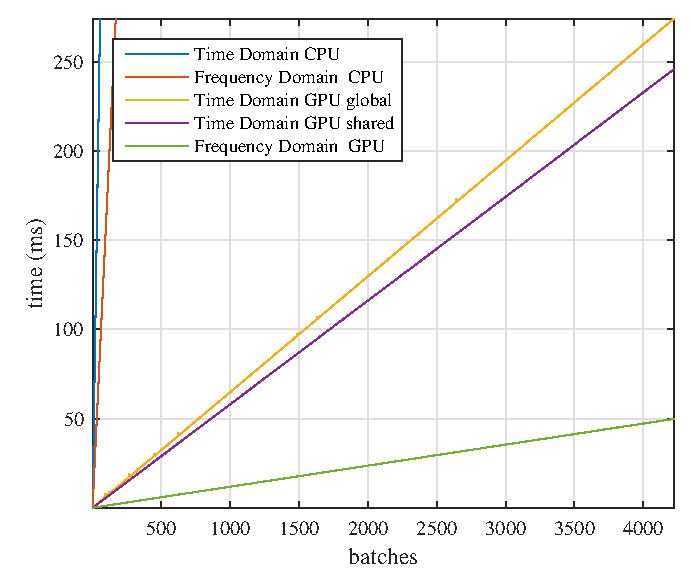
\includegraphics[width=5in]{figures/gpu_intro/CPUvsGPU_varyBatches_186taps_12672signal.eps}
	\label{fig:CPUvsGPU_varyBatches_186taps_12672signal}
\end{figure}

Judging by Figure \ref{fig:CPUvsGPU_varyBatches_186taps_12672signal}, CPU is not a contender in batched processing for fast execution times when compared to the GPU.
CPU and GPU batched processing will not be compared any further.
Listing \ref{code:batchedConvFun} shows three ways of batched convolution in CUDA
\begin{itemize}
  \item time domain convolution in a GPU using global memory
  \item time domain convolution in a GPU using shared memory
  \item frequency domain convolution in a GPU using the cuFFT library.
\end{itemize}

Now that the GPU execution time isn't being compared to the CPU, transfers between host and device will not be a factor for algorithm comparison.
Table \ref{tab:BatchedGPUtimingTable} shows how Listing \ref{code:batchedConvFun} is timed.
\begin{table}
\caption{Defining start and stop lines for timing comparison in Listing \ref{code:batchedConvFun}.}
\begin{center}
\begin{tabular}{llll}
	\toprule
	Algorithm 				& Function		& Start Line	& Stop  Line		\\ \midrule
	GPU time domain global 	& ConvGPU 		& 197			& 204				\\
	GPU time domain shared 	& ConvGPUshared & 212			& 219				\\
	GPU frequency domain 	& cuFFT			& 227			& 245				\\ 
	\bottomrule
\end{tabular}
\end{center}
\label{tab:BatchedGPUtimingTable}
\end{table}


Figure \ref{fig:CPUvsGPU_3104batch_186taps_varySignal} shows execution time for $3104$ batches of $186$ tap filters convolved with varying signal lengths.
Performing frequency domain convolution is always faster than time domain convolution because the cuFFT library is better optimized for batched processing.
Frequency domain convolution for a $12672$ sample signal takes just $36.8$ms, that is on average $0.0119$ms per batch.
Compare $0.0119$ms per batch to single batched execution time in Table \ref{tab:CPUvsGPUtable_12672_186}, one batch took $0.3387$.
Batched processing introduced a $28\times$ speed up!
\begin{figure}
	\caption{Comparison of a batched complex convolution on a GPU. The signal length is varied and the filter is fixed at $186$ taps.}
	\centering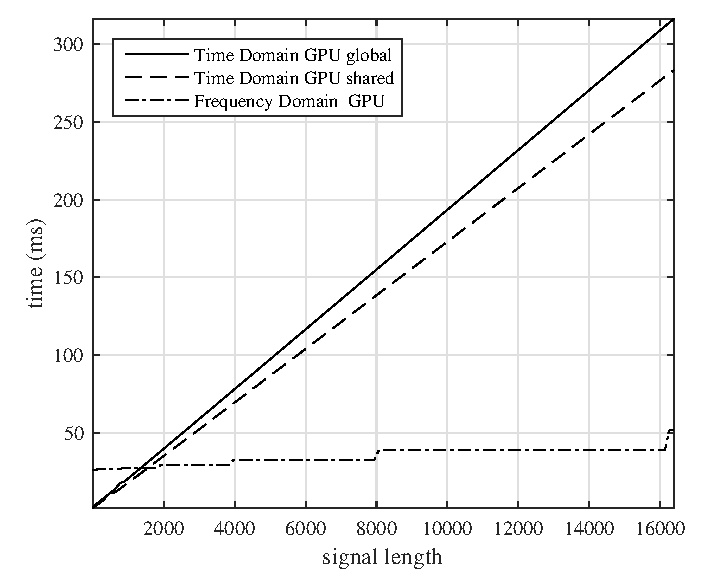
\includegraphics[width=5in]{figures/gpu_intro/CPUvsGPU_3104batch_186taps_varySignal.eps}
	\label{fig:CPUvsGPU_3104batch_186taps_varySignal}
\end{figure}

Figure \ref{fig:CPUvsGPU_3104batch_21taps_varySignal} shows execution time for $3104$ batches of $21$ tap filters convolved with varying signal lengths.
This figure exhibits the same characteristics of single batch convolution execution time shown in Figure \ref{fig:CPUvsGPU_1batch_21taps_varySignal}.
For most signal lengths, performing time domain convolution using shared memory is fastest.
\begin{figure}
	\caption{Comparison of a batched complex convolution on a GPU. The signal length is varied and the filter is fixed at $21$ taps.}
	\centering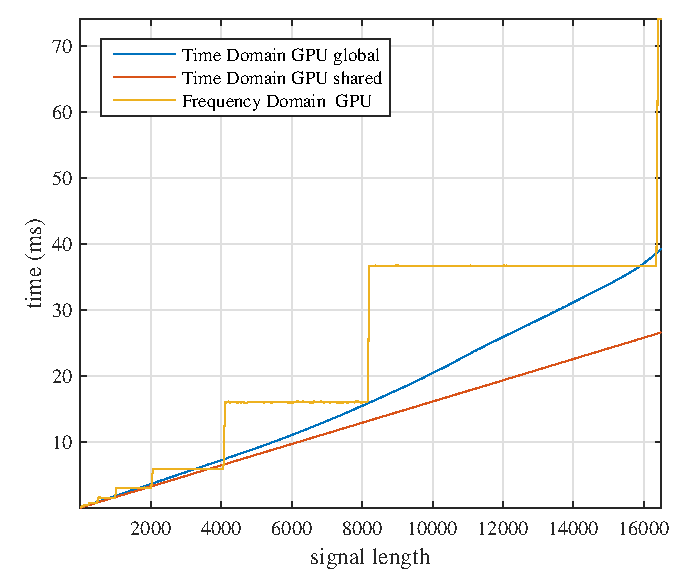
\includegraphics[width=5in]{figures/gpu_intro/CPUvsGPU_3104batch_21taps_varySignal.eps}
	\label{fig:CPUvsGPU_3104batch_21taps_varySignal}
\end{figure}

Figure \ref{fig:CPUvsGPU_3104batch_12672signal_varyFilter} shows execution time for $3104$ batches of $12672$ sample signal convolved with varying filter lengths.
This figure exhibits nearly the same characteristics of single batch convolution execution time shown in Figure \ref{fig:CPUvsGPU_1batch_12672signal_varyFilter} accept the varied filter length has no affect on execution time.
For very short filter lengths, time domain convolution using shared memory is fastest.
For longer filters , frequency domain convolution is fastest.
\begin{figure}
	\caption{Comparison of a batched complex convolution on a GPU. The signal length is varied and the filter is fixed at $21$ taps.}
	\centering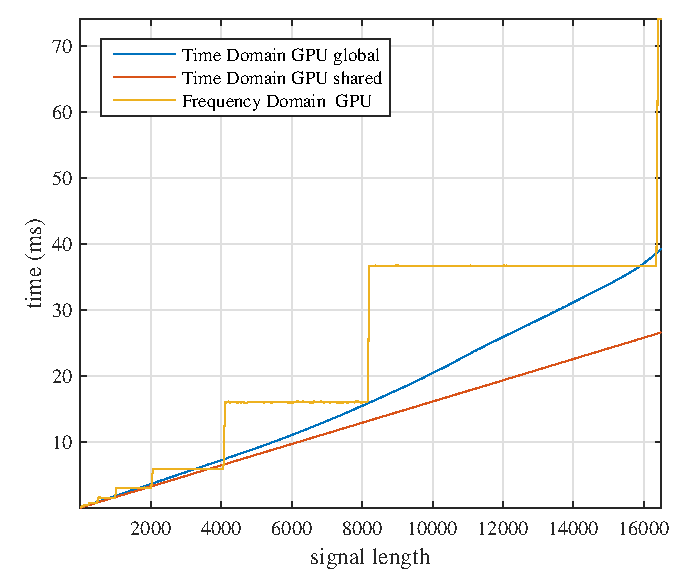
\includegraphics[width=5in]{figures/gpu_intro/CPUvsGPU_3104batch_21taps_varySignal.eps}
	\label{fig:CPUvsGPU_3104batch_21taps_varySignal}
\end{figure}

Though this section has show that in batched processing the algorithm leading to the fastest execution time still depends on signal and filter length,
one important comcept has been over looked.
Figure \ref{fig:ProcessingBlock} shows there are two filters that need to be allied to the signal. 

If convolution is implemented in the time domain, ConvGPU or ConvGPUshared must run twice.
The first call of ConvGPU or ConvGPUshared performs the convolution of the $186$ tap equalizer and $21$ detection filter.
The second call of ConvGPU or ConvGPUshared performs the convolution of the $12672$ sample signal with the  convolved $186+21-1$ tap filter.

If convolution is implemented in the frequency domain, only the GPU kernel PointToPointMultiply has to be updated.
PointToPointMultiply must be changed from two input vectors to three input vectors.
For every point the number of memory accesses increases by $1$ element and the number of flops doubles from $6$ to $12$.
An extra cuFFT call would be expected accept the detection filter in Figure \ref{fig:ProcessingBlock} constant.
The FFT of the detection filter can be calculated and stored at initialization.

Table \ref{tab:Batched_CPUvsGPUtable_12672_186} shows the batched convolution execution time for a $12672$ sample signal and $186$ tap filter.
Table \ref{tab:Batched_CPUvsGPUtable_12672_21} shows the batched convolution execution time for a $12672$ sample signal and $21$ tap filter.
Table \ref{tab:Batched_CPUvsGPUtable_12672_21_186} shows the batched cascaded convolution execution time for a $12672$ sample signal with $21$ and $186$ tap filters.
\begin{table}
\caption{Batched convolution execution times with for a $12672$ sample signal and $186$ tap filter on a Tesla K40c GPU.}
\begin{center}
\begin{tabular}{lll}
	\toprule
	Algorithm 				& Function or Library		& Execution Time (ms) \\ \midrule
	GPU time domain global 	& ConvGPU 					& 201.29		\\
	GPU time domain shared 	& ConvGPUshared 			& 180.272		\\
	GPU frequency domain 	& cuFFT						& 36.798 		\\ 
	\bottomrule
\end{tabular}
\end{center}
\label{tab:Batched_CPUvsGPUtable_12672_186}
\end{table}
\begin{table}
\caption{Batched convolution execution times with for a $12672$ sample signal and $21$ tap filter on a Tesla K40c GPU.}
\begin{center}
\begin{tabular}{lll}
	\toprule
	Algorithm 				& Function or Library		& Execution Time (ms) \\ \midrule
	GPU time domain global 	& ConvGPU 					& 27.642		\\
	GPU time domain shared 	& ConvGPUshared 			& 20.4287		\\
	GPU frequency domain 	& cuFFT						& 36.7604		\\ 
	\bottomrule
\end{tabular}
\end{center}
\label{tab:Batched_CPUvsGPUtable_12672_21}
\end{table}
\begin{table}
\caption{Batched convolution execution times with for a $12672$ sample signal and $206$ tap filter on a Tesla K40c GPU.}
\begin{center}
\begin{tabular}{lll}
	\toprule
	Algorithm 				& Function or Library		& Execution Time (ms) \\ \midrule
	GPU time domain global 	& ConvGPU 					& 223.064		\\
	GPU time domain shared 	& ConvGPUshared 			& 199.844		\\
	GPU frequency domain 	& cuFFT						& 36.7704		\\ 
	\bottomrule
\end{tabular}
\end{center}
\label{tab:Batched_CPUvsGPUtable_12672_206}
\end{table}
\begin{table}
\caption{Batched convolution execution times with for a $12672$ sample signal and cascaded $21$ and $186$ tap filter on a Tesla K40c GPU.}
\begin{center}
\begin{tabular}{lll}
	\toprule
	Algorithm 				& Function or Library		& Execution Time (ms) \\ \midrule
	GPU time domain global 	& ConvGPU 					& 223.307		\\
	GPU time domain shared 	& ConvGPUshared 			& 200.018		\\
	GPU frequency domain 	& cuFFT						& 39.0769		\\ 
	\bottomrule
\end{tabular}
\end{center}
\label{tab:Batched_CPUvsGPUtable_12672_21_186}
\end{table}

Tables \ref{tab:Batched_CPUvsGPUtable_12672_186} and \ref{tab:Batched_CPUvsGPUtable_12672_21} agree with Figures \ref{fig:CPUvsGPU_3104batch_21taps_varySignal} and \ref{fig:CPUvsGPU_3104batch_186taps_varySignal}.
Time domain convolution is faster with a short $21$ tap filter but frequency domain convolution is faster with a long $186$ tap filter.

\begin{figure}
	\caption{Two ways to convolve the signal $\mathbf{r}$ with the $186$ tap filter $\mathbf{c}$ and $21$ tap filter $\mathbf{d}$.}
	\centering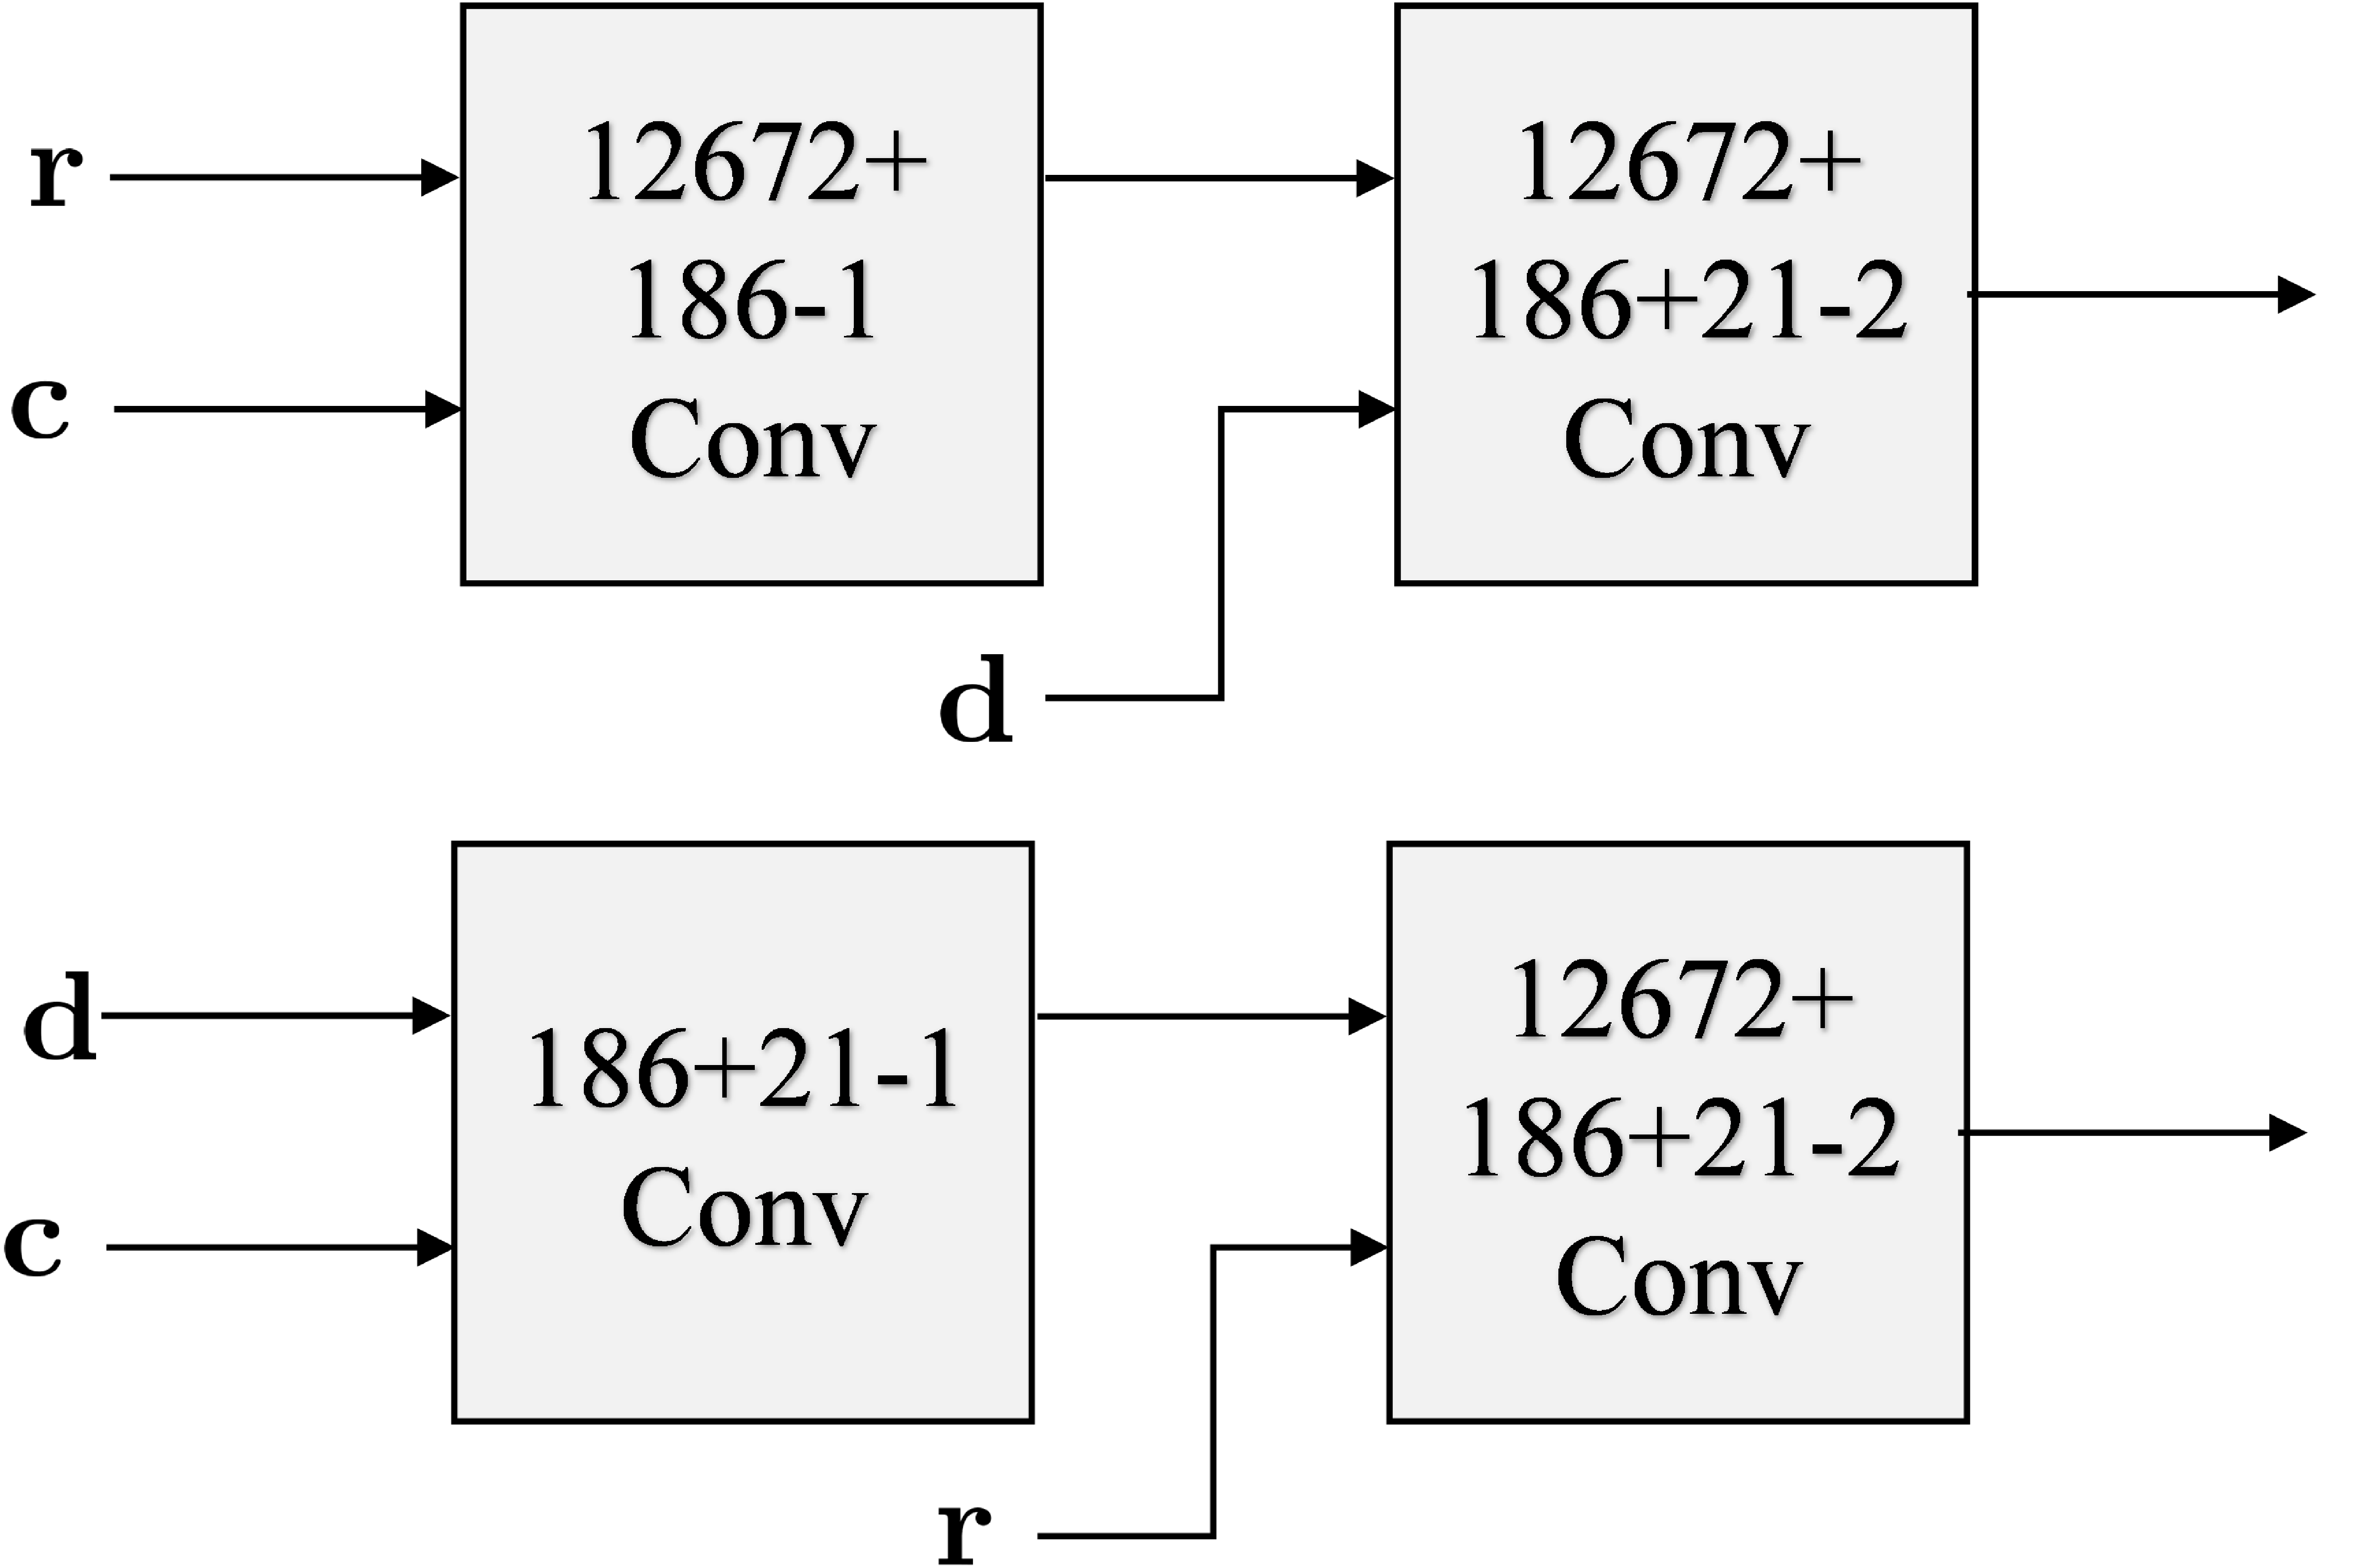
\includegraphics[width=5.01in/100*55]{figures/gpu_intro/twoWaysToConv.pdf}
	\label{fig:twoWaysToConv}
\end{figure}
Figure \ref{fig:twoWaysToConv} shows two ways to cascade the signal $\mathbf{r}$ though two filters.
Rather than applying both filters to the signal, compute a shorter convolution of the $186$ and $21$ tap filters then apply the $186+21-1$ tap result to the signal.

Table \ref{tab:Batched_CPUvsGPUtable_12672_21_186} shows the execution time of implementing cascaded filters, convolving the $21$ and $186$ tap filters is extremely fast in the GPU.
It only costs $2.3165$ms to apply an extra filter in the frequency domain.
It costs $22.0170$ms and $19.7460$ms to apply an extra filter in the time domain because the cascaded filter is now $206$ taps rather than $186$.
Table \ref{tab:Batched_CPUvsGPUtable_12672_206} confirms it costs an extra $20$ms or so to apply a $206$ vs $186$ tap filter.







%%CPUvsGPU_3104batch_21taps_186taps_cascade_varySignal








\section{Cuda Convolution}
Convolution is one of the most important tools in any digital signal processing engineer’s toolbox. 
Convolution can be implemented in the time or frequency domain. 
Theory says if the given filter is ``long'', the frequency domain is the best choice.
But how long is… long? 
First we need a way to measure how computationally intensive an algorithm is. 
The number of floating point operations (flops) is commonly used for benchmarking. 
Let the complex signal length be $N$ and the complex filter length be $L$.
Each complex multiply 
\begin{equation}
(A+jB)\times(C+jD) = (AC-BD)+j(AD+BC)
\end{equation}
is $6$ flops, $4$ multiplies and $2$ additions/subtractions.

Discrete time convolution computed in the time domain is
\begin{equation}
y(n) = \sum^{L-1}_{m=0} x(m) h(n-m).
  \label{eq:simple_conv_time}
\end{equation}
Each output element of $y(n)$ requires a $8L$ flops, $2$ flops (real and imaginary) for each term to be summed then $6$ flops for time signal and filter complex multiply.
The length of the output $\mathbf{y}$ is $N+L-1$.
The number of flops required for convolution of a given length $N$ signal and length $L$ filter is
\begin{equation}
8L(N+L-1) \text{ flops}.
\label{eq:flops_time_domain_conv}
\end{equation}

Discrete time convolution computed in the frequency domain is
\begin{equation}
\mathbf{y} = \mathscr{F}^{-1}(\mathscr{F}(\mathbf{x})\times\mathscr{F}(\mathbf{h})).
  \label{eq:simple_conv_freq}
\end{equation}
The length of the convolution, $M=N+L-1$ is the minimum point Fourier Transform possible.
It is common practice perform a next power of two above the minimum Fourier Transform to leverage the Cooley-Tukey radix 2 Fast Fourier Transform (FFT).
In the Fastest Fourier Transform in the West (FFTW) library the Cooley-Tukey radix 2 transform is used.
Each radix 2 forward or backward Fourier transform performs $5M\log_2(M)$ flops \cite{FFTW:2017,cooley1965algorithm}.
Performing convolution in the frequency domain requires
\begin{equation}
3\times5M\log_2(M)+6M \text{ flops}.
\label{eq:flops_freq_domain_conv}
\end{equation}

\section{Single Convolution}
\label{sec:cuda_convolution_single}
Figure \ref{fig:Theory186Tap_flops} compares the number of flops required for time domain verse frequency domain convolution of a $12672$ sample complex signal with a $186$ tap complex filter.
Figure \ref{fig:Theory21Tap_flops} compares the number of flops required for time domain verse frequency domain convolution of a $12672$ sample complex signal with a $21$ tap complex filter.
Appending zeros to the next power of $2$ causes the stair stepping pattern.
\begin{figure}
	\caption{Comparison of number of floating point operations (flops) required to convolve a $12672$ sample complex signal with a $186$ tap complex filter.}
	\centering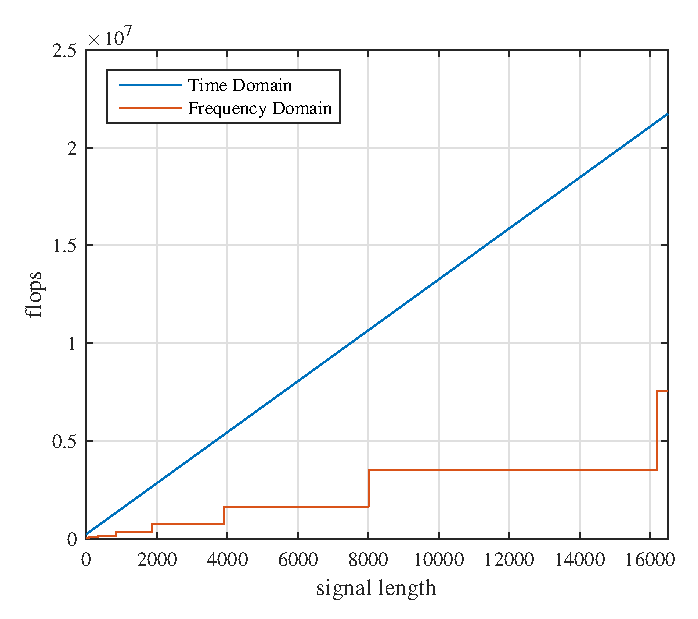
\includegraphics[width=5in]{figures/gpu_intro/Theory186Tap_flops.eps}
	\label{fig:Theory186Tap_flops}
\end{figure}
\begin{figure}
	\caption{Comparison of number of floating point operations (flops) required to convolve a $12672$ sample complex signal with a $21$ tap complex filter.}
	\centering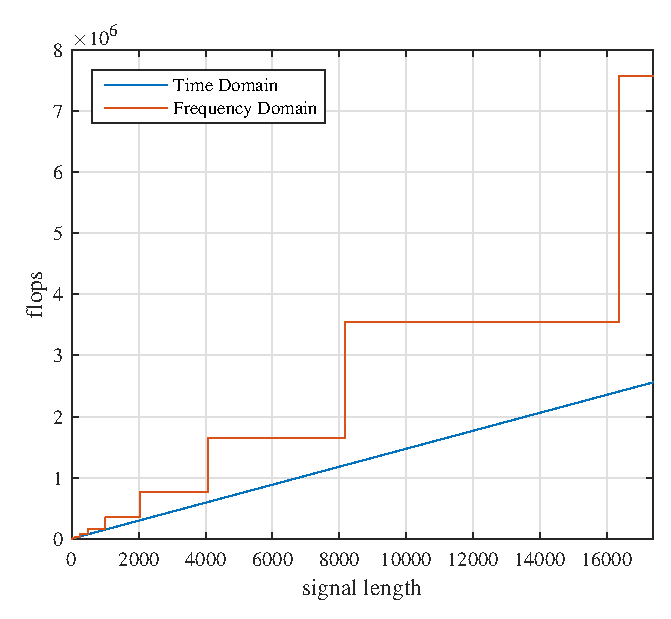
\includegraphics[width=5in]{figures/gpu_intro/Theory21Tap_flops.eps}
	\label{fig:Theory21Tap_flops}
\end{figure}


Now that we understand the number of flops required for a ``short'' filter, does the number of flops affect CPU or GPU execution time?
While Listing \ref{code:GPUvsCPU} is a simple and good example showing how program GPUs, frankly, it is pretty boring and doesn't display the real challenges and tradeoffs of GPUs.
Listing \ref{code:convFun} shows five different ways of implementing convolution:
\begin{itemize}
  \item time domain convolution in a CPU
  \item frequency domain convolution in a CPU
  \item time domain convolution in a GPU using global memory
  \item time domain convolution in a GPU using shared memory
  \item frequency domain convolution in a GPU using CUDA libraries
\end{itemize}
The CPU implements Equation \eqref{eq:simple_conv_time} in ConvCPU directly on line $209$ using a function from lines $11$ to $34$.
The CPU implements Equation \eqref{eq:simple_conv_freq} using the FFTW library on lines $214$ to $258$.
The GPU implements time domain convolution using global memory in lines $268$ to $277$.
The GPU kernel ConvGPU on lines $36$ to $64$ is a parallel version of ConvCPU.
ConvGPU implements time domain convolution by accessing global memory for every element of the signal and filter.
The GPU implements time domain convolution using shared memory in lines $283$ to $292$.
The GPU kernel ConvGPUshared on lines $67$ to $101$ is nearly identical to ConvGPU.
Threads accessing the same elements of the filter in global memory is a waste of valuable clock cycles.
ConvGPUshared pays and initial price on lines $72$ to $76$ to move $L_\text{h}$ filter coefficients from off chip global memory memory to on chip shared memory.
Finally, the GPU implements frequency domain convolution using the cuFFT library on lines $298$ to $326$.


So the questions are:
Do flops have a direct relationship to execution time on CPUs? 
Do flops have a direct relationship to execution time on GPUs? 
When is convolution in CPUs faster than GPUs?
When is it worth the initial cost to used shared memory?
When should convolution be done in the frequency domain?

The answer to all of the questions is...it depends on your signal length, filter length, CPU, GPU and memory.
A CUDA programmer can make an educated guess on which algorithm may be faster, but until all the algorithms have been implemented and timed, there is no definite answer.

To demonstrate that there is no definite answer in GPUs, 
the execution time of the code in Listing \ref{code:GPUvsCPU} was timed.
Only the CPU functions were timed for the time and frequency domain convolution on the CPU.
Each memory transfer host to device and device to host was timed for a fair comparison of GPU to CPU.
Table \ref{tab:CPUvsGPUtimingTable} shows where timing was started and stopped for each algorithm.
\begin{table}
\caption{Defining start and stop lines for timing comparison in Listing \ref{code:convFun}.}
\begin{center}
\begin{tabular}{llll}
	\toprule
	Algorithm 				& Function		& Start Line	& Stop  Line		\\ \midrule
	CPU time domain 		& ConvCPU 		& 208			& 210 				\\
	CPU frequency domain 	& FFTW 			& 213			& 259 				\\
	GPU time domain global 	& ConvGPU 		& 267			& 278				\\
	GPU time domain shared 	& ConvGPUshared & 282			& 293				\\
	GPU frequency domain 	& cuFFT			& 301			& 327				\\ 
	\bottomrule
\end{tabular}
\end{center}
\label{tab:CPUvsGPUtimingTable}
\end{table}

Figure \ref{fig:CPUvsGPU_1batch_186taps_varySignal_noMin} compares the computation time of a fixed length $186$ tap filter convolved with a varied length signal.
The execution time varies enough that the plot is messy and unreadable.
Figure \ref{fig:CPUvsGPU_1batch_186taps_varySignal} compares the same data but $15$ sample local minimums were found.
\begin{figure}
	\caption{Comparison of a complex convolution on CPU verse GPU. The signal length is varied and the filter is fixed at $186$ taps. The comparison is messy with out lower bounding.}
	\centering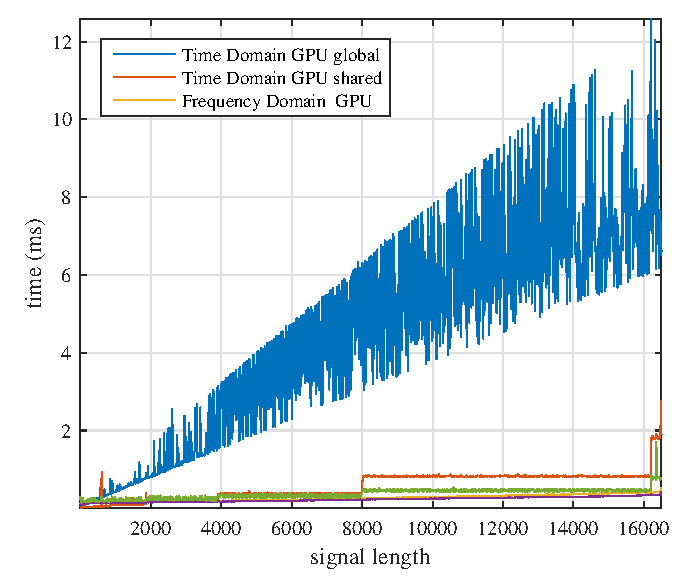
\includegraphics[width=5in]{figures/gpu_intro/CPUvsGPU_1batch_186taps_varySignal_noMin.eps}
	\label{fig:CPUvsGPU_1batch_186taps_varySignal_noMin}
\end{figure}
\begin{figure}
	\caption{Comparison of a complex convolution on CPU verse GPU. The signal length is varied and the filter is fixed at $186$ taps. A lower bound was applied by searching for a local minimums in $15$ sample width windows.}
	\centering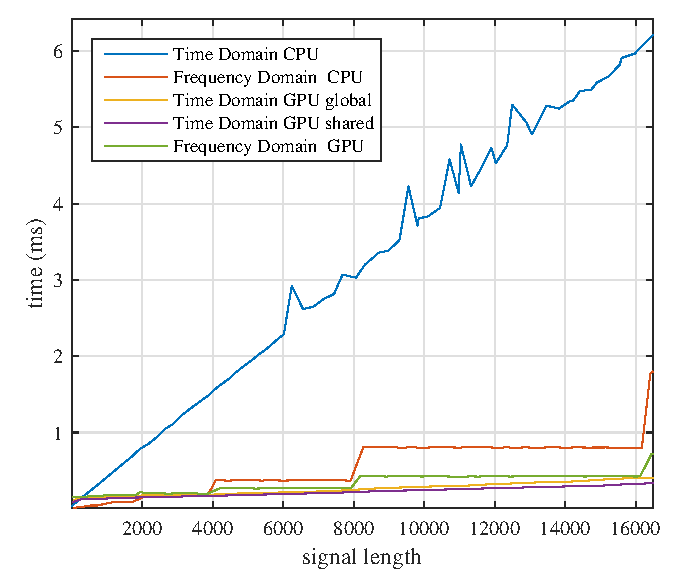
\includegraphics[width=5in]{figures/gpu_intro/CPUvsGPU_1batch_186taps_varySignal.eps}
	\label{fig:CPUvsGPU_1batch_186taps_varySignal}
\end{figure}

With the plot lower bounded, compare Figure \ref{fig:CPUvsGPU_1batch_186taps_varySignal} to Figure \ref{fig:Theory186Tap_flops}.
Does the CPU and GPU follow the same trend as the number of flops?
The CPU has the exact structure that the number of flops predicted.
The GPU does have the stair stepping from appending zeros for the frequency domain, but the time domain GPU kernels execute in less time.

The GPU execution time does not follow the same trend as the number of flops.
Why? As mentioned in Section \ref{sec:GPU_memory}, GPUs have a hanes amount of computational resources and limited memory bandwidth.
Over $90\%$ of GPU kernels are memory bandwidth limited.

To provide more proof, compare Figures \ref{fig:CPUvsGPU_1batch_21taps_varySignal} and \ref{fig:Theory21Tap_flops}.
Once again, the CPU follows the same trend as the number of flops.
The GPU also follows the number of flops trends but to a lesser extent than the CPU.
On ``short'' filters, using shared memory will perform better than using only global memory.
Using shared memory to store the short filter saves the each iteration a lot of execution time.
\begin{figure}
	\caption{Comparison of a complex convolution on CPU verse GPU. The signal length is varied and the filter is fixed at $21$ taps. A lower bound was applied by searching for a local minimums in $5$ sample width windows.}
	\centering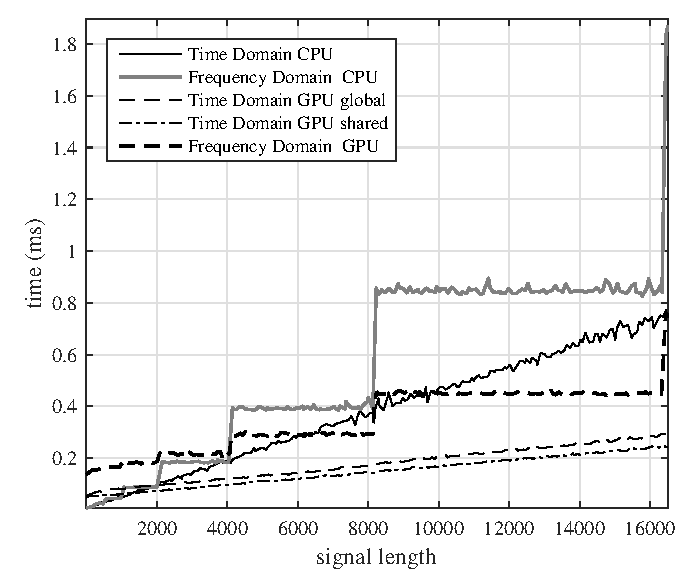
\includegraphics[width=5in]{figures/gpu_intro/CPUvsGPU_1batch_21taps_varySignal.eps}
	\label{fig:CPUvsGPU_1batch_21taps_varySignal}
\end{figure}

What if the signal length was set and the filter length was varied?
Figure \ref{fig:CPUvsGPU_1batch_12672signal_varyFilter} compares CPU to GPU execution time of a $12672$ sample signal convolved with a varying filter length.
The time domain CPU execution time is affected obviously because the number of flops increases.

Neither CPU or GPU frequency domain execution time is affected by varying filter length.
The execution time stays the same because the number of memory accesses and flops remain constant because the filter is appended with zeros to the convolution length.

The execution time of both time domain GPU convolutions are slightly affected by increasing filter length.
The number of memory accesses per output sample increase as the filter length increases.
Bottom line, the length of the signal is the largest factor as Equations \ref{eq:flops_time_domain_conv} and \ref{eq:flops_freq_domain_conv} suggest.
\begin{figure}
	\caption{Comparison of a complex convolution on CPU verse GPU. The filter length is varied and the signal is fixed at $12672$ samples. A lower bound was applied by searching for a local minimums in $3$ sample width windows.}
	\centering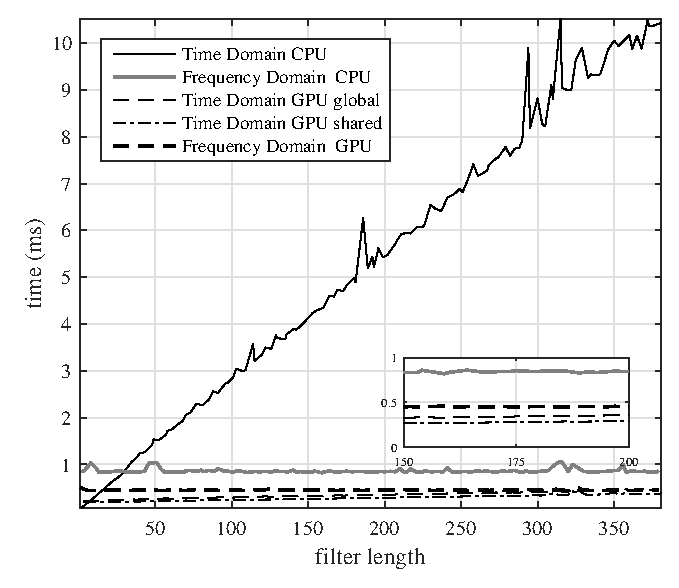
\includegraphics[width=5in]{figures/gpu_intro/CPUvsGPU_1batch_12672signal_varyFilter.eps}
	\label{fig:CPUvsGPU_1batch_12672signal_varyFilter}
\end{figure}

Conclusion, when needing implement convolution in a CPU or GPU, implement it every way possible.
Which ever way has the fastest execution time, he is your winner.
Long story short, most of the time a GPU DSP engineer is given a set length for the signal and filter.
As Figures \ref{fig:CPUvsGPU_1batch_186taps_varySignal_noMin} through \ref{fig:CPUvsGPU_1batch_12672signal_varyFilter} have shown, unless every implementation is explored, there is no way of saying which implementation will absolutely be fastest.

Table \ref{tab:CPUvsGPUtable_12672_186} shows GPU frequency domain is fastest when convolving a $12672$ sample signal with a $186$ tap filter.
Table \ref{tab:CPUvsGPUtable_12672_21} shows GPU time domain using shared is fastest when convolving a $12672$ sample signal with a $21$ tap filter.
\begin{table}
\caption{Convolution computation times with signal length $12672$ and filter length $186$ on a Tesla K40c GPU.}
\begin{center}
\begin{tabular}{lll}
	\toprule
	Algorithm 				& Function or Library		& Execution Time (ms) \\ \midrule
	CPU time domain 		& ConvCPU 					& 5.0388		\\
	CPU frequency domain 	& FFTW 						& 1.6295		\\
	GPU time domain global 	& ConvGPU 					& 0.4021		\\
	GPU time domain shared 	& ConvGPUshared 			& 0.3752		\\
	GPU frequency domain 	& cuFFT						& 0.3387		\\ 
	\bottomrule
\end{tabular}
\end{center}
\label{tab:CPUvsGPUtable_12672_186}
\end{table}
\begin{table}
\caption{Convolution computation times with signal length $12672$ and filter length $21$ on a Tesla K40c GPU.}
\begin{center}
\begin{tabular}{lll}
	\toprule
	Algorithm 				& Function or Library		& Execution Time (ms) \\ \midrule
	CPU time domain 		& ConvCPU 					& 0.6125		\\
	CPU frequency domain 	& FFTW 						& 2.5947		\\
	GPU time domain global 	& ConvGPU 					& 0.2405		\\
	GPU time domain shared 	& ConvGPUshared 			& 0.2112		\\
	GPU frequency domain 	& cuFFT						& 0.3360		\\ 
	\bottomrule
\end{tabular}
\end{center}
\label{tab:CPUvsGPUtable_12672_21}
\end{table}

\section{Batched Convolution}
In section \ref{sec:cuda_convolution_single} convolution of a single single with a single filter was studied.
Chapter blah (system overview) shows the packetized structure of the received signal.
The received signal has $3104$ packets or batches and each packet is independent of other packets.

Now that we have $3104$ signals to be convolved with $3104$ filters, how does the problem change?
Which approach to convolution will be fastest?

As the number of batches increases, does CPU and GPU execution time increase linearly?
Figure \ref{fig:CPUvsGPU_varyBatches_186taps_12672signal} shows how the execution time increases with the number of batches.
Note that no lower bounding is needed to produce clean batched processing results.
This figure shows that frequency domain convolution leverages batch processing better than time domain convolution.
No surprise CPU time and frequency domain execution time skyrockets as the number of batches increases.
The GPU handles batched processing very well because it introduces more parallelism.
\begin{figure}
	\caption{Comparison of a batched complex convolution on a CPU and GPU. The number of batches is varied while the signal and filter length is set to $12672$ and $186$.}
	\centering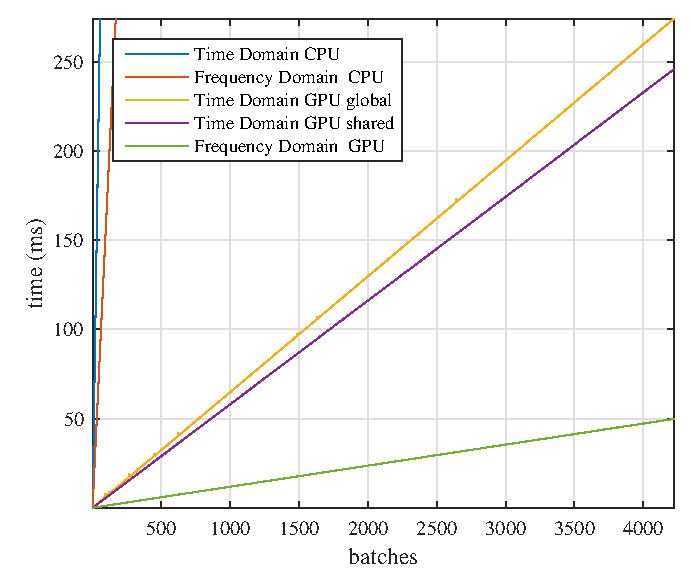
\includegraphics[width=5in]{figures/gpu_intro/CPUvsGPU_varyBatches_186taps_12672signal.eps}
	\label{fig:CPUvsGPU_varyBatches_186taps_12672signal}
\end{figure}

Judging by Figure \ref{fig:CPUvsGPU_varyBatches_186taps_12672signal}, CPU is not a contender in batched processing for fast execution times when compared to the GPU.
CPU and GPU batched processing will not be compared any further.
Listing \ref{code:batchedConvFun} shows three ways of batched convolution in CUDA
\begin{itemize}
  \item time domain convolution in a GPU using global memory
  \item time domain convolution in a GPU using shared memory
  \item frequency domain convolution in a GPU using the cuFFT library.
\end{itemize}

Now that the GPU execution time isn't being compared to the CPU, transfers between host and device will not be a factor for algorithm comparison.
Table \ref{tab:BatchedGPUtimingTable} shows how Listing \ref{code:batchedConvFun} is timed.
\begin{table}
\caption{Defining start and stop lines for timing comparison in Listing \ref{code:batchedConvFun}.}
\begin{center}
\begin{tabular}{llll}
	\toprule
	Algorithm 				& Function		& Start Line	& Stop  Line		\\ \midrule
	GPU time domain global 	& ConvGPU 		& 197			& 204				\\
	GPU time domain shared 	& ConvGPUshared & 212			& 219				\\
	GPU frequency domain 	& cuFFT			& 227			& 245				\\ 
	\bottomrule
\end{tabular}
\end{center}
\label{tab:BatchedGPUtimingTable}
\end{table}


Figure \ref{fig:CPUvsGPU_3104batch_186taps_varySignal} shows execution time for $3104$ batches of $186$ tap filters convolved with varying signal lengths.
Performing frequency domain convolution is always faster than time domain convolution because the cuFFT library is better optimized for batched processing.
Frequency domain convolution for a $12672$ sample signal takes just $36.8$ms, that is on average $0.0119$ms per batch.
Compare $0.0119$ms per batch to single batched execution time in Table \ref{tab:CPUvsGPUtable_12672_186}, one batch took $0.3387$.
Batched processing introduced a $28\times$ speed up!
\begin{figure}
	\caption{Comparison of a batched complex convolution on a GPU. The signal length is varied and the filter is fixed at $186$ taps.}
	\centering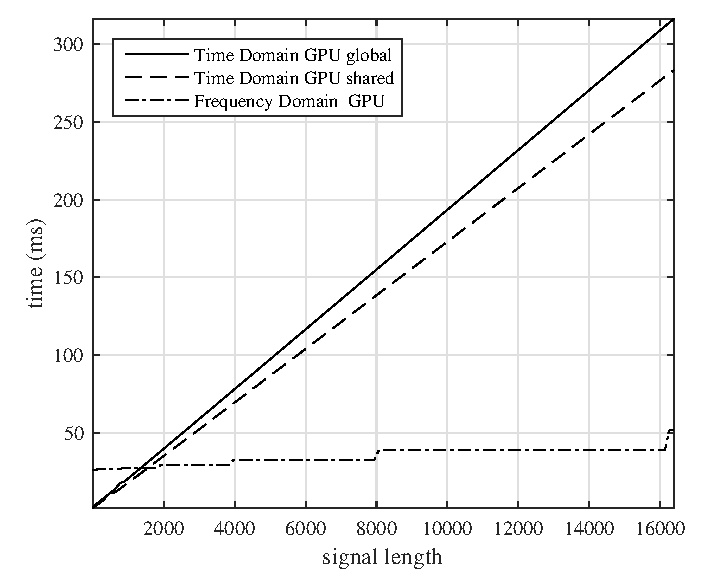
\includegraphics[width=5in]{figures/gpu_intro/CPUvsGPU_3104batch_186taps_varySignal.eps}
	\label{fig:CPUvsGPU_3104batch_186taps_varySignal}
\end{figure}

Figure \ref{fig:CPUvsGPU_3104batch_21taps_varySignal} shows execution time for $3104$ batches of $21$ tap filters convolved with varying signal lengths.
This figure exhibits the same characteristics of single batch convolution execution time shown in Figure \ref{fig:CPUvsGPU_1batch_21taps_varySignal}.
For most signal lengths, performing time domain convolution using shared memory is fastest.
\begin{figure}
	\caption{Comparison of a batched complex convolution on a GPU. The signal length is varied and the filter is fixed at $21$ taps.}
	\centering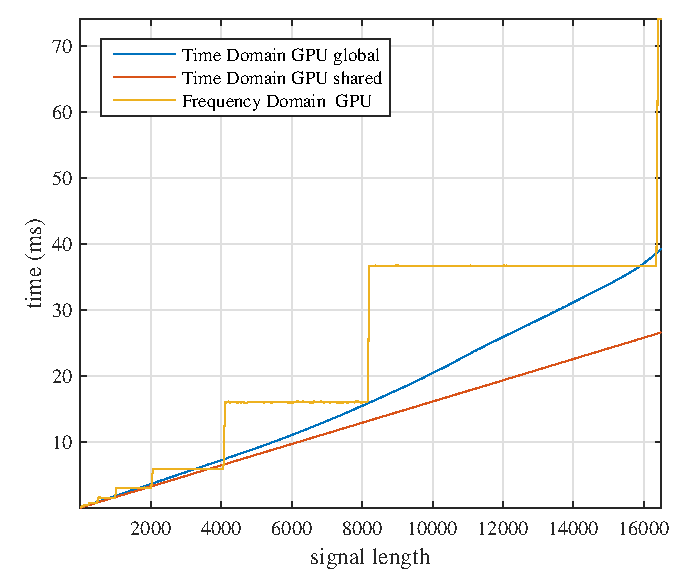
\includegraphics[width=5in]{figures/gpu_intro/CPUvsGPU_3104batch_21taps_varySignal.eps}
	\label{fig:CPUvsGPU_3104batch_21taps_varySignal}
\end{figure}

Figure \ref{fig:CPUvsGPU_3104batch_12672signal_varyFilter} shows execution time for $3104$ batches of $12672$ sample signal convolved with varying filter lengths.
This figure exhibits nearly the same characteristics of single batch convolution execution time shown in Figure \ref{fig:CPUvsGPU_1batch_12672signal_varyFilter} accept the varied filter length has no affect on execution time.
For very short filter lengths, time domain convolution using shared memory is fastest.
For longer filters , frequency domain convolution is fastest.
\begin{figure}
	\caption{Comparison of a batched complex convolution on a GPU. The signal length is varied and the filter is fixed at $21$ taps.}
	\centering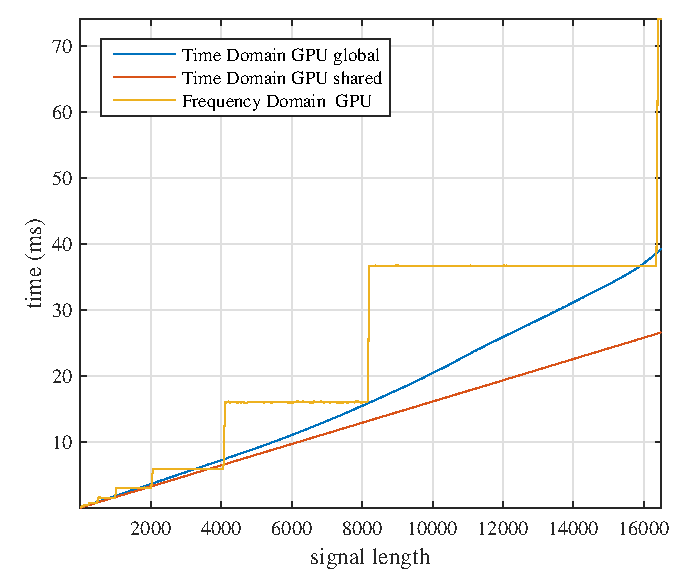
\includegraphics[width=5in]{figures/gpu_intro/CPUvsGPU_3104batch_21taps_varySignal.eps}
	\label{fig:CPUvsGPU_3104batch_21taps_varySignal}
\end{figure}

Though this section has show that in batched processing the algorithm leading to the fastest execution time still depends on signal and filter length,
one important comcept has been over looked.
Figure \ref{fig:ProcessingBlock} shows there are two filters that need to be allied to the signal. 

If convolution is implemented in the time domain, ConvGPU or ConvGPUshared must run twice.
The first call of ConvGPU or ConvGPUshared performs the convolution of the $186$ tap equalizer and $21$ detection filter.
The second call of ConvGPU or ConvGPUshared performs the convolution of the $12672$ sample signal with the  convolved $186+21-1$ tap filter.

If convolution is implemented in the frequency domain, only the GPU kernel PointToPointMultiply has to be updated.
PointToPointMultiply must be changed from two input vectors to three input vectors.
For every point the number of memory accesses increases by $1$ element and the number of flops doubles from $6$ to $12$.
An extra cuFFT call would be expected accept the detection filter in Figure \ref{fig:ProcessingBlock} constant.
The FFT of the detection filter can be calculated and stored at initialization.

Table \ref{tab:Batched_CPUvsGPUtable_12672_186} shows the batched convolution execution time for a $12672$ sample signal and $186$ tap filter.
Table \ref{tab:Batched_CPUvsGPUtable_12672_21} shows the batched convolution execution time for a $12672$ sample signal and $21$ tap filter.
Table \ref{tab:Batched_CPUvsGPUtable_12672_21_186} shows the batched cascaded convolution execution time for a $12672$ sample signal with $21$ and $186$ tap filters.
\begin{table}
\caption{Batched convolution execution times with for a $12672$ sample signal and $186$ tap filter on a Tesla K40c GPU.}
\begin{center}
\begin{tabular}{lll}
	\toprule
	Algorithm 				& Function or Library		& Execution Time (ms) \\ \midrule
	GPU time domain global 	& ConvGPU 					& 201.29		\\
	GPU time domain shared 	& ConvGPUshared 			& 180.272		\\
	GPU frequency domain 	& cuFFT						& 36.798 		\\ 
	\bottomrule
\end{tabular}
\end{center}
\label{tab:Batched_CPUvsGPUtable_12672_186}
\end{table}
\begin{table}
\caption{Batched convolution execution times with for a $12672$ sample signal and $21$ tap filter on a Tesla K40c GPU.}
\begin{center}
\begin{tabular}{lll}
	\toprule
	Algorithm 				& Function or Library		& Execution Time (ms) \\ \midrule
	GPU time domain global 	& ConvGPU 					& 27.642		\\
	GPU time domain shared 	& ConvGPUshared 			& 20.4287		\\
	GPU frequency domain 	& cuFFT						& 36.7604		\\ 
	\bottomrule
\end{tabular}
\end{center}
\label{tab:Batched_CPUvsGPUtable_12672_21}
\end{table}
\begin{table}
\caption{Batched convolution execution times with for a $12672$ sample signal and $206$ tap filter on a Tesla K40c GPU.}
\begin{center}
\begin{tabular}{lll}
	\toprule
	Algorithm 				& Function or Library		& Execution Time (ms) \\ \midrule
	GPU time domain global 	& ConvGPU 					& 223.064		\\
	GPU time domain shared 	& ConvGPUshared 			& 199.844		\\
	GPU frequency domain 	& cuFFT						& 36.7704		\\ 
	\bottomrule
\end{tabular}
\end{center}
\label{tab:Batched_CPUvsGPUtable_12672_206}
\end{table}
\begin{table}
\caption{Batched convolution execution times with for a $12672$ sample signal and cascaded $21$ and $186$ tap filter on a Tesla K40c GPU.}
\begin{center}
\begin{tabular}{lll}
	\toprule
	Algorithm 				& Function or Library		& Execution Time (ms) \\ \midrule
	GPU time domain global 	& ConvGPU 					& 223.307		\\
	GPU time domain shared 	& ConvGPUshared 			& 200.018		\\
	GPU frequency domain 	& cuFFT						& 39.0769		\\ 
	\bottomrule
\end{tabular}
\end{center}
\label{tab:Batched_CPUvsGPUtable_12672_21_186}
\end{table}

Tables \ref{tab:Batched_CPUvsGPUtable_12672_186} and \ref{tab:Batched_CPUvsGPUtable_12672_21} agree with Figures \ref{fig:CPUvsGPU_3104batch_21taps_varySignal} and \ref{fig:CPUvsGPU_3104batch_186taps_varySignal}.
Time domain convolution is faster with a short $21$ tap filter but frequency domain convolution is faster with a long $186$ tap filter.

\begin{figure}
	\caption{Two ways to convolve the signal $\mathbf{r}$ with the $186$ tap filter $\mathbf{c}$ and $21$ tap filter $\mathbf{d}$.}
	\centering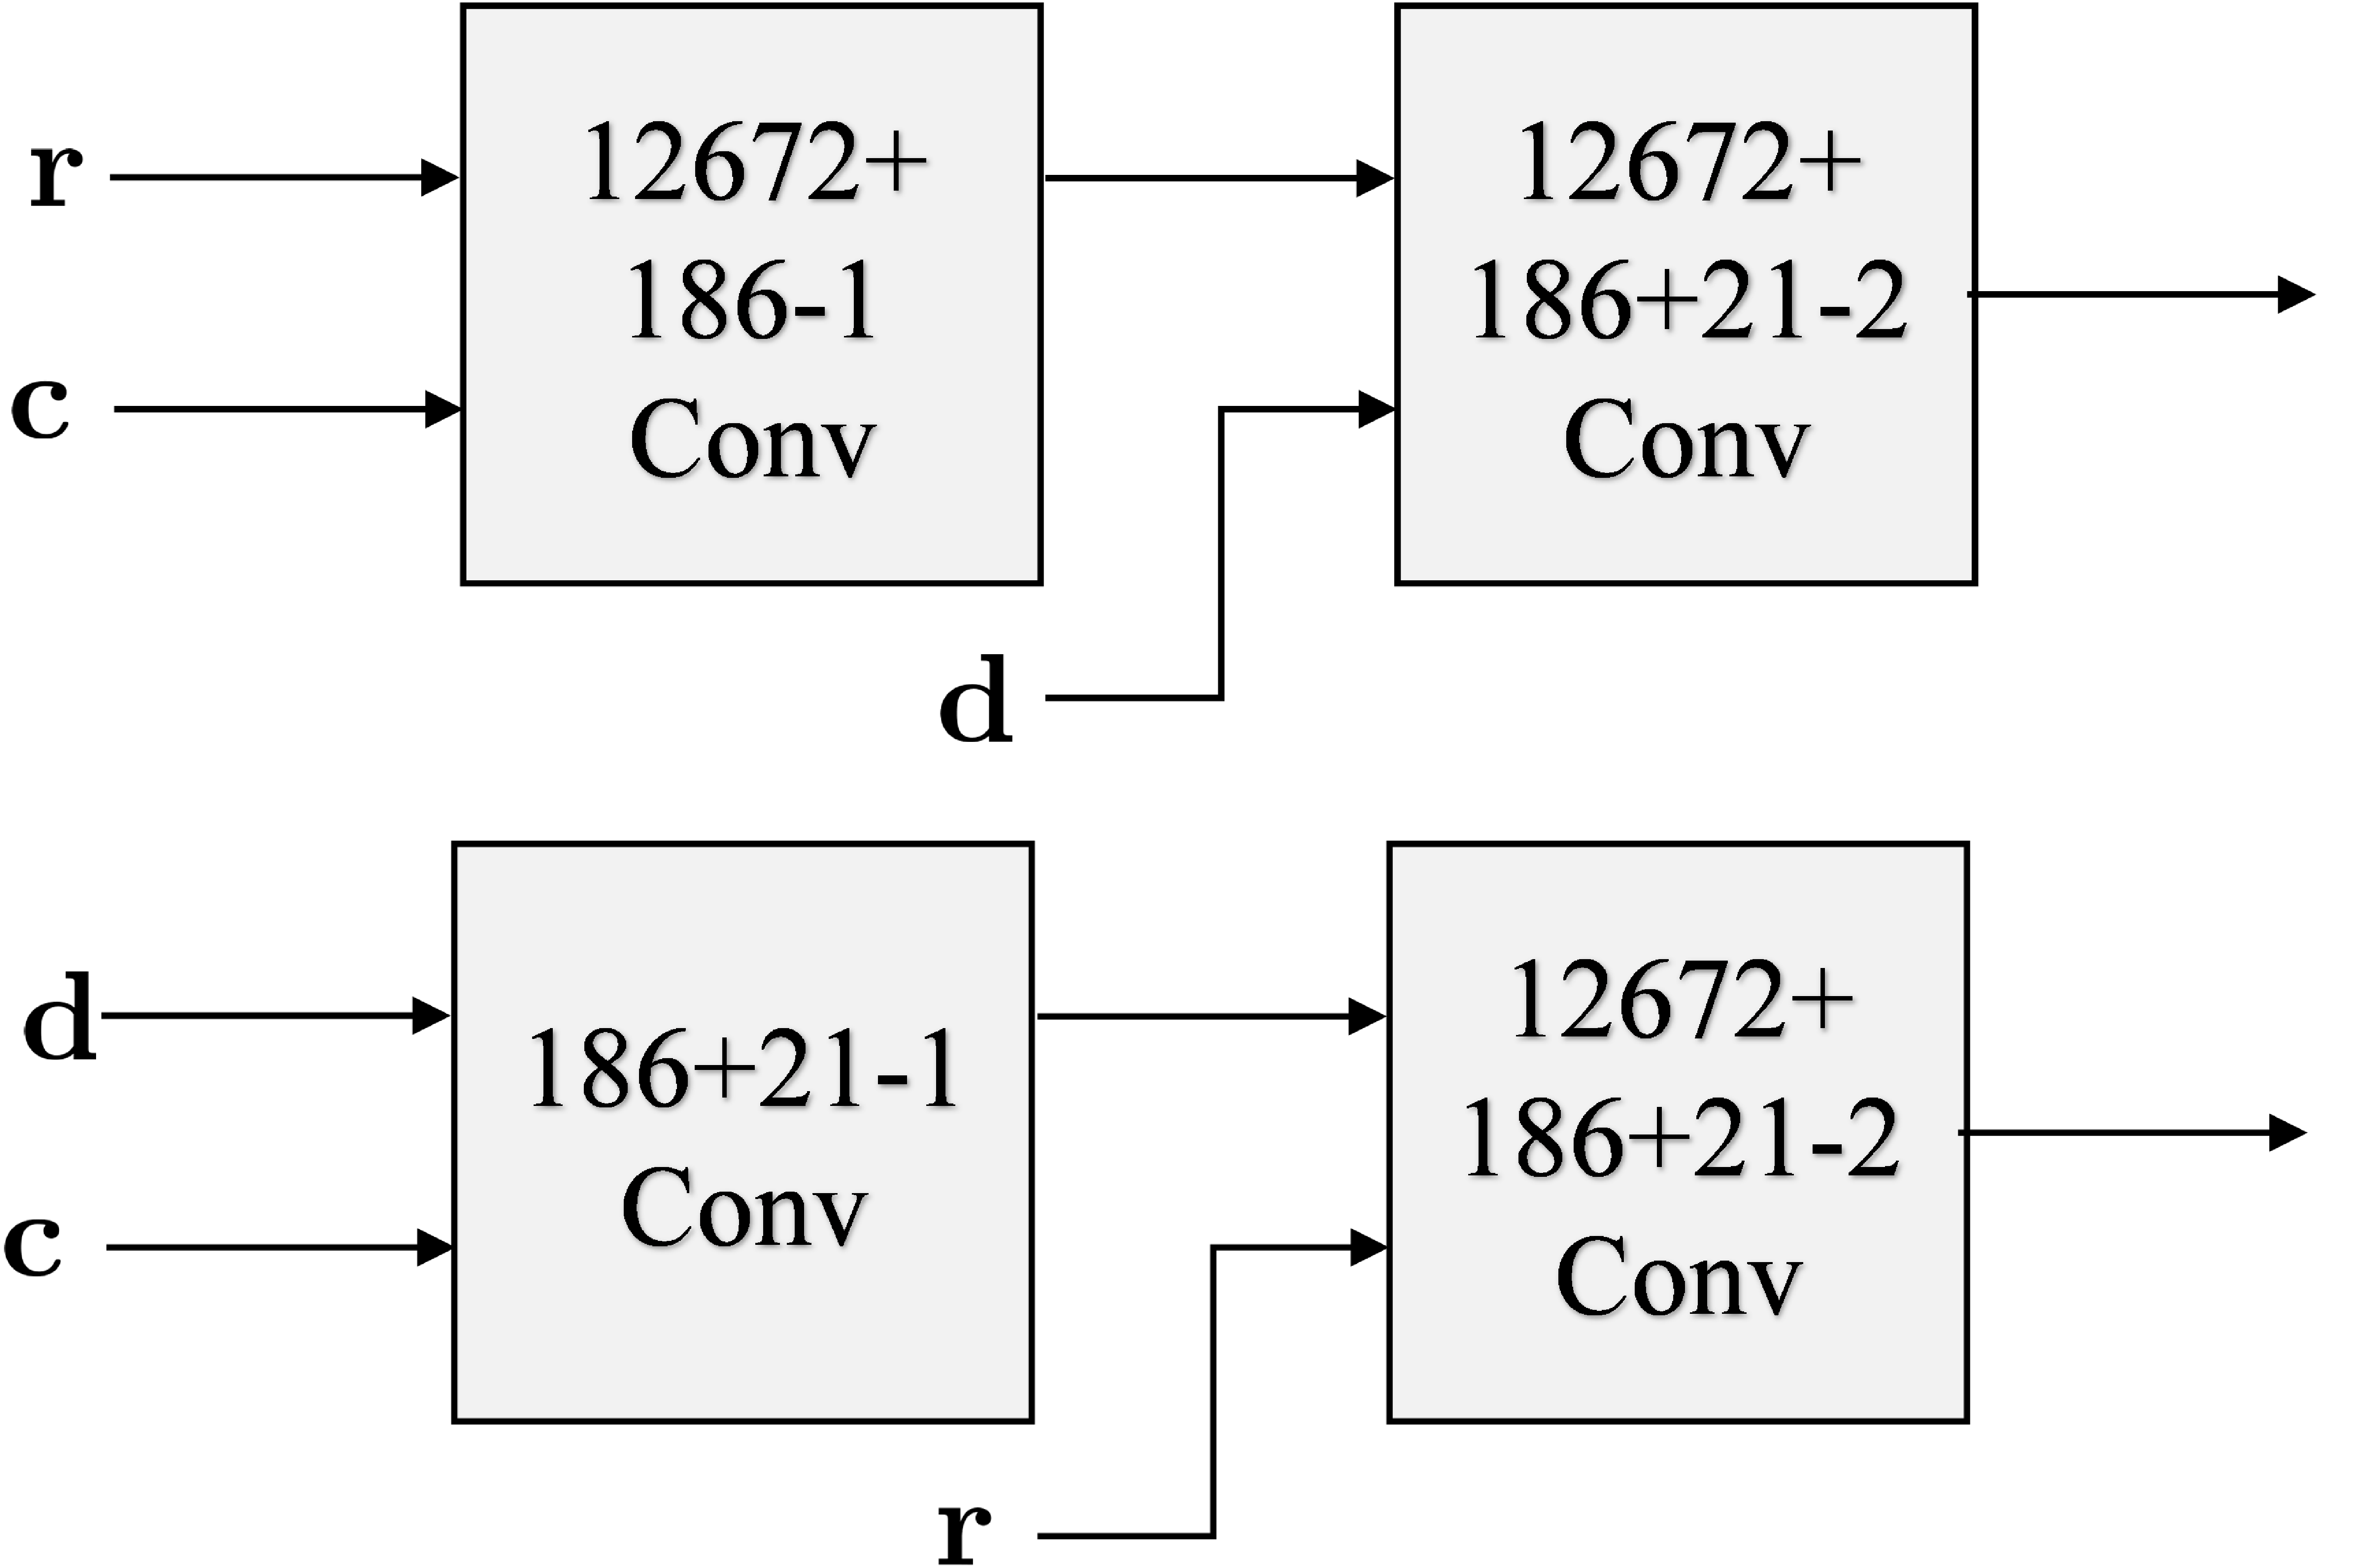
\includegraphics[width=5.01in/100*55]{figures/gpu_intro/twoWaysToConv.pdf}
	\label{fig:twoWaysToConv}
\end{figure}
Figure \ref{fig:twoWaysToConv} shows two ways to cascade the signal $\mathbf{r}$ though two filters.
Rather than applying both filters to the signal, compute a shorter convolution of the $186$ and $21$ tap filters then apply the $186+21-1$ tap result to the signal.

Table \ref{tab:Batched_CPUvsGPUtable_12672_21_186} shows the execution time of implementing cascaded filters, convolving the $21$ and $186$ tap filters is extremely fast in the GPU.
It only costs $2.3165$ms to apply an extra filter in the frequency domain.
It costs $22.0170$ms and $19.7460$ms to apply an extra filter in the time domain because the cascaded filter is now $206$ taps rather than $186$.
Table \ref{tab:Batched_CPUvsGPUtable_12672_206} confirms it costs an extra $20$ms or so to apply a $206$ vs $186$ tap filter.

Figure \ref{fig:CPUvsGPU_3104batch_21taps_186taps_cascade_varySignal} shows 
\begin{figure}
	\caption{Comparison of a batched cascaded complex convolution on a GPU. The signal length is varied and the filter is the $206$ result of convolving $186$ and $21$ tap filters.}
	\centering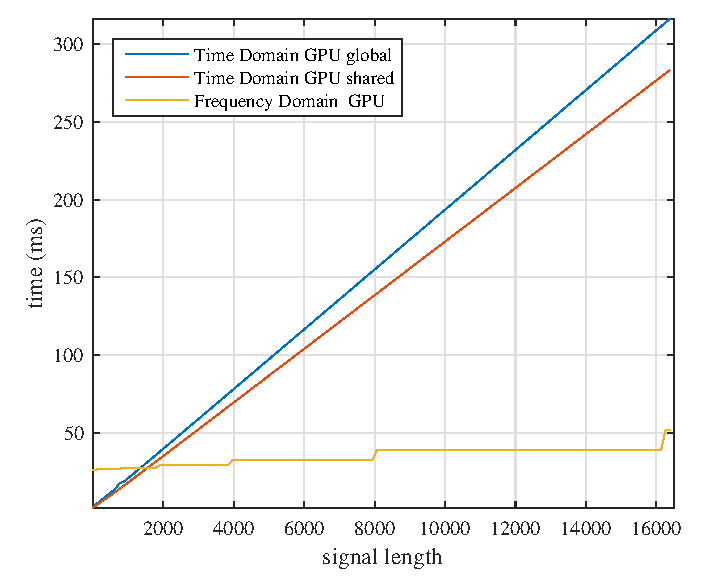
\includegraphics[width=5in]{figures/gpu_intro/CPUvsGPU_3104batch_21taps_186taps_cascade_varySignal.eps}
	\label{fig:CPUvsGPU_3104batch_21taps_186taps_cascade_varySignal}
\end{figure}


\singlespacing
\clearpage
\begin{lstlisting}[style=myCUDAstyle,language=C++,caption={CUDA code to performing complex convolution five different ways: time domain CPU, frequency domain CPU time domain GPU, time domain GPU using shared memory and frequency domain GPU.},label={code:convFun}]
#include <iostream>
#include <stdlib.h>
#include <math.h>
#include <cufft.h>
#include <fstream>
#include <string>
#include <fftw3.h>
using namespace std;


void ConvCPU(cufftComplex* y,cufftComplex* x,cufftComplex* h,int Lx,int Lh){
	for(int yIdx = 0; yIdx < Lx+Lh-1; yIdx++){
		cufftComplex temp;
		temp.x = 0;
		temp.y = 0;
		for(int hIdx = 0; hIdx < Lh; hIdx++){
			int xAccessIdx = yIdx-hIdx;
			if(xAccessIdx>=0 && xAccessIdx<Lx){
				// temp += x[xAccessIdx]*h[hIdx];
				float A = x[xAccessIdx].x;
				float B = x[xAccessIdx].y;
				float C = h[hIdx].x;
				float D = h[hIdx].y;
				cufftComplex result;
				result.x = A*C-B*D;
				result.y = A*D+B*C;
				temp.x += result.x;
				temp.y += result.y;
			}
		}
		y[yIdx] = temp;
	}

}

__global__ void ConvGPU(cufftComplex* y,cufftComplex* x,cufftComplex* h,int Lx,int Lh){
	int yIdx = blockIdx.x*blockDim.x + threadIdx.x;

	int lastThread = Lx+Lh-1;

	// don't access elements out of bounds
	if(yIdx >= lastThread)
		return;

	cufftComplex temp;
	temp.x = 0;
	temp.y = 0;
	for(int hIdx = 0; hIdx < Lh; hIdx++){
		int xAccessIdx = yIdx-hIdx;
		if(xAccessIdx>=0 && xAccessIdx<Lx){
			// temp += x[xAccessIdx]*h[hIdx];
			float A = x[xAccessIdx].x;
			float B = x[xAccessIdx].y;
			float C = h[hIdx].x;
			float D = h[hIdx].y;
			cufftComplex result;
			result.x = A*C-B*D;
			result.y = A*D+B*C;
			temp.x += result.x;
			temp.y += result.y;
		}
	}
	y[yIdx] = temp;
}


__global__ void ConvGPUshared(cufftComplex* y,cufftComplex* x,cufftComplex* h,int Lx,int Lh){
	int yIdx = blockIdx.x*blockDim.x + threadIdx.x;

	int lastThread = Lx+Lh-1;

	extern __shared__ cufftComplex h_shared[];
	if(threadIdx.x < Lh){
		h_shared[threadIdx.x] = h[threadIdx.x];
	}
	__syncthreads();

	// don't access elements out of bounds
	if(yIdx >= lastThread)
		return;

	cufftComplex temp;
	temp.x = 0;
	temp.y = 0;
	for(int hIdx = 0; hIdx < Lh; hIdx++){
		int xAccessIdx = yIdx-hIdx;
		if(xAccessIdx>=0 && xAccessIdx<Lx){
			// temp += x[xAccessIdx]*h[hIdx];
			float A = x[xAccessIdx].x;
			float B = x[xAccessIdx].y;
			float C = h_shared[hIdx].x;
			float D = h_shared[hIdx].y;
			cufftComplex result;
			result.x = A*C-B*D;
			result.y = A*D+B*C;
			temp.x += result.x;
			temp.y += result.y;
		}
	}
	y[yIdx] = temp;
}

__global__ void PointToPointMultiply(cufftComplex* v0, cufftComplex* v1, int lastThread){
	int i = blockIdx.x*blockDim.x + threadIdx.x;

	// don't access elements out of bounds
	if(i >= lastThread)
		return;
	float A = v0[i].x;
	float B = v0[i].y;
	float C = v1[i].x;
	float D = v1[i].y;

	// (A+jB)(C+jD) = (AC-BD) + j(AD+BC)
	cufftComplex result;
	result.x = A*C-B*D;
	result.y = A*D+B*C;

	v0[i] = result;
}

__global__ void ScalarMultiply(cufftComplex* vec0, float scalar, int lastThread){
	int i = blockIdx.x*blockDim.x + threadIdx.x;

	// Don't access elements out of bounds
	if(i >= lastThread)
		return;
	cufftComplex scalarMult;
	scalarMult.x = vec0[i].x*scalar;
	scalarMult.y = vec0[i].y*scalar;
	vec0[i] = scalarMult;
}

int main(){
	int mySignalLength = 1000;
	int myFilterLength = 186;
	int myConvLength   = mySignalLength + myFilterLength - 1;
	int Nfft           = pow(2, ceil(log(myConvLength)/log(2)));

	cufftComplex *mySignal1;
	cufftComplex *mySignal2;
	cufftComplex *mySignal2_fft;

	cufftComplex *myFilter1;
	cufftComplex *myFilter2;
	cufftComplex *myFilter2_fft;

	cufftComplex *myConv1;
	cufftComplex *myConv2;
	cufftComplex *myConv2_timeReversed;
	cufftComplex *myConv3;
	cufftComplex *myConv4;
	cufftComplex *myConv5;

	mySignal1      		= (cufftComplex*)malloc(mySignalLength*sizeof(cufftComplex));
	mySignal2      		= (cufftComplex*)malloc(Nfft  		  *sizeof(cufftComplex));
	mySignal2_fft  		= (cufftComplex*)malloc(Nfft   	      *sizeof(cufftComplex));

	myFilter1      		= (cufftComplex*)malloc(myFilterLength*sizeof(cufftComplex));
	myFilter2      		= (cufftComplex*)malloc(Nfft   	      *sizeof(cufftComplex));
	myFilter2_fft  		= (cufftComplex*)malloc(Nfft  		  *sizeof(cufftComplex));

	myConv1        		= (cufftComplex*)malloc(myConvLength  *sizeof(cufftComplex));
	myConv2        		= (cufftComplex*)malloc(Nfft  	      *sizeof(cufftComplex));
	myConv2_timeReversed= (cufftComplex*)malloc(Nfft  	      *sizeof(cufftComplex));
	myConv3        		= (cufftComplex*)malloc(myConvLength  *sizeof(cufftComplex));
	myConv4        		= (cufftComplex*)malloc(myConvLength  *sizeof(cufftComplex));
	myConv5        		= (cufftComplex*)malloc(Nfft          *sizeof(cufftComplex));

	srand(time(0));
	for(int i = 0; i < mySignalLength; i++){
		mySignal1[i].x = rand()%100-50;
		mySignal1[i].y = rand()%100-50;
	}

	for(int i = 0; i < myFilterLength; i++){
		myFilter1[i].x = rand()%100-50;
		myFilter1[i].y = rand()%100-50;
	}

	cufftComplex *dev_mySignal3;
	cufftComplex *dev_mySignal4;
	cufftComplex *dev_mySignal5;

	cufftComplex *dev_myFilter3;
	cufftComplex *dev_myFilter4;
	cufftComplex *dev_myFilter5;

	cufftComplex *dev_myConv3;
	cufftComplex *dev_myConv4;
	cufftComplex *dev_myConv5;

	cudaMalloc(&dev_mySignal3, mySignalLength*sizeof(cufftComplex));
	cudaMalloc(&dev_mySignal4, mySignalLength*sizeof(cufftComplex));
	cudaMalloc(&dev_mySignal5, Nfft          *sizeof(cufftComplex));

	cudaMalloc(&dev_myFilter3, myFilterLength*sizeof(cufftComplex));
	cudaMalloc(&dev_myFilter4, myFilterLength*sizeof(cufftComplex));
	cudaMalloc(&dev_myFilter5, Nfft          *sizeof(cufftComplex));

	cudaMalloc(&dev_myConv3,   myConvLength  *sizeof(cufftComplex));
	cudaMalloc(&dev_myConv4,   myConvLength  *sizeof(cufftComplex));
	cudaMalloc(&dev_myConv5,   Nfft          *sizeof(cufftComplex));


	/**
	 * Time Domain Convolution CPU
	 */
	ConvCPU(myConv1,mySignal1,myFilter1,mySignalLength,myFilterLength);

	/**
	 * Frequency Domain Convolution CPU
	 */
	fftwf_plan forwardPlanSignal = fftwf_plan_dft_1d(Nfft, (fftwf_complex*)mySignal2,    (fftwf_complex*)mySignal2_fft, 	   FFTW_FORWARD, FFTW_MEASURE);
	fftwf_plan forwardPlanFilter = fftwf_plan_dft_1d(Nfft, (fftwf_complex*)myFilter2, 	 (fftwf_complex*)myFilter2_fft, 	   FFTW_FORWARD, FFTW_MEASURE);
	fftwf_plan backwardPlanConv  = fftwf_plan_dft_1d(Nfft, (fftwf_complex*)mySignal2_fft,(fftwf_complex*)myConv2_timeReversed, FFTW_FORWARD, FFTW_MEASURE);

	cufftComplex zero; zero.x = 0; zero.y = 0;
	for(int i = 0; i < Nfft; i++){
		if(i<mySignalLength)
			mySignal2[i] = mySignal1[i];
		else
			mySignal2[i] = zero;

		if(i<myFilterLength)
			myFilter2[i] = myFilter1[i];
		else
			myFilter2[i] = zero;
	}

	fftwf_execute(forwardPlanSignal);
	fftwf_execute(forwardPlanFilter);

	for (int i = 0; i < Nfft; i++){
		// mySignal2_fft = mySignal2_fft*myFilter2_fft;
		float A = mySignal2_fft[i].x;
		float B = mySignal2_fft[i].y;
		float C = myFilter2_fft[i].x;
		float D = myFilter2_fft[i].y;
		cufftComplex result;
		result.x = A*C-B*D;
		result.y = A*D+B*C;
		mySignal2_fft[i] = result;
	}

	fftwf_execute(backwardPlanConv);

	// myConv2 from fftwf must be time reversed and scaled
	// to match Matlab, myConv1, myConv3, myConv4 and myConv5
	cufftComplex result;
	for (int i = 0; i < Nfft; i++){
		result.x = myConv2_timeReversed[Nfft-i].x/Nfft;
		result.y = myConv2_timeReversed[Nfft-i].y/Nfft;
		myConv2[i] = result;
	}
	result.x = myConv2_timeReversed[0].x/Nfft;
	result.y = myConv2_timeReversed[0].y/Nfft;
	myConv2[0] = result;

	fftwf_destroy_plan(forwardPlanSignal);
	fftwf_destroy_plan(forwardPlanFilter);
	fftwf_destroy_plan(backwardPlanConv);


	/**
	 * Time Domain Convolution GPU Using Global Memory
	 */
	cudaMemcpy(dev_mySignal3, mySignal1, sizeof(cufftComplex)*mySignalLength, cudaMemcpyHostToDevice);
	cudaMemcpy(dev_myFilter3, myFilter1, sizeof(cufftComplex)*myFilterLength, cudaMemcpyHostToDevice);

	int numTreadsPerBlock = 512;
	int numBlocks = myConvLength/numTreadsPerBlock;
	if(myConvLength % numTreadsPerBlock > 0)
		numBlocks++;
	ConvGPU<<<numBlocks, numTreadsPerBlock>>>(dev_myConv3, dev_mySignal3, dev_myFilter3, mySignalLength, myFilterLength);

	cudaMemcpy(myConv3, dev_myConv3, myConvLength*sizeof(cufftComplex), cudaMemcpyDeviceToHost);


	/**
	 * Time Domain Convolution GPU Using Shared Memory
	 */
	cudaMemcpy(dev_mySignal4, mySignal1, sizeof(cufftComplex)*mySignalLength, cudaMemcpyHostToDevice);
	cudaMemcpy(dev_myFilter4, myFilter1, sizeof(cufftComplex)*myFilterLength, cudaMemcpyHostToDevice);

	numTreadsPerBlock = 512;
	numBlocks = myConvLength/numTreadsPerBlock;
	if(myConvLength % numTreadsPerBlock > 0)
		numBlocks++;
	ConvGPUshared<<<numBlocks, numTreadsPerBlock,myFilterLength*sizeof(cufftComplex)>>>(dev_myConv4, dev_mySignal4, dev_myFilter4, mySignalLength, myFilterLength);

	cudaMemcpy(myConv4, dev_myConv4, myConvLength*sizeof(cufftComplex), cudaMemcpyDeviceToHost);


	/**
	 * Frequency Domain Convolution GPU
	 */
	cufftHandle plan;
	int n[1] = {Nfft};
	cufftPlanMany(&plan,1,n,NULL,1,1,NULL,1,1,CUFFT_C2C,1);

	cudaMemset(dev_mySignal5, 0, 	     Nfft*sizeof(cufftComplex));
	cudaMemset(dev_myFilter5, 0, 	     Nfft*sizeof(cufftComplex));

	cudaMemcpy(dev_mySignal5, mySignal2, Nfft*sizeof(cufftComplex), cudaMemcpyHostToDevice);
	cudaMemcpy(dev_myFilter5, myFilter2, Nfft*sizeof(cufftComplex), cudaMemcpyHostToDevice);

	cufftExecC2C(plan, dev_mySignal5, dev_mySignal5, CUFFT_FORWARD);
	cufftExecC2C(plan, dev_myFilter5, dev_myFilter5, CUFFT_FORWARD);

	numTreadsPerBlock = 512;
	numBlocks = Nfft/numTreadsPerBlock;
	if(Nfft % numTreadsPerBlock > 0)
		numBlocks++;
	PointToPointMultiply<<<numBlocks, numTreadsPerBlock>>>(dev_mySignal5, dev_myFilter5, Nfft);

	cufftExecC2C(plan, dev_mySignal5, dev_mySignal5, CUFFT_INVERSE);

	numTreadsPerBlock = 128;
	numBlocks = Nfft/numTreadsPerBlock;
	if(Nfft % numTreadsPerBlock > 0)
		numBlocks++;
	float scalar = 1.0/((float)Nfft);
	ScalarMultiply<<<numBlocks, numTreadsPerBlock>>>(dev_mySignal5, scalar, Nfft);

	cudaMemcpy(myConv5, dev_mySignal5, Nfft*sizeof(cufftComplex), cudaMemcpyDeviceToHost);

	cufftDestroy(plan);

	free(mySignal1);
	free(mySignal2);

	free(myFilter1);
	free(myFilter2);

	free(myConv1);
	free(myConv2);
	free(myConv2_timeReversed);
	free(myConv3);
	free(myConv4);
	free(myConv5);
	fftwf_cleanup();

	cudaFree(dev_mySignal3);
	cudaFree(dev_mySignal4);
	cudaFree(dev_mySignal5);

	cudaFree(dev_myFilter3);
	cudaFree(dev_myFilter4);
	cudaFree(dev_myFilter5);

	cudaFree(dev_myConv3);
	cudaFree(dev_myConv4);
	cudaFree(dev_myConv5);

	return 0;
}
\end{lstlisting}
\doublespacing

\singlespacing
\clearpage
\begin{lstlisting}[style=myCUDAstyle,language=C++,caption={CUDA code to perform batched complex convolution three different ways in a GPU: time domain using global memory, time domain using shared memory and frequency domain GPU.},label={code:batchedConvFun}]
#include <cufft.h>
#include <iostream>
using namespace std;

__global__ void ConvGPU(cufftComplex* y_out,cufftComplex* x_in,cufftComplex* h_in,int Lx,int Lh,int maxThreads){
	int threadNum = blockIdx.x*blockDim.x + threadIdx.x;
	int convLength = Lx+Lh-1;

	// Don't access elements out of bounds
	if(threadNum >= maxThreads)
		return;

	int batch = threadNum/convLength;
	int yIdx  = threadNum%convLength;
	cufftComplex* x = &x_in[Lx*batch];
	cufftComplex* h = &h_in[Lh*batch];
	cufftComplex* y = &y_out[convLength*batch];

	cufftComplex temp;
	temp.x = 0;
	temp.y = 0;
	for(int hIdx = 0; hIdx < Lh; hIdx++){
		int xAccessIdx = yIdx-hIdx;
		if(xAccessIdx>=0 && xAccessIdx<Lx){
			// temp += x[xAccessIdx]*h[hIdx];
			// (A+jB)(C+jD) = (AC-BD) + j(AD+BC)
			float A = x[xAccessIdx].x;
			float B = x[xAccessIdx].y;
			float C = h[hIdx].x;
			float D = h[hIdx].y;
			cufftComplex complexMult;
			complexMult.x = A*C-B*D;
			complexMult.y = A*D+B*C;

			temp.x += complexMult.x;
			temp.y += complexMult.y;
		}
	}
	y[yIdx] = temp;
}

__global__ void ConvGPUshared(cufftComplex* y_out,cufftComplex* x_in,cufftComplex* h_in,int Lx,int Lh,int maxThreads){

	int threadNum = blockIdx.x*blockDim.x + threadIdx.x;
	int convLength = Lx+Lh-1;
	// Don't access elements out of bounds
	if(threadNum >= maxThreads)
		return;

	int batch = threadNum/convLength;
	int yIdx  = threadNum%convLength;
	cufftComplex* x = &x_in[Lx*batch];
	cufftComplex* h = &h_in[Lh*batch];
	cufftComplex* y = &y_out[convLength*batch];

	extern __shared__ cufftComplex h_shared[];
	if(threadIdx.x < Lh)
		h_shared[threadIdx.x] = h[threadIdx.x];

	__syncthreads();

	cufftComplex temp;
	temp.x = 0;
	temp.y = 0;
	for(int hIdx = 0; hIdx < Lh; hIdx++){
		int xAccessIdx = yIdx-hIdx;
		if(xAccessIdx>=0 && xAccessIdx<Lx){
			// temp += x[xAccessIdx]*h[hIdx];
			// (A+jB)(C+jD) = (AC-BD) + j(AD+BC)
			float A = x[xAccessIdx].x;
			float B = x[xAccessIdx].y;
			float C = h_shared[hIdx].x;
			float D = h_shared[hIdx].y;
			cufftComplex complexMult;
			complexMult.x = A*C-B*D;
			complexMult.y = A*D+B*C;

			temp.x += complexMult.x;
			temp.y += complexMult.y;
		}
	}
	y[yIdx] = temp;
}

__global__ void PointToPointMultiply(cufftComplex* vec0, cufftComplex* vec1, int maxThreads){
	int i = blockIdx.x*blockDim.x + threadIdx.x;
	// Don't access elements out of bounds
	if(i >= maxThreads)
		return;
	// vec0[i] = vec0[i]*vec1[i];
	// (A+jB)(C+jD) = (AC-BD) + j(AD+BC)
	float A = vec0[i].x;
	float B = vec0[i].y;
	float C = vec1[i].x;
	float D = vec1[i].y;
	cufftComplex complexMult;
	complexMult.x = A*C-B*D;
	complexMult.y = A*D+B*C;
	vec0[i] = complexMult;
}

__global__ void ScalarMultiply(cufftComplex* vec0, float scalar, int lastThread){
	int i = blockIdx.x*blockDim.x + threadIdx.x;
	// Don't access elements out of bounds
	if(i >= lastThread)
		return;
	cufftComplex scalarMult;
	scalarMult.x = vec0[i].x*scalar;
	scalarMult.y = vec0[i].y*scalar;
	vec0[i] = scalarMult;
}

int main(){
	int numBatches     = 3104;
	int mySignalLength = 12672;
	int myFilterLength = 186;
	int myConvLength   = mySignalLength + myFilterLength - 1;
	int Nfft           = pow(2, ceil(log(myConvLength)/log(2)));
	int maxThreads;
	int numTreadsPerBlock;
	int numBlocks;

	cufftHandle plan;
	int n[1] = {Nfft};
	cufftPlanMany(&plan,1,n,NULL,1,1,NULL,1,1,CUFFT_C2C,numBatches);

	// Allocate memory on host
	cufftComplex *mySignal1;
	cufftComplex *mySignal1_pad;
	cufftComplex *myFilter1;
	cufftComplex *myFilter1_pad;
	cufftComplex *myConv1;
	cufftComplex *myConv2;
	cufftComplex *myConv3;
	mySignal1      = (cufftComplex*) malloc(mySignalLength*numBatches*sizeof(cufftComplex));
	mySignal1_pad  = (cufftComplex*) malloc(Nfft		  *numBatches*sizeof(cufftComplex));
	myFilter1      = (cufftComplex*) malloc(myFilterLength*numBatches*sizeof(cufftComplex));
	myFilter1_pad  = (cufftComplex*) malloc(Nfft	      *numBatches*sizeof(cufftComplex));
	myConv1        = (cufftComplex*) malloc(myConvLength  *numBatches*sizeof(cufftComplex));
	myConv2        = (cufftComplex*) malloc(myConvLength  *numBatches*sizeof(cufftComplex));
	myConv3        = (cufftComplex*) malloc(Nfft		  *numBatches*sizeof(cufftComplex));

	srand(time(0));
	for(int i = 0; i < mySignalLength; i++){
		mySignal1[i].x = rand()%100-50;
		mySignal1[i].y = rand()%100-50;
	}

	for(int i = 0; i < myFilterLength; i++){
		myFilter1[i].x = rand()%100-50;
		myFilter1[i].y = rand()%100-50;
	}

	cufftComplex zero;
	zero.x = 0;
	zero.y = 0;
	for(int i = 0; i<Nfft*numBatches; i++){
		mySignal1_pad[i] = zero;
		myFilter1_pad[i] = zero;
	}
	for(int batch=0; batch < numBatches; batch++){
		for(int i = 0; i < mySignalLength; i++){
			mySignal1[batch*mySignalLength+i] = mySignal1[i];
			mySignal1_pad[batch*Nfft+i] = mySignal1[i];
		}
		for(int i = 0; i < myFilterLength; i++){
			myFilter1[batch*myFilterLength+i] = myFilter1[i];
			myFilter1_pad[batch*Nfft+i] = myFilter1[i];
		}
	}

	// Allocate memory on device
	cufftComplex *dev_mySignal1;
	cufftComplex *dev_mySignal2;
	cufftComplex *dev_mySignal3;
	cufftComplex *dev_myFilter1;
	cufftComplex *dev_myFilter2;
	cufftComplex *dev_myFilter3;
	cufftComplex *dev_myConv1;
	cufftComplex *dev_myConv2;
	cufftComplex *dev_myConv3;
	cudaMalloc(&dev_mySignal1, mySignalLength*numBatches*sizeof(cufftComplex));
	cudaMalloc(&dev_mySignal2, mySignalLength*numBatches*sizeof(cufftComplex));
	cudaMalloc(&dev_mySignal3, Nfft		     *numBatches*sizeof(cufftComplex));
	cudaMalloc(&dev_myFilter1, myFilterLength*numBatches*sizeof(cufftComplex));
	cudaMalloc(&dev_myFilter2, myFilterLength*numBatches*sizeof(cufftComplex));
	cudaMalloc(&dev_myFilter3, Nfft			 *numBatches*sizeof(cufftComplex));
	cudaMalloc(&dev_myConv1,   myConvLength  *numBatches*sizeof(cufftComplex));
	cudaMalloc(&dev_myConv2,   myConvLength  *numBatches*sizeof(cufftComplex));
	cudaMalloc(&dev_myConv3,   Nfft  		 *numBatches*sizeof(cufftComplex));

	/**
	 * Time Domain Convolution GPU Using Global Memory
	 */
	cudaMemcpy(dev_mySignal1, mySignal1, numBatches*sizeof(cufftComplex)*mySignalLength, cudaMemcpyHostToDevice);
	cudaMemcpy(dev_myFilter1, myFilter1, numBatches*sizeof(cufftComplex)*myFilterLength, cudaMemcpyHostToDevice);

	maxThreads = myConvLength*numBatches;
	numTreadsPerBlock = 128;
	numBlocks = maxThreads/numTreadsPerBlock;
	if(maxThreads % numTreadsPerBlock > 0)
		numBlocks++;
	ConvGPU<<<numBlocks, numTreadsPerBlock>>>(dev_myConv1, dev_mySignal1, dev_myFilter1, mySignalLength, myFilterLength, maxThreads);

	cudaMemcpy(myConv1, dev_myConv1, myConvLength*numBatches*sizeof(cufftComplex), cudaMemcpyDeviceToHost);

	/**
	 * Time Domain Convolution GPU Using Shared Memory
	 */
	cudaMemcpy(dev_mySignal2, mySignal1, numBatches*sizeof(cufftComplex)*mySignalLength, cudaMemcpyHostToDevice);
	cudaMemcpy(dev_myFilter2, myFilter1, numBatches*sizeof(cufftComplex)*myFilterLength, cudaMemcpyHostToDevice);

	maxThreads = myConvLength*numBatches;
	numTreadsPerBlock = 256;
	numBlocks = maxThreads/numTreadsPerBlock;
	if(maxThreads % numTreadsPerBlock > 0)
		numBlocks++;
	ConvGPUshared<<<numBlocks, numTreadsPerBlock, myFilterLength*sizeof(cufftComplex)>>>(dev_myConv2, dev_mySignal2, dev_myFilter2, mySignalLength, myFilterLength,maxThreads);

	cudaMemcpy(myConv2, dev_myConv2, myConvLength*numBatches*sizeof(cufftComplex), cudaMemcpyDeviceToHost);

	/**
	 * Frequency Domain Convolution GPU
	 */
	cudaMemcpy(dev_mySignal3, mySignal1_pad, Nfft*numBatches*sizeof(cufftComplex), cudaMemcpyHostToDevice);
	cudaMemcpy(dev_myFilter3, myFilter1_pad, Nfft*numBatches*sizeof(cufftComplex), cudaMemcpyHostToDevice);

	cufftExecC2C(plan, dev_mySignal3, dev_mySignal3, CUFFT_FORWARD);
	cufftExecC2C(plan, dev_myFilter3, dev_myFilter3, CUFFT_FORWARD);

	maxThreads = Nfft*numBatches;
	numTreadsPerBlock = 96;
	numBlocks = maxThreads/numTreadsPerBlock;
	if(maxThreads % numTreadsPerBlock > 0)
		numBlocks++;
	PointToPointMultiply<<<numBlocks, numTreadsPerBlock>>>(dev_mySignal3, dev_myFilter3, maxThreads);
	cufftExecC2C(plan, dev_mySignal3, dev_mySignal3, CUFFT_INVERSE);

	numTreadsPerBlock = 640;
	numBlocks = maxThreads/numTreadsPerBlock;
	if(maxThreads % numTreadsPerBlock > 0)
		numBlocks++;
	float scalar = 1.0/((float)Nfft);
	ScalarMultiply<<<numBlocks, numTreadsPerBlock>>>(dev_mySignal3, scalar, maxThreads);

	cudaMemcpy(myConv3, dev_mySignal3, Nfft*numBatches*sizeof(cufftComplex), cudaMemcpyDeviceToHost);

	cufftDestroy(plan);

	// Free vectors on CPU
	free(mySignal1);
	free(myFilter1);
	free(myConv1);
	free(myConv2);
	free(myConv3);

	// Free vectors on GPU
	cudaFree(dev_mySignal1);
	cudaFree(dev_mySignal2);
	cudaFree(dev_mySignal3);
	cudaFree(dev_myFilter1);
	cudaFree(dev_myFilter2);
	cudaFree(dev_myFilter3);
	cudaFree(dev_myConv1);
	cudaFree(dev_myConv2);
	cudaFree(dev_myConv3);

	return 0;
}
\end{lstlisting}
\doublespacing
%%%%%%%%%%%%%%%%%%%%%%%%%%%%%%%%%%%%%%%%%%%%%%%%%%%%%%%%%%%%%%%%%%%%%%%%%%%%%%%%%%%%%%%%%%%%%%
%%%%%%%%%%%%%%%%%%%%%%%%%%%%%%%%%%%%%%%%%%%%%%%%%%%%%%%%%%%%%%%%%%%%%%%%%%%%%%%%%%%%%%%%%%%%%%
%%%%%%%%%%% GPU
%%%%%%%%%%%%%%%%%%%%%%%%%%%%%%%%%%%%%%%%%%%%%%%%%%%%%%%%%%%%%%%%%%%%%%%%%%%%%%%%%%%%%%%%%%%%%%
%%%%%%%%%%%%%%%%%%%%%%%%%%%%%%%%%%%%%%%%%%%%%%%%%%%%%%%%%%%%%%%%%%%%%%%%%%%%%%%%%%%%%%%%%%%%%%

% \cleardoublepage
\chapter{Equalizer Equations}
\label{chap:eq_eq}

\section{Overview}
This thesis examines that performance and GPU implementation of 5 equalizers.
While the performance and GPU implementation is interesting, this thesis makes no claim of theoretically expanding understanding of equalizers.
The data-aided equalizers studied in this thesis are:
\begin{itemize}
\item Zero-Forcing (ZF)
\item Minimum Mean Square Error (MMSE)
\item Constant Modulus Algorithm (CMA)
\item Frequency Domain Equalizer 1 (FDE1)
\item Frequency Domain Equalizer 2 (FDE2)
\end{itemize}

The ZF and MMSE equalizers are very similar in formulation though from different sources.
As you might tell from the names, FDE1 and FDE2 are very similar also with one subtle difference.
CMA isn't related to any other algorithm aside from being initialized to MMSE.

\section{Zero-Forcing and Minimum Mean Square Error Equalizers}

The ZF and MMSE equalizers are treated together here because they have many common features.
Both equalizers are found by solving linear equations
\begin{equation}
\mathbf{R}\mathbf{c} = \hat{\mathbf{h}}
\end{equation}
where $\mathbf{c}$ is vector of the desired equalizer coefficients
and $\mathbf{R}$ is the auto-correlation matrix of the channel estimate $\hat{\mathbf{h}}$.
It will be shown that the only difference between ZF and MMSE lies in the the auto-correlation matrix $\mathbf{R}$.

\subsection{Zero-Forcing}
The ZF equalizer is an FIR filter defined by the coefficients
\begin{equation}
\begin{matrix}
c_\text{ZF}(-L_1) & \cdots & c_\text{ZF}(0) & \cdots & c_\text{ZF}(L_2).
\end{matrix}
\end{equation}
The filter coefficients are the solution to the matrix vector equation \cite[eq. (311)]{PAQ-phase1}
\begin{equation}
\mathbf{c}_\text{ZF} = \big(\mathbf{H}^\dagger\mathbf{H}\big)^{-1} \mathbf{H}^\dagger \mathbf{u}_{n_0}
\label{eq:c_ZF_direct}
\end{equation}
where
\begin{equation}
\mathbf{c}_\text{ZF} = 
\begin{bmatrix}
c_\text{ZF}(-L_1) \\ \vdots \\ c_\text{ZF}(0) \\ \vdots \\ c_\text{ZF}(L_2)
\end{bmatrix},
\end{equation}
\begin{equation}
\mathbf{u}_{n_0} = \begin{bmatrix} 0 \\ \vdots \\ 0 \\ 1 \\ 0 \\ \vdots \\ 0 \end{bmatrix}
	\begin{matrix*}[l] \left. \vphantom{\begin{matrix} 0 \\ \vdots \\ 0 \end{matrix}} \right\}
		\text{$n_0-1$ zeros}
		\\ \\
		\left. \vphantom{\begin{matrix} 0 \\ \vdots \\ 0 \end{matrix}} \right\}
		\text{$N_1+N_2+L_1+L_2-n_0+1$ zeros}
		\end{matrix*},
		\label{eq:un0_ZF}
\end{equation}
and
\begin{equation} 
\mathbf{H} = 
		\begin{bmatrix}
		\hat{h}(-N_1)		&  				& 		 	&  					\\
		\hat{h}(-N_1+1) 	& \hat{h}(-N_1)	& 		 	&  					\\
		\vdots	 			& \vdots		& \ddots 	&  					\\
		\hat{h}(N_2)		& \hat{h}(N_2-1)&  			& \hat{h}(-N_1)  	\\
		 					& \hat{h}(N_2) 	&  			& \hat{h}(-N_1+1) 	\\
		 					&  	   			&  			& \vdots			\\
		 					&  	   			&  			& \hat{h}(N_2)		\\
	\end{bmatrix}.
\end{equation}

Calculating Equation \eqref{eq:c_ZF_direct} would give the desired result but the computation is heavy.
The heaviest computation is the $\mathcal{O}(n^3)$ inverse operation followed by the $\mathcal{O}(n^2)$ matrix matrix multiplies.
Rather than performing a heavy inverse, multiplying $\mathbf{H}^\dagger \mathbf{H}$ on both sides of equation \eqref{eq:c_ZF_direct} results in
\begin{align}
\mathbf{H}^\dagger\mathbf{H} \mathbf{c}_\text{ZF} &= \mathbf{H}^\dagger \mathbf{u}_{n_0} \nonumber \\
\mathbf{R}_{\hat{h}} \mathbf{c}_\text{ZF} &= \hat{\mathbf{h}}_{n_0}
\label{eq:c_ZF_solve}
\end{align}
where
\begin{equation}
\mathbf{R}_{\hat{h}} = 
\mathbf{H}^\dagger \mathbf{H} = 
		\begin{bmatrix}
		r_{\hat{h}}(0)			& r^\ast_{\hat{h}}(1)	& \cdots 	& r^\ast_{\hat{h}}(L_{eq}-1)  	\\
		r_{\hat{h}}(1) 			& r_{\hat{h}}(0)		& \cdots 	& r^\ast_{\hat{h}}(L_{eq}-2)  	\\
		\vdots	 				& \vdots				& \ddots 	&  								\\
		r_{\hat{h}}(L_{eq}-1)	& r_{\hat{h}}(L_{eq}-2)	& \cdots	& r_{\hat{h}}(0)  			
	\end{bmatrix}
	\label{eq:R_h}
\end{equation}
is the auto-correlation matrix of the channel estimate $\hat{\mathbf{h}}$ with 
\begin{equation}
r_{\hat{h}}(k) = \sum_{n=-N_1}^{N_2} \hat{h}(n) \hat{h}^\ast(n-k).
\end{equation}
and 
\begin{equation}
\hat{\mathbf{h}}_{n_0} = \mathbf{H}^\dagger \mathbf{u}_{n_0} = 
\begin{bmatrix} \hat{h}^\ast(L_1) \\ \vdots \\ \hat{h}^\ast(0) \\ \vdots \\ \hat{h}^\ast(-L_2)  \end{bmatrix}
\label{eq:h_no}
\end{equation}
is a vector with the time reversed and conjugated channel estimate $\hat{\mathbf{h}}$ centered at $n_0$.

Note that $\mathbf{R}_{\hat{h}}$ can be built by computing
\begin{equation}
\mathbf{r}_{\hat{h}} = 
\begin{bmatrix} r_{\hat{h}}(0) \\ \vdots \\ r_{\hat{h}}(L_{ch}) \\ r_{\hat{h}}(L_{ch}+1) \\ \vdots \\ r_{\hat{h}}(L_{eq}-1)\end{bmatrix} =
\begin{bmatrix} r_{\hat{h}}(0) \\ \vdots \\ r_{\hat{h}}(L_{ch}) \\ 0 \\ \vdots \\ 0  \end{bmatrix},
\end{equation} 
eliminating the need for matrix matrix multiply of $\mathbf{H}^\dagger\mathbf{H}$.
Also, $r_{\hat{h}}(k)$ only has support on $-L_{ch} \leq k \leq L_{ch}$ making $\mathbf{R}_{\hat{h}}$ sparse or $\%63$ zeros.
The sparseness of $\mathbf{R}_{\hat{h}}$ can be leveraged to reduce computation drastically.

%Jeff explains how CUDA solvers handle this equation.
%
%The ZF equalizer was studied in the PAQ Phase 1 Final Report in ~equation 324
%\begin{equation}
%\mathbf{c}_\text{ZF} = (\mathbf{H}^\dagger \mathbf{H})^{-1} \mathbf{H}^\dagger \mathbf{u}_{n_0}
%\label{eq:c_ZF_pinv}
%\end{equation}
%where $\mathbf{c}_\text{ZF}$ is a $L_{eq} \times 1$ vector of equalizer coefficients computed to invert the channel estimate $\hat{\mathbf{h}}$
%and $\mathbf{u}_{n_0}$ is the desired channel impulse response centered on $n0 = N_1+L_1+1$
%\begin{equation}
%\mathbf{u}_{n_0} = \begin{bmatrix} 0 \\ \vdots \\ 0 \\ 1 \\ 0 \\ \vdots \\ 0 \end{bmatrix}
%	\begin{matrix*}[l] \left. \vphantom{\begin{matrix} 0 \\ \vdots \\ 0 \end{matrix}} \right\}
%		\text{$n_0-1$ zeros}
%		\\ \\
%		\left. \vphantom{\begin{matrix} 0 \\ \vdots \\ 0 \end{matrix}} \right\}
%		\text{$N_1+N_2+L_1+L_2-n_0+1$ zeros}
%		\end{matrix*}.
%		\label{eq:un0_ZF}
%\end{equation}
%The $L_{eq}+N_1+N_2 \times L_{eq}$ convolution matrix $\mathbf{H}$ is built using the channel estimate $\hat{\mathbf{h}}$
%\begin{equation}
%\mathbf{H} = 
%		\begin{bmatrix}
%		h(-N_1)		&  			& 		 	&  			\\
%		h(-N_1+1) 	& h(-N_1)	& 		 	&  			\\
%		\vdots	 	& \vdots	& \ddots 	&  			\\
%		h(N_2)		& h(N_2-1) 	&  			& h(-N_1)  	\\
%		 			& h(N_2) 	&  			& h(-N_1+1) \\
%		 			&  	   		&  			& \vdots	\\
%		 			&  	   		&  			& h(N_2)	\\
%	\end{bmatrix}.
%\end{equation}
%The computation of the coefficients in Equation \eqref{eq:c_ZF_pinv} can be simplified in a couple of ways: First the matrix multiplication of $\mathbf{H}^\dagger$ and $\mathbf{H}$ is the autocorrelation matrix of the channel
%\begin{equation}
%\mathbf{R}_{\hat{h}} = 
%\mathbf{H}^\dagger \mathbf{H} = 
%		\begin{bmatrix}
%		r_{h}(0)		& r^\ast_{h}(1)	& \cdots 	& r^\ast_{h}(L_{eq}-1)  	\\
%		r_{h}(1) 		& r_{h}(0)		& \cdots 	& r^\ast_{h}(L_{eq}-2)  	\\
%		\vdots	 			& \vdots				& \ddots 	&  							\\
%		r_{h}(L_{eq}-1)	& r_{h}(L_{eq}-2)	& \cdots	& r_{h}(0)  			
%	\end{bmatrix}
%	\label{eq:R_h}
%\end{equation}
%where
%\begin{equation}
%r_{h}(k) = \sum_{n=-N_1}^{N_2} h(n) h^\ast(n-k).
%\end{equation}
%Second the matrix vector multiplication of $\mathbf{H}^\dagger$ and $\mathbf{u}_{n_0}$ is simply the $n_0$th row of $\mathbf{H}^\dagger$ or the conjugated $n_0$th column of $\mathbf{H}$.
%A new vector $\hat{\mathbf{h}}_{n_0}$ is defined by
%\begin{equation}
%\hat{\mathbf{h}}_{n_0} = \mathbf{H}^\dagger \mathbf{u}_{n_0} = 
%\begin{bmatrix} h(L_1) \\ \vdots \\ h(0) \\ \vdots \\ h(-L_2)  \end{bmatrix}.
%\label{eq:h_no}
%\end{equation}
%To simplify, Equations \eqref{eq:R_h} and \eqref{eq:h_no} are substituted into Equation \eqref{eq:c_ZF_pinv} resulting in 
%\begin{equation}
%\mathbf{c}_\text{ZF} = \mathbf{R}^{-1}_{h} \hat{\mathbf{h}}_{n_0}.
%\label{eq:c_ZF_R_h}
%\end{equation}
%
%Computing the inverse of $\mathbf{R}_{\hat{h}}$ is computationally heavy because an inverse is an $N^3$ operation.
%To avoid an inverse, $\mathbf{R}_{\hat{h}}$ is moved to the left side and $\mathbf{c}_\text{ZF}$ is found by solving a system of linear equations. 
%Note that $r_{h}(k)$ only has support on $-L_{ch} \leq k \leq L_{ch}$ making $\mathbf{R}_{\hat{h}}$ sparse or $\%63$ zeros.
%The sparseness of $\mathbf{R}_{\hat{h}}$ is leveraged to reduce computation drastically.
%The Zero-Forcing Equalizer coefficients are computed by solving
%\begin{equation}
%\mathbf{R}_{\hat{h}} \mathbf{c}_\text{ZF} = \hat{\mathbf{h}}_{n_0}.
%\label{eq:c_ZF_solve}
%\end{equation}


\subsubsection{MMSE Equalizer}

The MMSE equalizer is an FIR filter defined by the coefficients
\begin{equation}
\begin{matrix}
c_\text{MMSE}(-L_1) & \cdots & c_\text{MMSE}(0) & \cdots & c_\text{MMSE}(L_2).
\end{matrix}
\end{equation}
The filter coefficients are the solution to the matrix vector equation \cite[eq. (330) and (333)]{PAQ-phase1}
\begin{equation}
\mathbf{c}_{MMSE} = \big[ \mathbf{G}\mathbf{G}^\dagger + 2\hat{\sigma}^2_w\mathbf{I}_{L_1+L_2+1} \big]^{-1} \mathbf{g}^\dagger
\label{eq:c_MMSE_direct}
\end{equation}
where $\mathbf{I}_{L_1+L_2+1}$ is the $(L_1+L_2+1)\times(L_1+L_2+1)$ identity matrix,
$\hat{\sigma}^2_w$ is the estimated noise variance, $\mathbf{G}$ is the $(L_1+L_2+1)\times(N_1+N_2+L_1+L_2+1)$ matrix given by
\begin{equation}
\mathbf{G} = 
		\begin{bmatrix}
		\hat{h}(N_2)		& \cdots		& \hat{h}(-N_1) 	&  				  \\
							& \hat{h}(N_2)	& \cdots 			& \hat{h}(-N_1)	  \\
				 			& 				& \ddots 			&  				& \ddots	  \\
		 					&  	   			&  					& \hat{h}(N_2)	& \cdots	& \hat{h}(-N_1)	\\
	\end{bmatrix}
\end{equation}
and $\mathbf{g}^\dagger$ is the $(L_1+L_2+1)\times1$ vector given by
\begin{equation}
\mathbf{g}^\dagger = \hat{\mathbf{h}}_{n0} = \begin{bmatrix} \hat{h}^\ast(L_1) \\ \vdots \\ \hat{h}^\ast(0) \\ \vdots \\ \hat{h}^\ast(-L_2)  \end{bmatrix}.
%\begin{bmatrix} \hat{h}(L_1) \cdots \hat{h}(-L_2) \end{bmatrix}.
\label{eq:g_dagger_h_n0}
\end{equation}

Computing $\mathbf{c}_\text{MMSE}$ can be simplified by noticing that $\mathbf{g}^\dagger = \hat{\mathbf{h}}_{n_0}$, $\mathbf{G}\mathbf{G}^\dagger = \mathbf{R}_{\hat{h}}$ in Equation \eqref{eq:R_h} and defining
\begin{equation}
\mathbf{R}_{\hat{h}w} = 
\mathbf{R}_{\hat{h}} + 2\hat{\sigma^2_w} \mathbf{I}_{L_1+L_2+1} = 
		\begin{bmatrix}
		r_{h}(0) + 2\hat{\sigma^2_w}	& r^\ast_{h}(1)							& \cdots 	& r^\ast_{h}(L_{eq}-1)  	\\
		r_{h}(1) 						& r_{h}(0) + 2\hat{\sigma^2_w}& \cdots 	& r^\ast_{h}(L_{eq}-2)  				\\
		\vdots	 						& \vdots								& \ddots 	&  							\\
		r_{h}(L_{eq}-1)					& r_{h}(L_{eq}-2)						& \cdots	& r_{h}(0) + 2\hat{\sigma^2_w}  			
	\end{bmatrix}.
	\label{eq:R_MMSE}
\end{equation}
By placing Equation \eqref{eq:R_MMSE} and \eqref{eq:g_dagger_h_n0} into \eqref{eq:c_MMSE_direct}, solving for the MMSE equalizer coefficients $\mathbf{c}_\text{MMSE}$ takes the form like the ZF equalizer coeffiencts in \eqref{eq:c_ZF_solve}
\begin{equation}
\mathbf{R}_{\hat{h}w}\mathbf{c}_\text{MMSE} = \hat{\mathbf{h}}_{n_0}.
\label{eq:c_MMSE_solve}
\end{equation}


The only difference between solving for the ZF or MMSE equalizer coefficients is $\mathbf{R}_{\hat{h}w}$ or $\mathbf{R}_{\hat{h}}$. 
MMSE equalizer uses the noise variance estimate by adding $2\hat{\sigma^2_w}$ to $r_h(0)$ when building $\mathbf{R}_{\hat{h}w}$.
The sparseness of $\mathbf{R}_{\hat{h}w}$ can also be leveraged to reduce computation drastically because
$\mathbf{R}_{\hat{h}w}$ has the same sparse properties as $\mathbf{R}_{\hat{h}}$.

\subsection{The Constant Modulus Algorithm}
The $b$th CMA equalizer is an FIR filter defined by the coefficients
\begin{equation}
\begin{matrix}
c_\text{CMA($b$)}(-L_1) & \cdots & c_\text{CMA($b$)}(0) & \cdots & c_\text{CMA($b$)}(L_2).
\end{matrix}
\end{equation}
The filter coefficients are calculated by a steepest decent algorithm 
\begin{equation}
\mathbf{c}_\text{CMA($b+1$)} = \mathbf{c}_\text{CMA($b$)}-\mu \nabla J
\label{eq:steepest}
\end{equation}
initialized by the MMSE equalizer coefficients
\begin{equation}
\mathbf{c}_\text{CMA($0$)} = \mathbf{c}_\text{MMSE}.
\end{equation}

The vector $\mathbf{J}$ is the cost function and $\nabla J$ is the cost function gradient \cite[eq. (352)]{PAQ-phase1}
\begin{equation}
	\nabla J \approx \frac{2}{L_{pkt}} \sum_{n=0}^{L_{pkt}-1}
	\left[ \vphantom{\displaystyle\sum}  y(n) y^\ast(n) - 1 \right]
	y(n)  \mathbf{r}^\ast(n).
\label{eq:DelJcma-approxr}
\end{equation}
where
\begin{equation}
\mathbf{r}(n) = \begin{bmatrix} r(n+L_1) \\ \vdots \\ r(n) \\ \vdots \\ r(n-L_2) \end{bmatrix}.
\end{equation}
This means $\nabla J$ is defined by
\begin{equation}
\nabla J = \begin{bmatrix} \nabla J(-L_1) \\ \vdots \\ \nabla J(0) \\ \vdots \\ \nabla J(L_2) \end{bmatrix}.
\end{equation}

A DSP engineer could implement Equation \eqref{eq:DelJcma-approxr} and \eqref{eq:steepest} directly but CMA can be massaged to map better to GPUs.
To leverage the computational efficiency of convolution using the cuFFT library, Equation \eqref{eq:DelJcma-approxr} is re-expressed as a convolution.

To begin messaging $\nabla J$ 
\begin{equation}
z(n) = 	2\left[ \vphantom{\displaystyle\sum}  y(n) y^\ast(n) - 1 \right] y(n)
\end{equation} 
is defined to make the expression of $\nabla J$ to be
\begin{equation}
	\nabla J = \frac{1}{L_{pkt}} \sum_{n=0}^{L_{pkt}-1}
	z(n)  \mathbf{r}^\ast(n).
\label{eq:DelJcma-midMassage}
\end{equation}
then writing the summation out in vector form
\begin{multline}
\nabla J
	= 
	\frac{z(0)}{L_{pkt}}
		\begin{bmatrix} r^\ast(L_1) \\ \vdots \\ r^\ast(0) \\ \vdots \\ r^\ast(L_2) \end{bmatrix} +
	\frac{z(1)}{L_{pkt}}
		\begin{bmatrix} r^\ast(1+L_1) \\ \vdots \\ r^\ast(1) \\ \vdots \\ r^\ast(1-L_2) \end{bmatrix} + \cdots
	\frac{z(L_{pkt}-1)}{L_{pkt}}
		\begin{bmatrix} r^\ast(L_{pkt}-1+L_1) \\ \vdots \\ r^\ast(L_{pkt}-1) \\ \vdots \\ r^\ast(L_{pkt}-1-L_2) \end{bmatrix}
\label{eq:delJ_writeoutr}.
\end{multline}
The $k$th value of $\nabla J$ is
\begin{equation}
\nabla J(k) = \frac{1}{L_{pkt}} \sum^{L_{pkt}-1}_{m=0}  z(m) r^\ast(m-k), \quad -L_1 \leq k \leq L_2.
\end{equation}
The summation almost looks like a convolution.
To put the summation in convolution form, define
\begin{equation}
\rho(n) = r^\ast(n).
\end{equation}
Now
\begin{equation}
\nabla J(k) = \frac{1}{L_{pkt}} \sum^{L_{pkt}-1}_{m=0}  z(m) \rho(k-m).
\label{eq:CMA_delJ_rice_reformed}
\end{equation}
Because $z(n)$ has support on $0 \leq n \leq \Lpkt-1$ and 
$\rho(n)$ has support on $-\Lpkt+1 \leq n \leq 0$, 
the result of the convolution sum $b(n)$ has support on $-\Lpkt+1 \leq n \leq \Lpkt-1$.
Putting all the pieces together, we have
\begin{align}
b(n) &= \sum^{L_{pkt}-1}_{m=0} z(m) \rho(n-m) \nonumber \\
	 &= \sum^{L_{pkt}-1}_{m=0} z(m) r^\ast(m-n)
	 \label{eq:CMA_conv_z_rho}
\end{align}
Comparing Equation \eqref{eq:CMA_delJ_rice_reformed} and \eqref{eq:CMA_conv_z_rho} shows that 
\begin{equation}
\nabla J(k) = \frac{1}{L_{pkt}} b(k), \quad -L_1 \leq k \leq L_2.
\label{eq:CMA_delJ_donzo}
\end{equation}
The values of interest are shown in Figure \ref{fig:convolutionFigureRice}.
\begin{figure}
	\caption{Diagram showing the relationships between $z(n)$, $\rho(n)$ and $b(n)$.}
	\centering\includegraphics[width=10in/100*55]{figures/eq_equations/convolutionFigureRice.pdf}
	\label{fig:convolutionFigureRice}
\end{figure}


This suggest the following algorithm for computing the gradient vector $\nabla J$.
\begin{filecontents*}{CMA.m}
c_CMA = c_MMSE;
for i = 1:its
yy = conv(r,c_CMAb);
y = yy(L1+1:end-L2); % trim yy
z = 2*(y.*conj(y)-1).*y;
Z = fft(z,Nfft);
R = fft(conj(r(end:-1:1)),Nfft)
b = ifft(Z.*R);
delJ = b(Lpkt-L1:Lpkt+L2);
c_CMAb1 = c_CMAb -mu*delJ;
c_CMAb = c_CMAb1;
end
yy = conv(r,c_CMA);
y = yy(L1+1:end-L2); % trim yy
\end{filecontents*}

\singlespacing
\lstinputlisting[caption = {Matlab code showing how to compute implement CMA through convolution using FFTs.}]{CMA.m}
\doublespacing

\clearpage
\subsection{The Frequency Domain Equalizers}
Williams and Saquib derived the Frequency Domain Equalizers (FDEs) for this application \cite[]{williams2013linear}.

\subsubsection{The Frequency Domain Equalizer One}
Frequency Domain Equalizer One (FDE1) is the MMSE or Wiener filter applied in the frequency domain.
FDE1 is adapted from Williams' and Saquib's Frequency Domain Equalizers \cite[eq. (11)]{williams2013linear}
\begin{equation}
C_\text{FDE1}(e^{j\omega_k}) = \frac{\hat{H}^\ast(e^{j\omega_k})}  {|\hat{H}(e^{j\omega_k})|^2  +  \frac{1}{\hat{\sigma}^2_w}} \quad
\text{where} \;
\omega_k = \frac{2\pi}{L} \;
\text{for} \;
k=0,1,\cdots,L-1.
\label{eq:FDE1}
\end{equation}
The term $C_\text{FDE1}(e^{j\omega_k})$ is the Frequency Domain Equalizer One frequency response at $\omega_k$.
The term $\hat{H}(e^{j\omega_k})$ is the channel estimate frequency response at $\omega_k$.
The term $\hat{\sigma}^2$ is the estimated noise variance estimate, this term is completely independent of frequency because the noise is assumed to be white or spectrally flat.

Equation \eqref{eq:FDE1} is straight forward to implement in GPUs.
FDE1 is extremely fast and computationally efficient.

\subsubsection{The Frequency Domain Equalizer One}
Frequency Domain Equalizer Two (FDE2) is also the MMSE or Wiener filter applied in the frequency domain but knowledge of the SOQPSK-TG spectrum is leveraged.
FDE1 is adapted from Williams' and Saquib's Frequency Domain Equalizers \cite[eq. (12)]{williams2013linear}
The FDE2 equalizer is defined in Equation (12) as
\begin{equation}
C_\text{FDE2}(e^{j\omega_k}) = \frac{\hat{H}^\ast(e^{j\omega_k})}  {|\hat{H}(e^{j\omega_k})|^2  +  \frac{\Psi(e^{j\omega_k})}{\hat{\sigma}^2_w}} \quad
\text{where} \;
\omega_k = \frac{2\pi}{L} \;
\text{for} \;
k=0,1,\cdots,L-1
\label{eq:FDE2}
\end{equation}
FDE2 almost identical to FDE1.
The only difference is the term $\Psi(e^{j\omega_k})$ in the denominator. 
The term $\Psi(\omega)$ is the averaged SPQOSK-TG power spectrum shown in Figure \ref{fig:SOQPSK_spectrum}.
\begin{figure}
	\caption{I need help on this one!!!! }
	\centering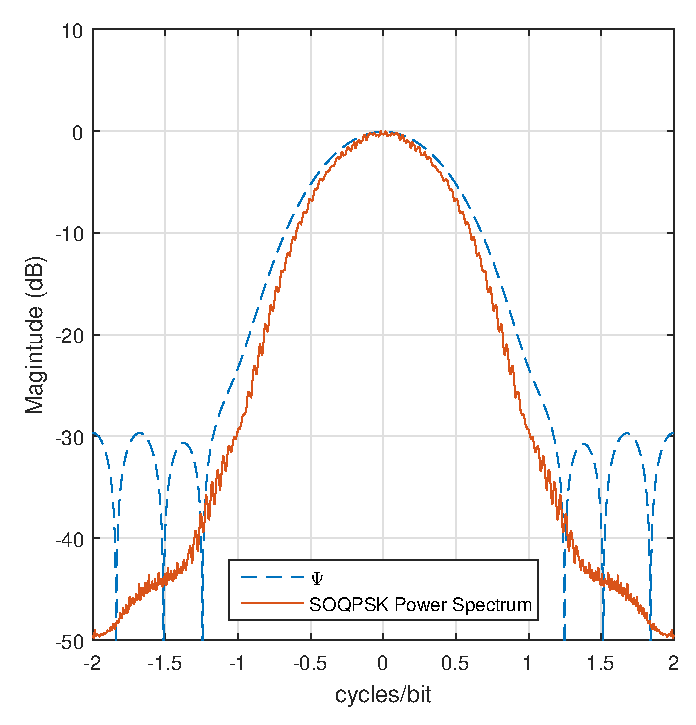
\includegraphics[width=5in]{figures/eq_equations/FDE2_spectrum_PSI.eps}
	\label{fig:SOQPSK_spectrum}
\end{figure}

\chapter{Equalizer GPU Implementation}
Each equalizer presents an intresting challenge from a GPU implementation perspective.
This is why in Chapter \ref{chap:eq_eq} the equalizer equations where massaged and conditioned.
This chapter will explain how the equalizers were computed and applied in batch processing.

Chapter \ref{chap:gpu_convolution} showed the true power of batched processing in GPUs.
Each batch of data is totally independent of other batches.
For this reason and to simplify figures, assume every block diagram in this chapter is duplicated $3104$ times on the GPU.
If a block diagram shows how to compute one equalizer coefficients vector, assume that the block diagram is repeated $3104$ times to compute $3104$ equalizer coefficent vectors.

Convolution is used many times in this chapter.
Frequency domain convolution has many little steps that make a block diagram look busy.
Figures \ref{fig:Conv2} and \ref{fig:Conv3} show how frequency domain convolution will be represented as one block from in this chapter.
\begin{figure}
	\caption{Convolution of vectors $\mathbf{c}$ and $\mathbf{r}$ block diagram simplified to one block marked Conv.}
	\centering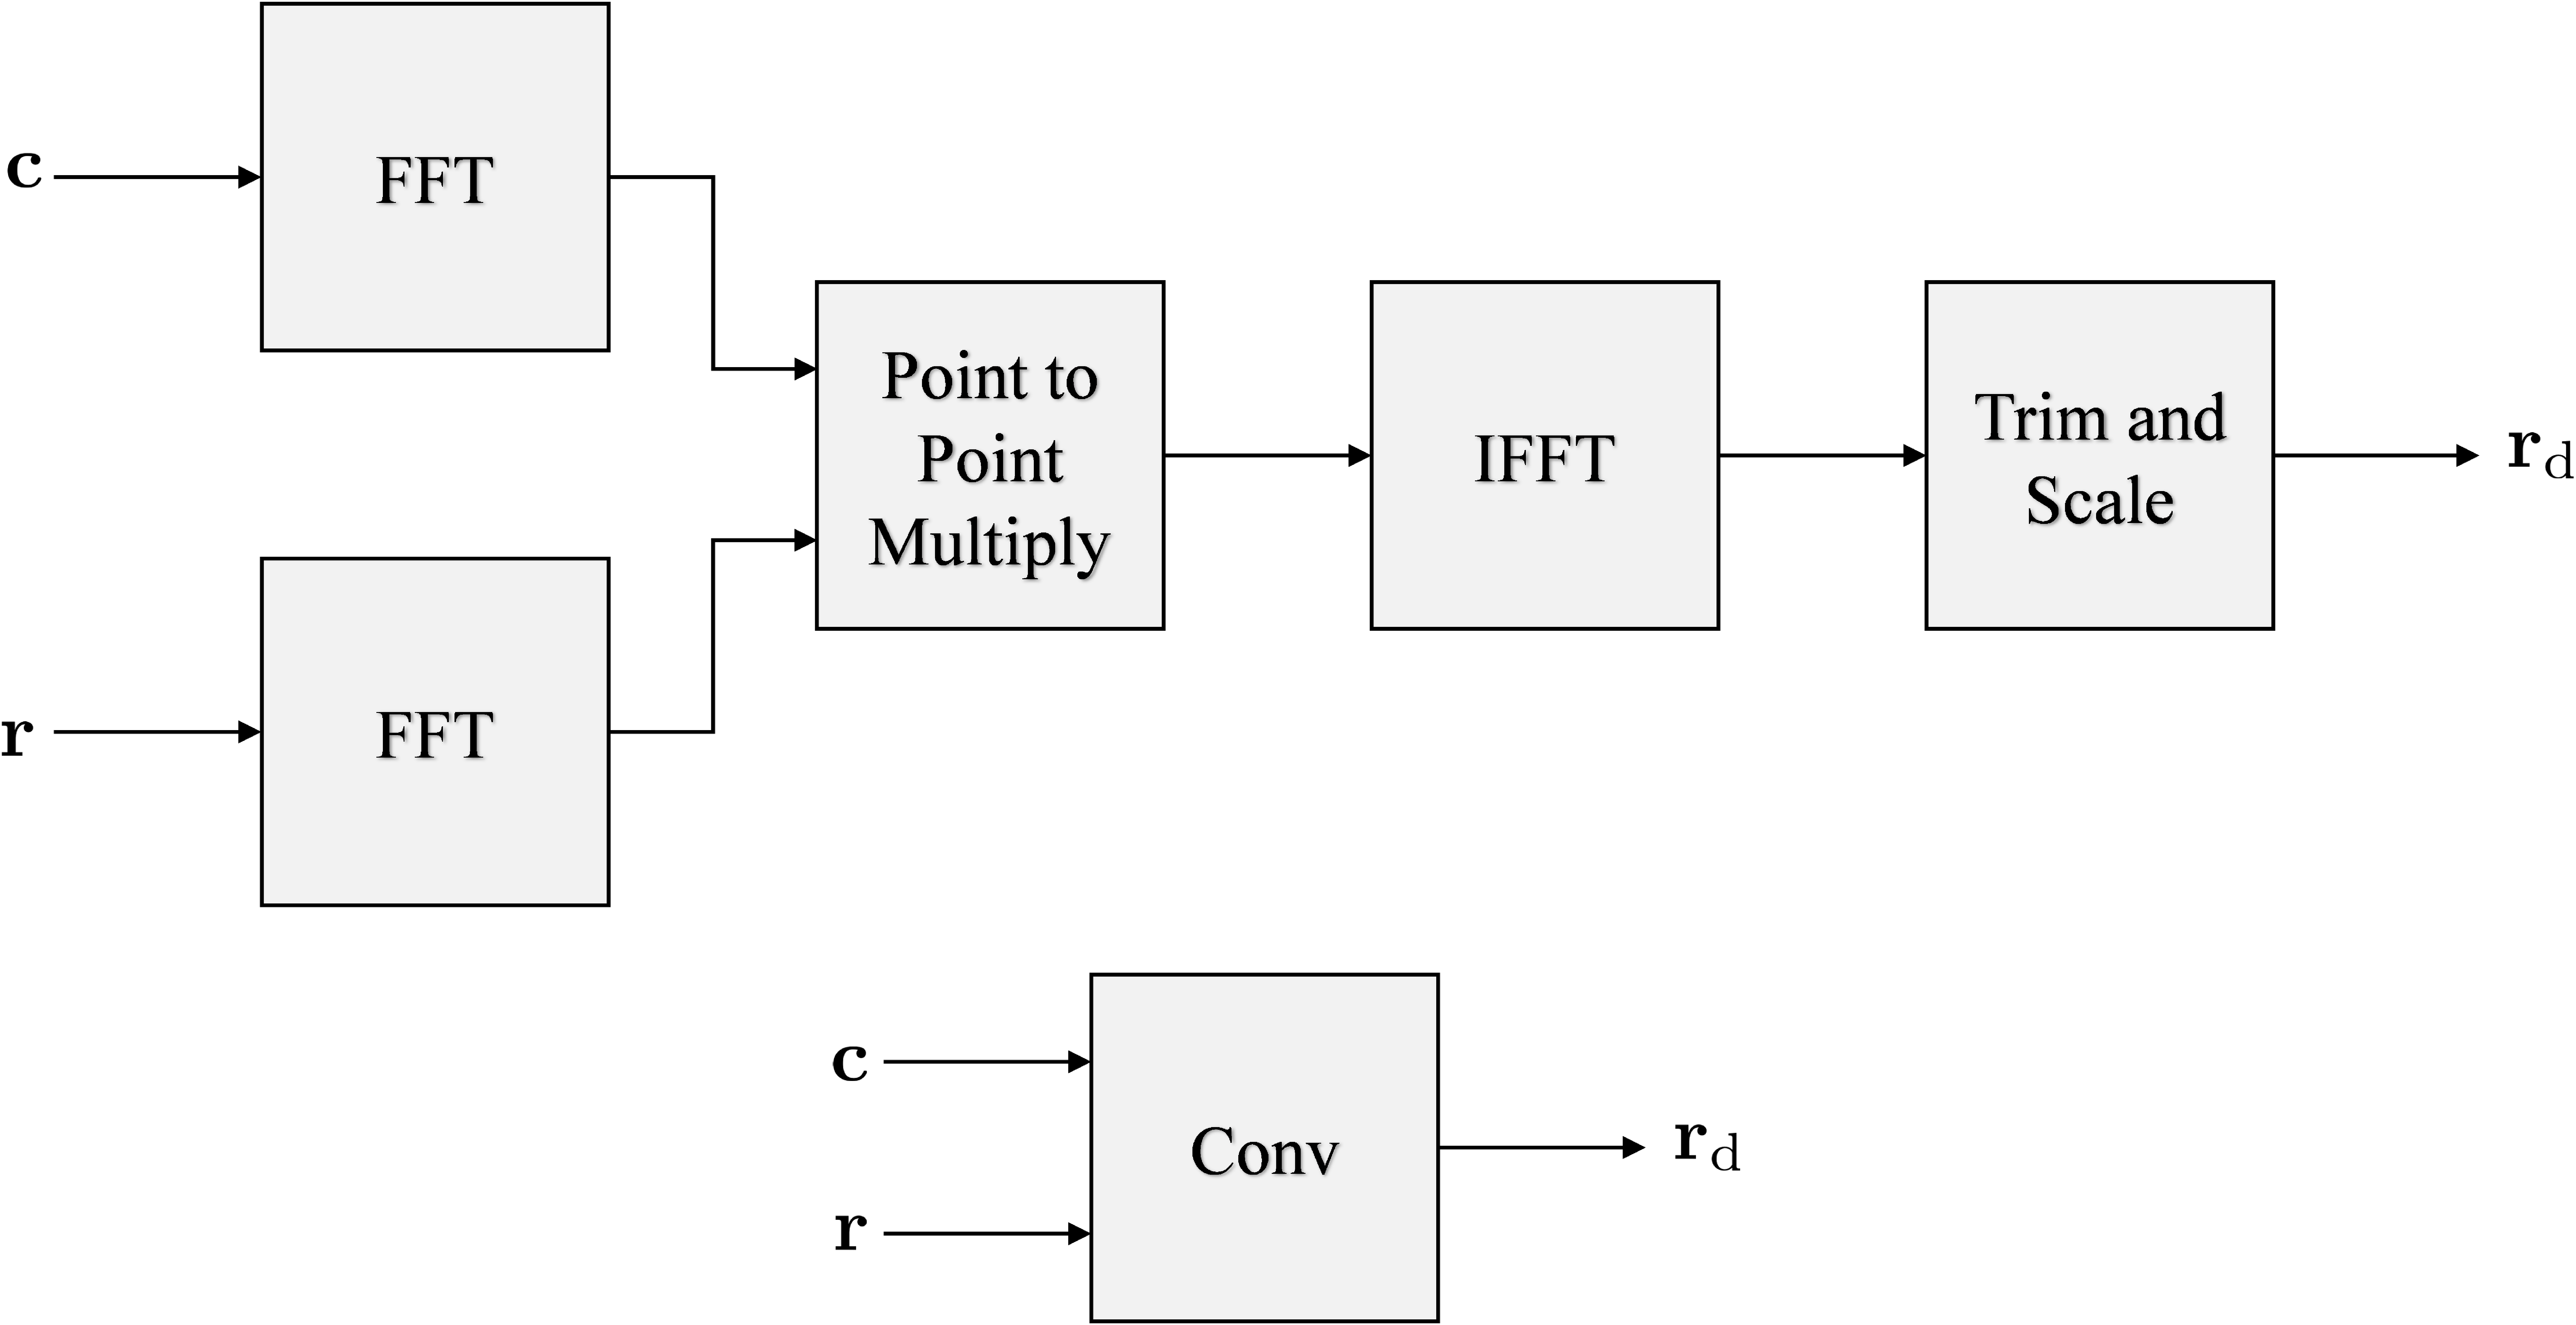
\includegraphics[width=9.27in/100*55]{figures/gpu_convolution/Conv2.pdf}
	\label{fig:Conv2}
\end{figure}
\begin{figure}
	\caption{Convolution of vectors $\mathbf{c}$, $\mathbf{r}$ and $\mathbf{H}_{\text{NO}}$ block diagram simplified to one block marked Conv.}
	\centering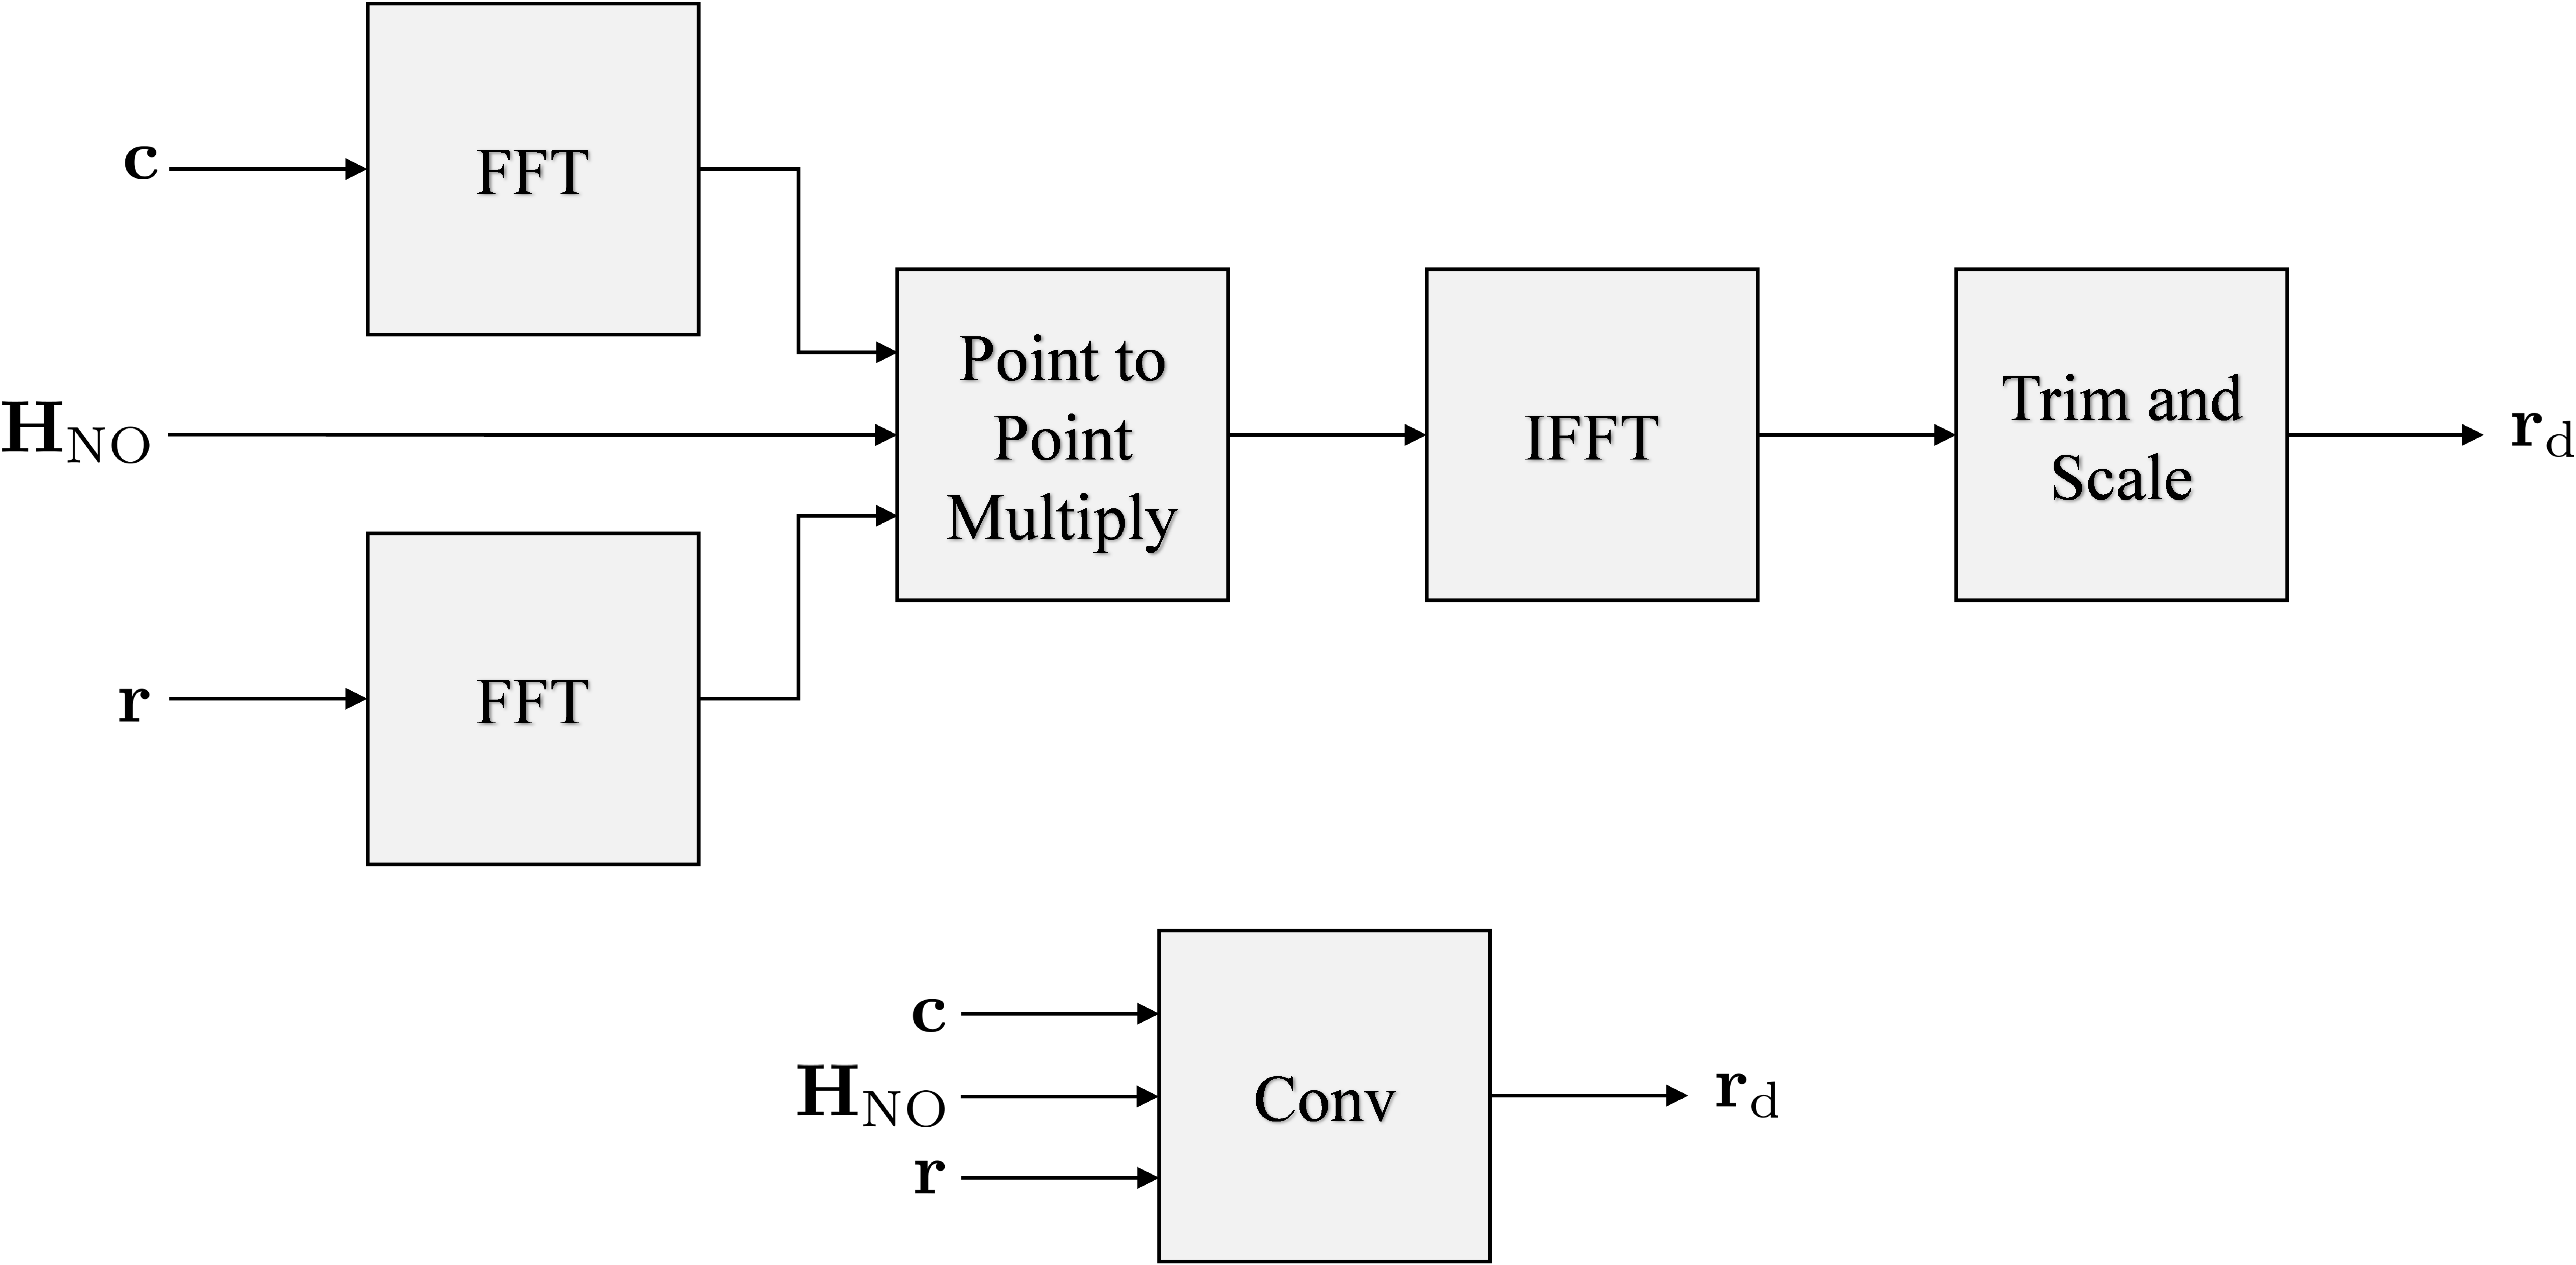
\includegraphics[width=9.27in/100*55]{figures/gpu_convolution/Conv3.pdf}
	\label{fig:Conv3}
\end{figure}


\section{Zero-Forcing and MMSE GPU Implementation}
The ZF and MMSE equalizer coefficient computations have exactly the same form as shown in Equations \ref{eq:c_ZF_solve} and \ref{eq:c_MMSE_solve}
\begin{equation}
\mathbf{R}_{\hat{h}} \mathbf{c}_\text{ZF} = \hat{\mathbf{h}}_{n_0}\\
\label{eq:ZF_gpuimp}
\end{equation}
\begin{equation}
\mathbf{R}_{\hat{h}w} \mathbf{c}_\text{MMSE} = \hat{\mathbf{h}}_{n_0}.
\label{eq:MMSE_gpuimp}
\end{equation}
The only difference is $\mathbf{R}_{\hat{h}}$ in ZF and $\mathbf{R}_{\hat{h}w}$ in MMSE.
Computing the ZF and MMSE equalizer coefficients is extremely computationally heavy.

It is possible to obtain the ZF and MMSE equalizer coefficients by computing the inverse of 
\begin{equation}
 \mathbf{c}_\text{ZF} = \mathbf{R}_{\hat{h}}^-1\hat{\mathbf{h}}_{n_0}
\label{eq:ZF_gpuimp}
\end{equation}
\begin{equation}
 \mathbf{c}_\text{MMSE} = \mathbf{R}_{\hat{h}w}^-1 \hat{\mathbf{h}}_{n_0}.
\label{eq:MMSE_gpuimp}
\end{equation}

Before solving Equation \ref{eq:ZF_gpuimp}, $\mathbf{R}_{\hat{h}}$ and $\hat{\mathbf{h}}_{n_0}$ need to be built and calculated given $\hat{\mathbf{h}}$.
The matrix $\mathbf{R}_{\hat{h}}$ requires the sample auto-correlation of the estimated channel $\mathbf{r}_{\hat{h}}$ and the time reversed channel and shifted channel $\hat{\mathbf{h}}_{n_0}$.

The vector $\hat{\mathbf{h}}_{n_0}$ is just the time reversed and conjugated estimated channel $\hat{\mathbf{h}}$. Building $\hat{\mathbf{h}}_{n_0}$ is trivial in the GPU and very little optimizing needs to be performed.
Computing the sample auto-correlation $\mathbf{r}_{\hat{h}}$ is done by implementing Equation \ref{eq:sample_autocorrelation} directly in one GPU kernel.
The computation of $\mathbf{r}_{\hat{h}}$ is very fast because the length of the channel estimate $L_{\text{ch}}$ is very short.

Section \ref{sec:zero-forcing} showed that $\mathbf{R}_{\hat{h}}$ is sparse because $r_{\hat{h}}(k)$ only has support on $-L_{\text{ch}} \leq k \leq L_{\text{ch}}$. 
To reduce computation time, the sparseness of $\mathbf{R}_{\hat{h}}$ will be leveraged. 
With out leveraging the sparse properties of $\mathbf{R}_{\hat{h}}$, even the mighty Tesla K40c cannot produce $\mathbf{c}_\text{ZF}$ in less than $500$ms.

The sparseness of $\mathbf{R}_{\hat{h}}$ is leveraged using a sparse solver function called ``cusolverSpCcsrqrsvBatched''.
cusolverSpCcsrqrsvBatched is a batched complex solver that leverages the sparse properties of $\mathbf{R}_{\hat{h}}$ by utilizing Compressed Row Storage (CRS) \cite{wiki:Sparse_matrix}.
The Compressed Row Storage reduces a large $186\times186$ matrix $\mathbf{R}_{\hat{h}}$ to a $12544$ element CSR matrix $\mathbf{R}_{\hat{h}\text{CRS}}$.
Before cusolverSpCcsrqrsvBatched can be called, the CSR matrix $\mathbf{R}_{\hat{h}\text{CRS}}$ has to be built using $\mathbf{r}_{\hat{h}}$.
An example of how to use the CUDA cusolverSp library can be found \cite{CUDA_toolkit_doc}.

Figure \ref{fig:blockZF} shows how the Zero-Forcing equalizer coefficients are implemented in the GPU.
\begin{figure}
	\caption{Block Diagram showing how the Zero-Forcing equalizer coefficients are implemented in the GPU.}
	\centering\includegraphics[width=7.5in/100*55]{figures/eq_GPUimplementation/blockZF.pdf}
	\label{fig:blockZF}
\end{figure}
The MMSE equalizer coefficients are computed nearly identically to ZF accept when calculating $\mathbf{R}_{\hat{h}w\text{CRS}}$, $\hat{\sigma}^2_w$ is added to the main diagonal elements.
\begin{figure}
	\caption{Block Diagram showing how the Minimum Mean Squared Error equalizer coefficients are implemented in the GPU.}
	\centering\includegraphics[width=7.98in/100*55]{figures/eq_GPUimplementation/blockMMSE.pdf}
	\label{fig:blockMMSE}
\end{figure}

Using cusolverSpCcsrqrsvBatched wasn't the only implementation researched.
Table \ref{tab:ZFMMSEtimingComparison} lists the algorithms researched and their respective execution times.
A custom GPU Levinson Recursion algorithm was built to leverage the Toeplitz structure of $\mathbf{R}_{\hat{h}}$ and $\mathbf{R}_{\hat{h}w}$ \cite[Chap. 5]{hayes:1996}. 
The Levinson Recursion algorithm initially showed promise when operating on real floats but when converted to complex data Levinson wasn't feasable.

Rather than solving for $\mathbf{c}_\text{ZF}$ or $\mathbf{c}_\text{MMSE}$, computing the full inverse of $\mathbf{R}_{\hat{h}}$ was researched using the cuBLAS LU Decomposition.
While using staying real time using cuBLAS was feasable, cusolverSp out performed cuBLAS by almost $2\times$.
\begin{table}
\caption{Defining start and stop lines for timing comparison in Listing \ref{code:convFun}.}
\begin{center}
\begin{tabular}{lll}
	\toprule
	Algorithm 			& Data type	& Execution Time (ms)	\\ \midrule
	Levinson Recursion 	& floats 	& 500 					\\
	Levinson Recursion 	& Complex 	& 2500 					\\
	LU Decomposition 	& Complex 	& 600				 	\\
	cuSolver			& Complex	& 355.96				\\
	\bottomrule
\end{tabular}
\end{center}
\label{tab:ZFMMSEtimingComparison}
\end{table}
%Jeff explains how CUDA solvers handle this equation.
%
%The ZF equalizer was studied in the PAQ Phase 1 Final Report in ~equation 324
%\begin{equation}
%\mathbf{c}_\text{ZF} = (\mathbf{H}^\dagger \mathbf{H})^{-1} \mathbf{H}^\dagger \mathbf{u}_{n_0}
%\label{eq:c_ZF_pinv}
%\end{equation}
%where $\mathbf{c}_\text{ZF}$ is a $L_{eq} \times 1$ vector of equalizer coefficients computed to invert the channel estimate $\hat{\mathbf{h}}$
%and $\mathbf{u}_{n_0}$ is the desired channel impulse response centered on $n0 = N_1+L_1+1$
%\begin{equation}
%\mathbf{u}_{n_0} = \begin{bmatrix} 0 \\ \vdots \\ 0 \\ 1 \\ 0 \\ \vdots \\ 0 \end{bmatrix}
%	\begin{matrix*}[l] \left. \vphantom{\begin{matrix} 0 \\ \vdots \\ 0 \end{matrix}} \right\}
%		\text{$n_0-1$ zeros}
%		\\ \\
%		\left. \vphantom{\begin{matrix} 0 \\ \vdots \\ 0 \end{matrix}} \right\}
%		\text{$N_1+N_2+L_1+L_2-n_0+1$ zeros}
%		\end{matrix*}.
%		\label{eq:un0_ZF}
%\end{equation}
%The $L_{eq}+N_1+N_2 \times L_{eq}$ convolution matrix $\mathbf{H}$ is built using the channel estimate $\hat{\mathbf{h}}$
%\begin{equation}
%\mathbf{H} = 
%		\begin{bmatrix}
%		h(-N_1)		&  			& 		 	&  			\\
%		h(-N_1+1) 	& h(-N_1)	& 		 	&  			\\
%		\vdots	 	& \vdots	& \ddots 	&  			\\
%		h(N_2)		& h(N_2-1) 	&  			& h(-N_1)  	\\
%		 			& h(N_2) 	&  			& h(-N_1+1) \\
%		 			&  	   		&  			& \vdots	\\
%		 			&  	   		&  			& h(N_2)	\\
%	\end{bmatrix}.
%\end{equation}
%The computation of the coefficients in Equation \eqref{eq:c_ZF_pinv} can be simplified in a couple of ways: First the matrix multiplication of $\mathbf{H}^\dagger$ and $\mathbf{H}$ is the autocorrelation matrix of the channel
%\begin{equation}
%\mathbf{R}_{\hat{h}} = 
%\mathbf{H}^\dagger \mathbf{H} = 
%		\begin{bmatrix}
%		r_{h}(0)		& r^\ast_{h}(1)	& \cdots 	& r^\ast_{h}(L_{eq}-1)  	\\
%		r_{h}(1) 		& r_{h}(0)		& \cdots 	& r^\ast_{h}(L_{eq}-2)  	\\
%		\vdots	 			& \vdots				& \ddots 	&  							\\
%		r_{h}(L_{eq}-1)	& r_{h}(L_{eq}-2)	& \cdots	& r_{h}(0)  			
%	\end{bmatrix}
%	\label{eq:R_h}
%\end{equation}
%where
%\begin{equation}
%r_{h}(k) = \sum_{n=-N_1}^{N_2} h(n) h^\ast(n-k).
%\end{equation}
%Second the matrix vector multiplication of $\mathbf{H}^\dagger$ and $\mathbf{u}_{n_0}$ is simply the $n_0$th row of $\mathbf{H}^\dagger$ or the conjugated $n_0$th column of $\mathbf{H}$.
%A new vector $\hat{\mathbf{h}}_{n_0}$ is defined by
%\begin{equation}
%\hat{\mathbf{h}}_{n_0} = \mathbf{H}^\dagger \mathbf{u}_{n_0} = 
%\begin{bmatrix} h(L_1) \\ \vdots \\ h(0) \\ \vdots \\ h(-L_2)  \end{bmatrix}.
%\label{eq:h_no}
%\end{equation}
%To simplify, Equations \eqref{eq:R_h} and \eqref{eq:h_no} are substituted into Equation \eqref{eq:c_ZF_pinv} resulting in 
%\begin{equation}
%\mathbf{c}_\text{ZF} = \mathbf{R}^{-1}_{h} \hat{\mathbf{h}}_{n_0}.
%\label{eq:c_ZF_R_h}
%\end{equation}
%
%Computing the inverse of $\mathbf{R}_{\hat{h}}$ is computationally heavy because an inverse is an $N^3$ operation.
%To avoid an inverse, $\mathbf{R}_{\hat{h}}$ is moved to the left side and $\mathbf{c}_\text{ZF}$ is found by solving a system of linear equations. 
%Note that $r_{h}(k)$ only has support on $-L_{ch} \leq k \leq L_{ch}$ making $\mathbf{R}_{\hat{h}}$ sparse or $\%63$ zeros.
%The sparseness of $\mathbf{R}_{\hat{h}}$ is leveraged to reduce computation drastically.
%The Zero-Forcing Equalizer coefficients are computed by solving
%\begin{equation}
%\mathbf{R}_{\hat{h}} \mathbf{c}_\text{ZF} = \hat{\mathbf{h}}_{n_0}.
%\label{eq:c_ZF_solve}
%\end{equation}


\section{Constant Modulus Algorithm GPU Implementation}
The Constant Modulus Algorithm (CMA) is quite a bit more complicated than all other equalizers.
CMA presented real challenges when implementing into a GPU.
The direct approach didn't allow for multiple iterations.
The more iterations CMA performed, the better CMA becomes becouse CMA is a steepest decent.

Each iteration of CMA uses the signal equalized by the most recent $\mathbf{c}_{\text{CMA}b}$
\begin{equation}
\mathbf{y} = \mathbf{r}*\mathbf{c}_{\text{CMA}b}.
\end{equation}
The element of the gradient $\nabla J(k)$ is calculate by convolving the $12672$ sample $\mathbf{z}$ and with the $12672$ sample $\rho$. 
Note that all other frequency domain convolutions in this Thesis are $\text{Nfft} = 2^{14}$, but the convolution length $12672+12672-1>2^{14}$. The FFTs in the computation of $\nabla J(k)$ are $\text{Nfft} = 2^{15}$ point FFTs.
The element  of the gradient vector $\nabla J(k)$ is calculated by
\begin{equation}
\nabla J(k) = \frac{1}{L_{pkt}} b(k), \quad -L_1 \leq k \leq L_2
\end{equation}
where
\begin{align}
b(n) &= \sum^{L_{pkt}-1}_{m=0} z(m) \rho(n-m) \nonumber \\
	 &= \sum^{L_{pkt}-1}_{m=0} z(m) r^\ast(m-n)
\end{align}
using convolution.
Once $\nabla J$ is calculated, the steepest decent algorithm is applied
\begin{equation}
\mathbf{c}_\text{CMA($b+1$)} = \mathbf{c}_\text{CMA($b$)}-\mu \nabla J.
\end{equation}
The goal of CMA is to perform as many iterations as possible.
Once done iterating, apply the last $\mathbf{c}_\text{CMA($b+1$)}$ to the received signal $\mathbf{r}$.

In Section \ref{sec:CMA}, the direct application of CMA was massaged into convolution.
Figure \ref{fig:blockCMA} shows a block diagram of how the CMA algorithm runs on the GPU.
\begin{figure}
	\caption{Diagram showing the relationships between $z(n)$, $\rho(n)$ and $b(n)$.}
	\centering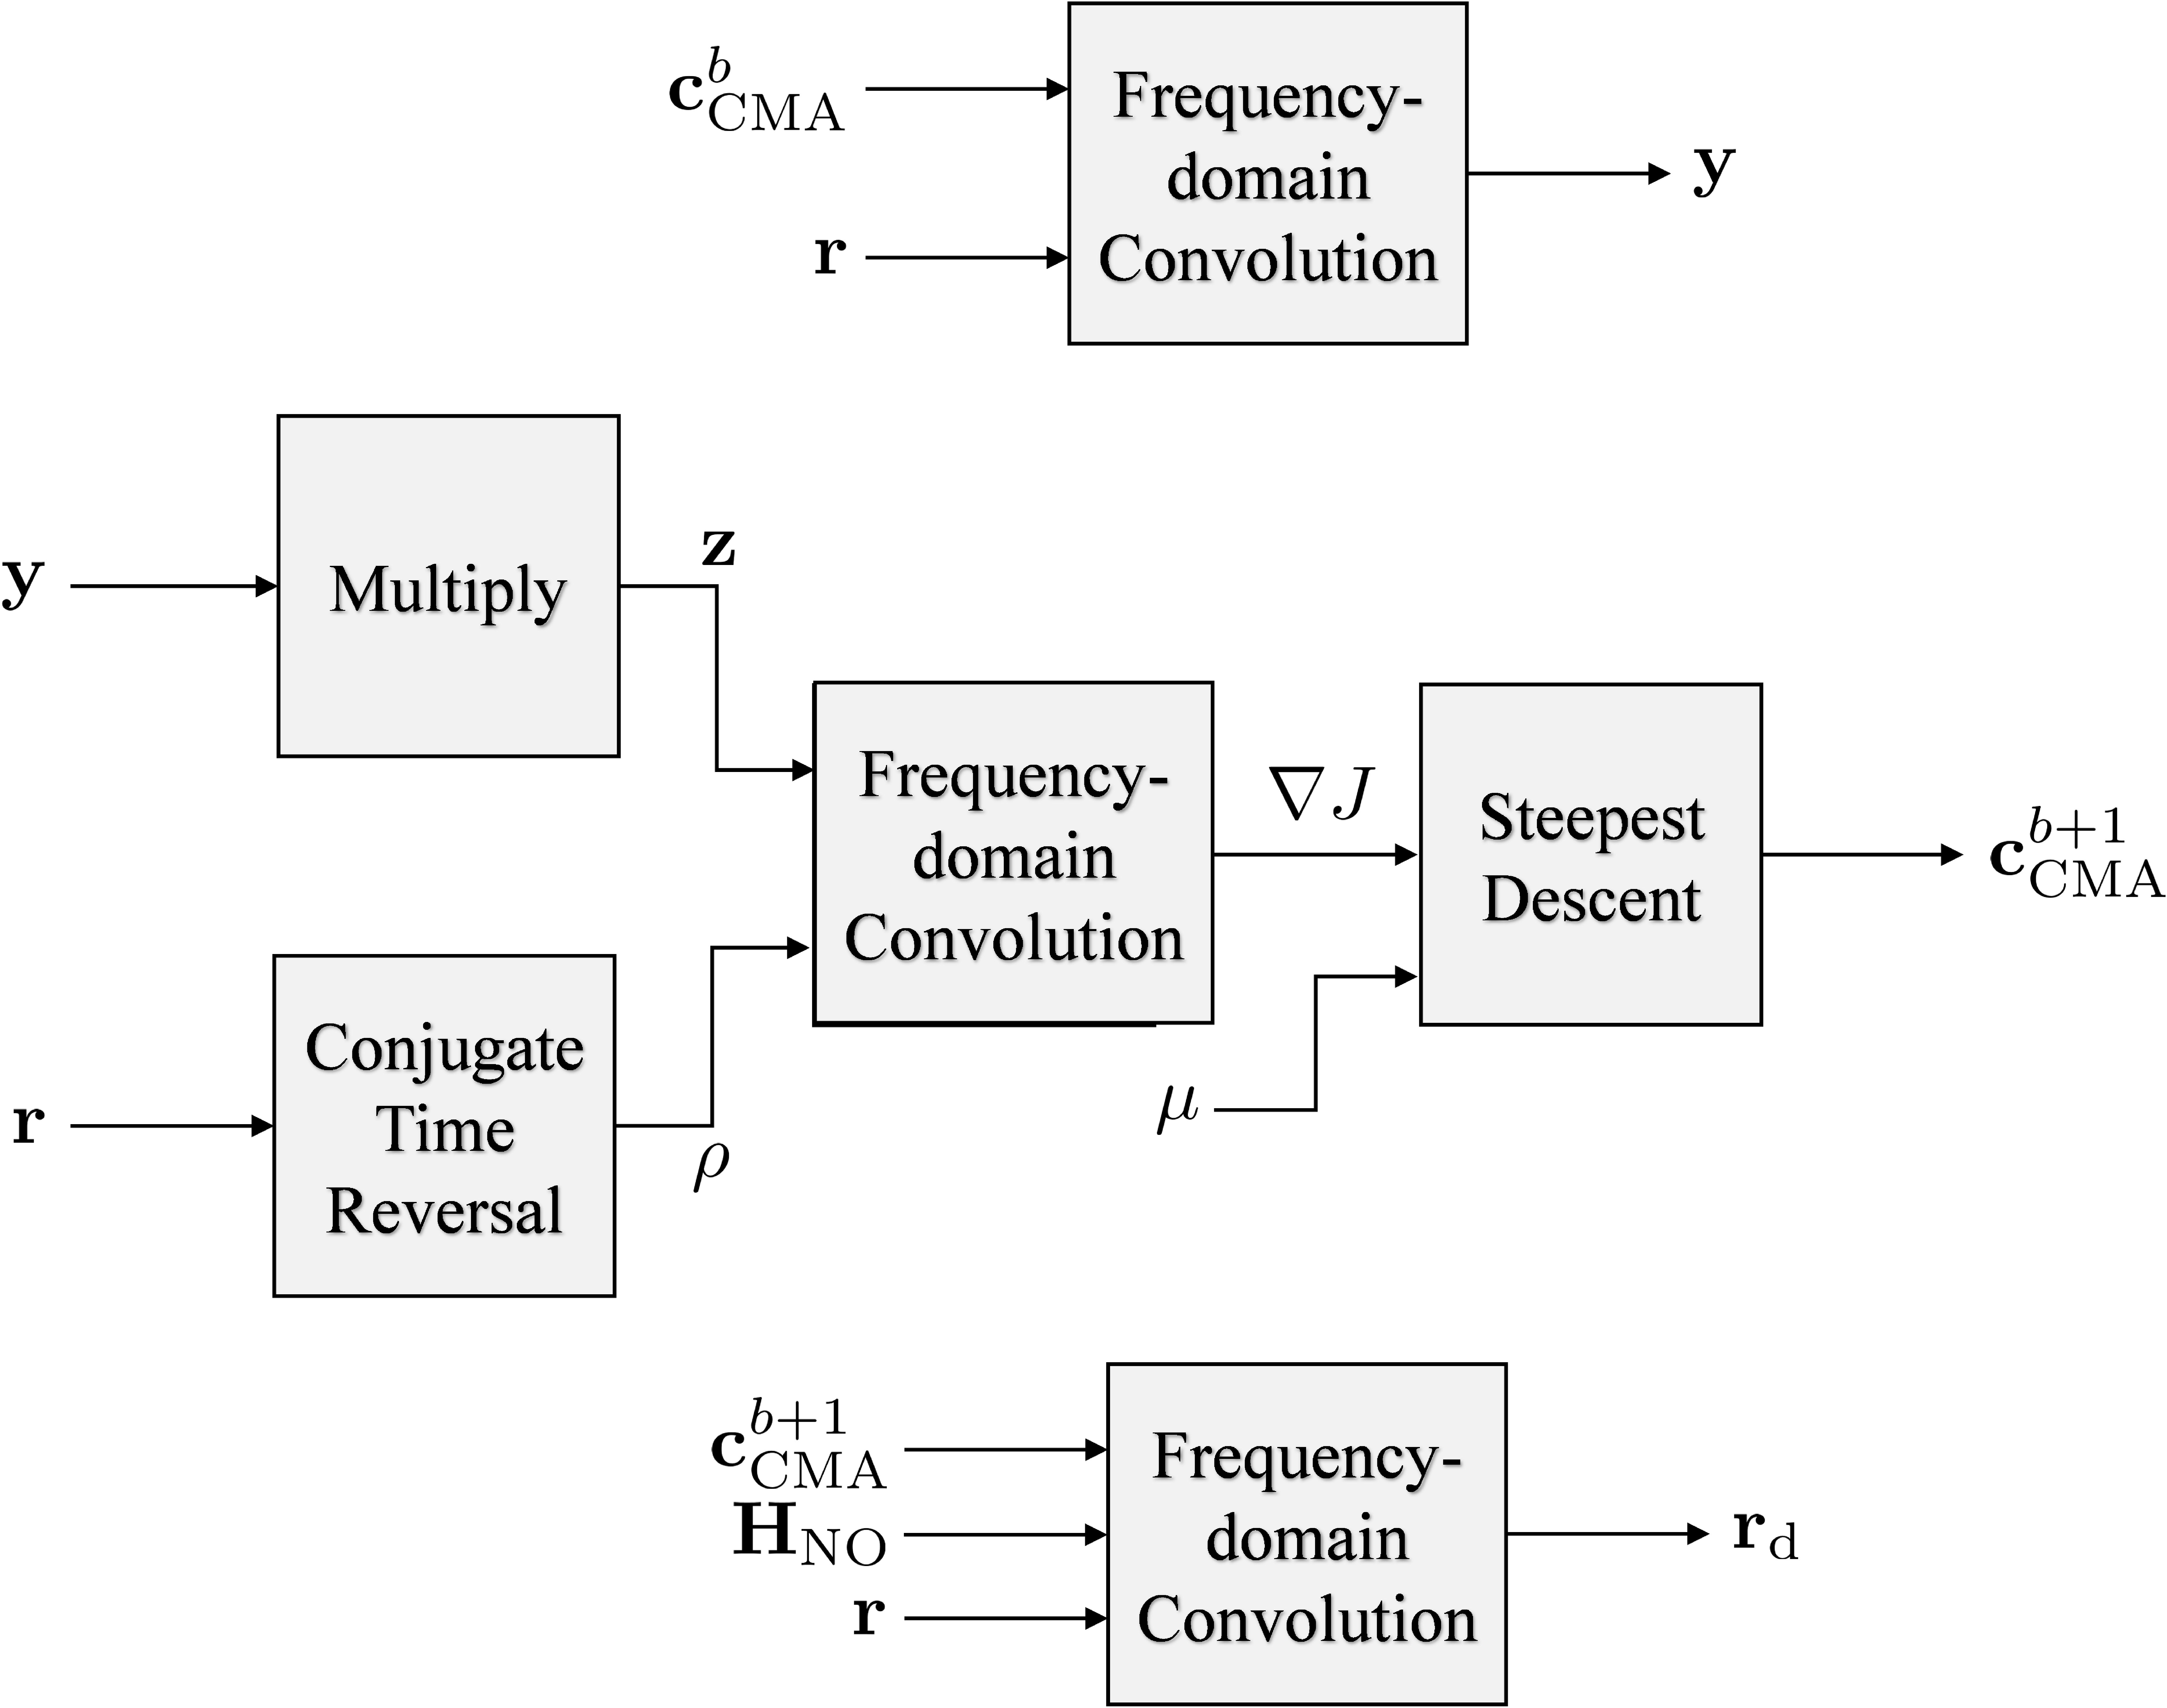
\includegraphics[width=8.34in/100*55]{figures/eq_GPUimplementation/blockCMA.pdf}
	\label{fig:blockCMA}
\end{figure}

The most computationally heavy part of CMA is computing $\nabla J(k)$.
Computing $\nabla J(k)$ directly is almost $5\times$ slower than using convolution.
The direct computation is done by performing a long $12672$ sample summation from Equation \ref{eq:delJ_direct_way}
\begin{equation}
\nabla J(k) = \frac{1}{L_{pkt}} \sum^{L_{pkt}-1}_{m=0}  z(m) r^\ast(m-k), \quad -L_1 \leq k \leq L_2.
\end{equation}
Long summations are slow in GPUs.
Table \ref{tab:CMAtimingComparison} lists the comparison on computing $\nabla J(k)$ verse using convolution.
\begin{table}
\caption{The gradient vector $\nabla J(k)$ can be computed using convolution or computed directly.}
\begin{center}
\begin{tabular}{lll}
	\toprule
	CMA	Iteration Algorithm			& Execution Time (ms)	\\ \midrule
	$\nabla J$ directly 			& 421.317				\\
	$\nabla J$ using convolution & 88.7743				\\
	\bottomrule
\end{tabular}
\end{center}
\label{tab:CMAtimingComparison}
\end{table}



\section{Frequency Domain Equalizer One and Two GPU Implementation}
The Frequency Domain Equalizers are by far the fastest and easiest to implement into GPUs.
The block diagram looks just like convolution accept that point to point multiply isn't a simple two or three point complex multiply.

Equation \ref{eq:FDE1} and is implemented directly in the GPU.
To save execution time, the FFT of the detection filter $\mathbf{H}_{\text{NO}}$ multiplied at the same time FDE1 is calculated 
\begin{equation}
R_\text{d1}(e^{j\omega_k}) = \frac{R(e^{j\omega_k}) \hat{H}^\ast(e^{j\omega_k}) H_{\text{NO}}(e^{j\omega_k})}  {|\hat{H}(e^{j\omega_k})|^2  +  \frac{1}{\hat{\sigma}^2_w}} \quad
\text{where} \;
\omega_k = \frac{2\pi}{L} \;
\text{for} \;
k=0,1,\cdots,L-1
\label{eq:FDE1_applied}
\end{equation}
\begin{equation}
R_\text{d2}(e^{j\omega_k}) = \frac{R(e^{j\omega_k}) \hat{H}^\ast(e^{j\omega_k}) H_{\text{NO}}(e^{j\omega_k})}  {|\hat{H}(e^{j\omega_k})|^2  +  \frac{\Psi(e^{j\omega_k})}{\hat{\sigma}^2_w}} \quad
\text{where} \;
\omega_k = \frac{2\pi}{L} \;
\text{for} \;
k=0,1,\cdots,L-1
\label{eq:FDE2_applied}
\end{equation}
where $R(e^{j\omega_k})$ and $R_\text{d}(e^{j\omega_k})$ is the FFT $\mathbf{r}$ and $\mathbf{r}_\text{d}$ 
at $\omega_k$.
\begin{table}
\caption{Defining start and stop lines for timing comparison in Listing \ref{code:convFun}.}
\begin{center}
\begin{tabular}{lll}
	\toprule
	Algorithm						& Execution Time (ms)	\\ \midrule
	Frequency Domain Equalizer One 	& 57.156				\\
	Frequency Domain Equalizer Two	& 58.841				\\
	\bottomrule
\end{tabular}
\end{center}
\label{tab:CMAtimingComparison}
\end{table}
Figures \ref{fig:blockFDE1} and \ref{fig:blockFDE2} show block diagrams of how FDE1 and FDE2 are implemented in the GPUs.
\begin{figure}
	\caption{Diagram showing Frequency Domain Equalizer One is implemented in the frequency domain in GPUs.}
	\centering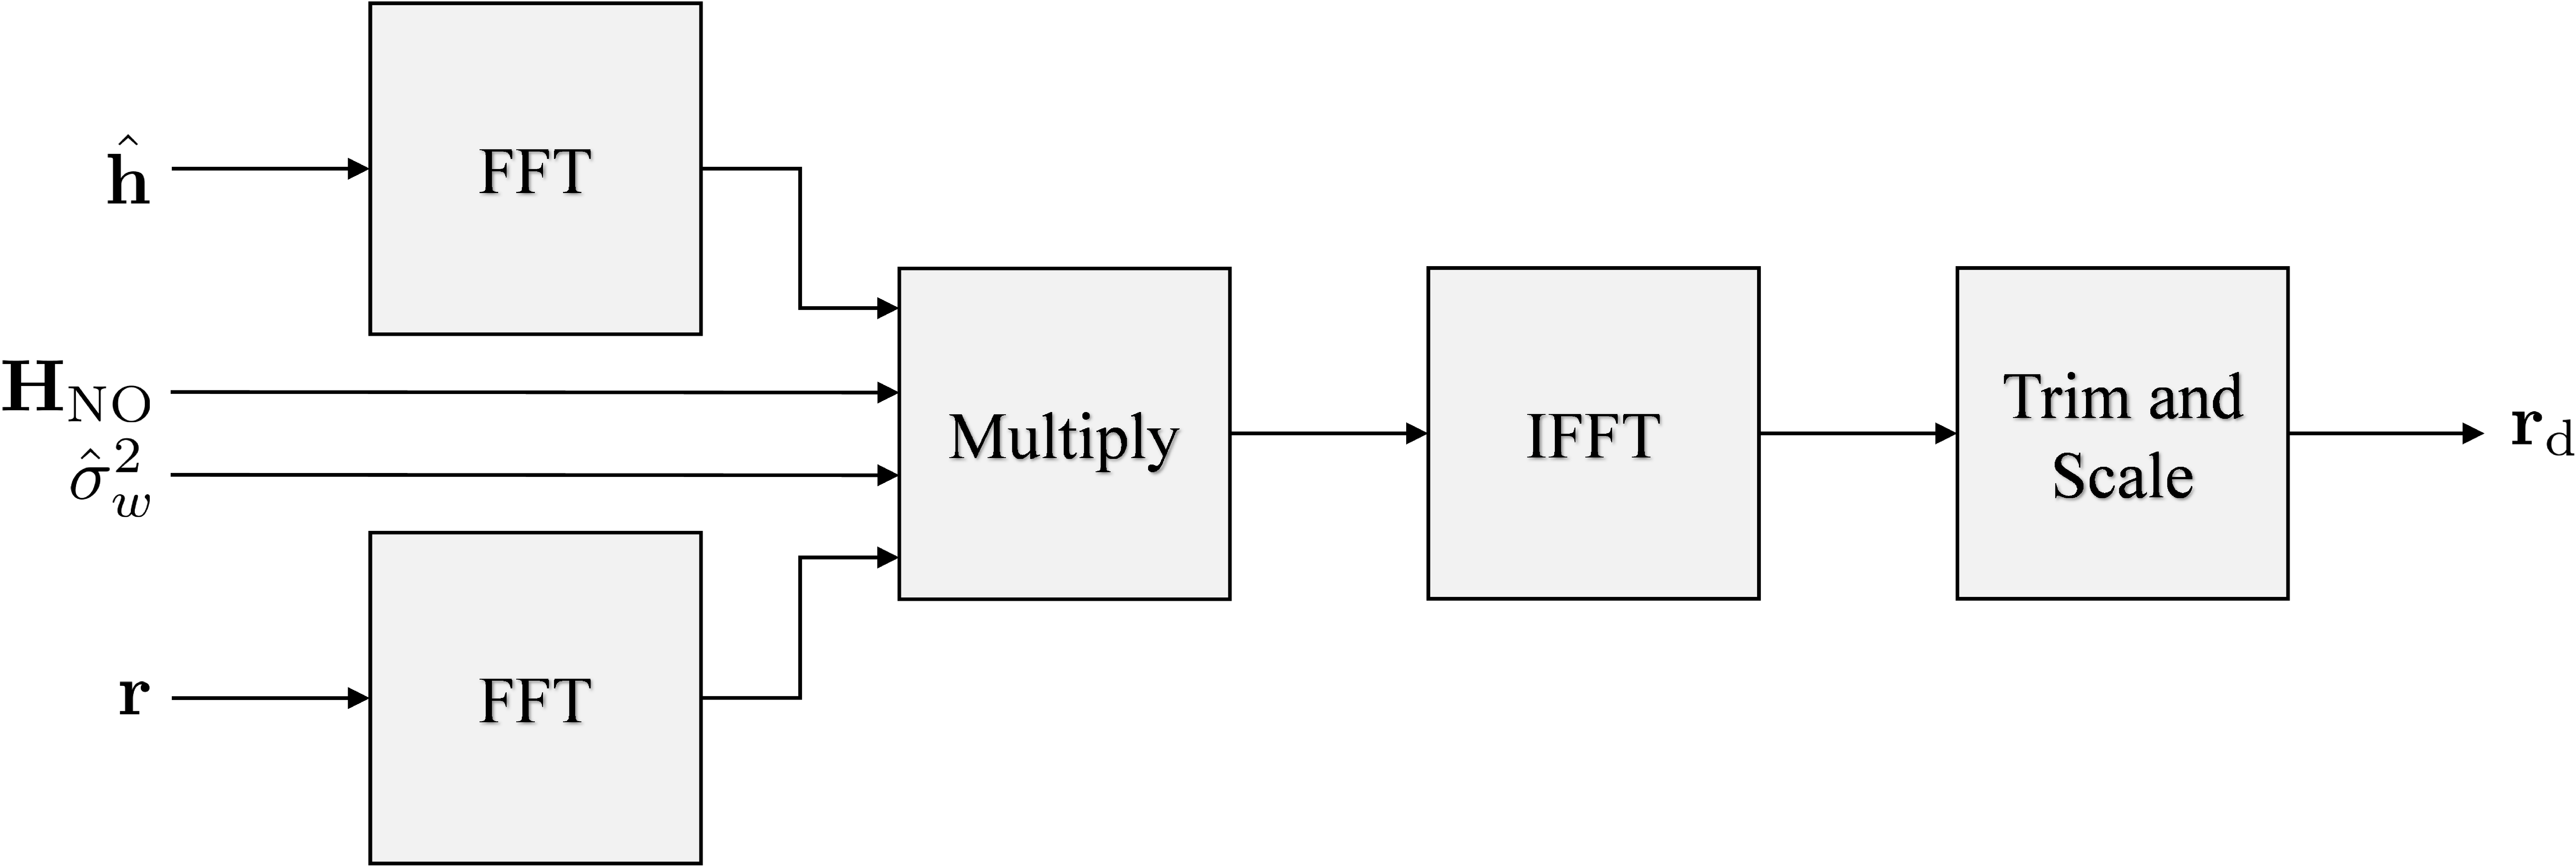
\includegraphics[width=9.73in/100*55]{figures/eq_GPUimplementation/blockFDE1.pdf}
	\label{fig:blockFDE1}
\end{figure}
\begin{figure}
	\caption{Diagram showing Frequency Domain Equalizer Two is implemented in the frequency domain in GPUs.}
	\centering\includegraphics[width=10.03in/100*55]{figures/eq_GPUimplementation/blockFDE2.pdf}
	\label{fig:blockFDE2}
\end{figure}






\chapter{Summary and Conclusions}
\label{chap:final_summary}
\section{GPU Implementation}
Based on measured execution times of GPU kernels, multiple data-aided equalization filters where implemented for the purpose of equalizing an aeronautical telemetry channel.
Using GPU libraries and batch processing rather than custom designed GPU kernels produced massive speed ups.
Also, reformulating algorithms into frequency-domain convolution produced impressive speed ups.

For implementation in one Tesla K40c and two Tesla K20c GPUs the execution times for all equalizers met the real-time constraint.
It was shown that the frequency-domain equalizers are the easiest to implement and have the fastest execution time.
The CMA equalizer was shown to be the hardest to implement and has the slowest execution time.
The execution time did not provide the CMA the opportunity to iterate many times.
The ZF and MMSE equalizers were shown to be computationally challenging to implement but had an acceptable execution time.

Because data-aided equalizers are implemented for a real-time telemetry receiver system,
the execution time results must be considered along with the bit error rate performance.
%Despite the performance of the CMA equalizer in AWGN, the execution time per iteration does not allow the equalizer to converge in multipath.
As of this writing the FDE1 equalizer is recommended, marking the best tradeoff between performance and computational complexity.

\section{Contributions}
Through the years of working on the PAQ project I:
\begin{enumerate}
\item Implemented algorithms using batch GPU libraries to reduce execution time on average by 5.
\item Reduced GPU convolution time by using batch GPU librarys and cascading filters in the frequency domain.
\item Implemented linear solver libraries to make ZF and MMSE equalizers feasible and real-time.
\item Reformulated the CMA to leverage the speed of GPU convolution.
\item Implemented new ADC to drive success of the PAQ project.
\item Implemented resampling polyphase filters in GPUs.
\item Participated heavily in flight tests at Edwards AFB.
\item Presented a paper frequency offset compensation for equalized SOQPSK at International \newline Telemetering. Conference (ITC) \cite{ravert2016}.
\end{enumerate}

\section{Further Work}
The Levinson-Durbin algorithm GPU implementation only leveraged the toeplitz structure of the channel estimate auto-correlation matrix.
A hybrid sparse Levinson-Durbin algorithm could leverage the sparseness of the channel estimate auto-correlation matrix and the vector $\hat{\mathbf{h}}_{n_0}$.




%%%%%%%%%%%%% begin Bibliography %%%%%%%%%%%%%%%%%
\phantomsection %Forces a new section prior to setting the bibliography reference point
\bibliographystyle{IEEEtran}
\addcontentsline{toc}{chapter}{Bibliography}
\bibliography{refs}

% Bibliographies are best created and maintained using BibTeX
% To use Bibtex, create a bibliography file, e.g., refs.bib
% The sample file sources.bib shows examples of different
% bibliographic entries.
% The bibliography is created by executing:
%  1.  latex, 2. bibtex, 3. latex, 4. latex
%%%%%%%%%%%%%%%% end Bibliography %%%%%%%%%%%%%%%%%

%Included because WinEdit is RETARDED and it needs it for Gather Purposes:
%input "refs.bib"


% Include appendix sections here:
% each appendix should be a file with a .tex extension and the text
% of the file should begin with \appendix{Appendix Title}, followed
% by the contents of the appendix
%\appendix{Sample Appendix}

\section{Width Based on Page Size Figure Example} \label{sec:appendxia_figure_example}
Here's an example of a figure whose width depends on the width
of the page. You can see if as Figure \ref{fig:appendix_some_pic}.

\begin{figure}[htbp]
  \centering
  \includegraphics[width=0.45\textwidth]{figures/appendixa/some_pic}
  \caption[Example Width Based on Page Size Figure]{
    This is an example of a figure whose width will be 45\% of the
    width of the page. If you'd like to see a figure with a fixed
    width then you can see it as Figure \ref{fig:intro_stuff} in
    Section \ref{sec:intro_figure_example}. Just FYI, I made this
    figure with PowerPoint and then copied it and pasted it into
    wmf2eps and choose the "Paste EMF" option. It will generate
    a larger file, but it will look a TON better than the
    "Paste WMF" option and the "Paste DIB" option will paste the
    rasterized image that won't scale well at all.}
  \label{fig:appendix_some_pic}
\end{figure}

%End the document
\end{document}
